% Vorlesung 13.12.18 (11 Days until christmas)


% ab Hier auch richtige Phi und keine varPhis

\chapter{Zeitabhängige elektromagnetische Felder - Elektrodynamik}

bisher Zeitunabhängige Felder:
\begin{equation*}
\, \vabla \cdot \vec{D} = \rho \qquad \, \vabla \times \vec{E} = 0 \qquad \tx{Elektrostatik}
\end{equation*}
\begin{equation*}
\ \ \: \vabla \cdot \vec{B} = 0 \qquad \vabla \times \vec{H} = \vec{j} \qquad \tx{Magnetostatik}
\end{equation*}
Zeitabhängige Felder:
\begin{equation*}
\vec{B}(\vec{r}, t) \leftrightarrow \vec{E}(\vec{r}, t)
\end{equation*}

\section{Maxwell-Gleichungen}

\begin{align*}
\vabla \cdot \vec{D} &= \rho \qquad \, \vabla \times \vec{E} + \prt{\vec{B}}{t} = 0 \\
\vabla \cdot \vec{B} &= 0 \qquad \vabla \times \vec{H} - \prt{\vec{D}}{t} = \vec{j}
\end{align*}
$ \prt{\vec{B}}{t} \ $ ist die Induktion\\[3pt]
$ \prt{\vec{D}}{t} \ $ ist der Verschiebungsstrom\\

\subsection{Faraday'sches Induktionsgesetz}

\begin{equation*}
\vabla \times \vec{E} = - \prt{\vec{B}}{t}
\end{equation*}
\begin{center}
	%t1: %t2:
	\begin{tikzpicture}
	% \draw (0,0) ellipse (1cm and .7cm);
	\coordinate (r) at (-2.2,0);
	\draw[->] ($ ({cos(45) * -.9},{sin(45) * -.6}) + (r) $) arc[start angle=-135, end angle=225, x radius = .9cm, y radius = .6cm] node[anchor=north east] {$ \partial F $};
	\draw[->] ($ ({cos(45) * .9},{sin(45) * .6}) + (r) $) arc[start angle=-315, end angle=45, x radius = .9cm, y radius = .6cm];
	\node at (r) {$ F $};
	\node[left] at ($ (r) + (-1,0) $) {$ U_{\tx{ind}} $};
	\draw[fill=gray!30!white] (-.3,-.7) rectangle node[] {$ \substack{\tx{\Large{S}} \\[10pt] \tx{\Large{N}}} $} (.3,.7);
	\draw[->] (0,0) -- (.7,0) node[right] {$ \vec{v} $};
	
	\draw[looseness=2] (.15,.7) to[out=80,in=90] (1.2,0) to[out=-90,in=-80] (.15,-.7);
	\draw[looseness=2] (.09,.7) to[out=84,in=90] (1.8,0) to[out=-90,in=-84] (.09,-.7);
	\draw[looseness=2.5] (.03,.7) to[out=88,in=90] (2.6,0) to[out=-90,in=-88] (.03,-.7);
	
	\draw[looseness=2] (-.15,.7) to[out=100,in=90] (-1.2,0) to[out=-90,in=-100] (-.15,-.7);
	\draw[looseness=2] (-.09,.7) to[out=96,in=90] (-1.8,0) to[out=-90,in=-96] (-.09,-.7);
	\draw[looseness=2.5] (-.03,.7) to[out=92,in=90] (-2.6,0) to[out=-90,in=-92] (-.03,-.7);
	\end{tikzpicture}
\end{center}
\begin{align*}
\int_F \dd \vec{f} \cdot (\vec{\nabla} \times \vec{E}) &= - \int \dd \vec{f} \cdot \prt{\vec{B}}{t} = \ub{\int_{\partial F} \dd \vec{r} \cdot \vec{E}}_{U_{\tx{ind}}} = - \prd{}{t} \ub{\int_F \dd \vec{f} \cdot \vec{B}}_{\Phi_m (t)}
\end{align*}
$ \Phi_m(t) $ ist der Fluss des $ \vec{B} $-Feldes durch F
\begin{equation*}
U_{\tx{ind}} = - \prd{}{t} \int_F \dd \vec{f} \cdot \vec{B}
\end{equation*}
\emph{Bemerkung:}
\begin{enumerate}[i)]
	\item Vorzeichen-Strom
	\begin{center}
			%t3:
			\begin{tikzpicture}[scale=1.25]
				\coordinate (a) at (0,0);
				\draw[->] ($ ({cos(45) * -.9},{sin(45) * -.6}) + (a) $) arc[start angle=-135, end angle=225, x radius = .9cm, y radius = .6cm] node[anchor=north east] {$ \partial F $};
				\draw[->] ($ ({cos(45) * .9},{sin(45) * -.6}) + (a) $) arc[start angle=-45, end angle=315, x radius = .9cm, y radius = .6cm] node[anchor=north west] {$ \vec{j} $};
				\draw[thick,->] ($ (a) + (.3,-.3) $) -- ++(0,1.2);
				\draw ($ (a) + (.4,0) $) -- ++(1,.5) node[right] {$ \vec{B}(t_1) = \vec{B}_1 $};
				\draw[thick,->] ($ (a) + (-.3,.3) $) -- node[left=10pt] {$ \dd \vec{f} $} ++(0,.6);
				
				\coordinate (b) at (6,0);
				\draw[->] ($ ({cos(45) * -.9},{sin(45) * -.6}) + (b) $) arc[start angle=-135, end angle=225, x radius = .9cm, y radius = .6cm] node[anchor=north east] {$ \partial F $};
				\draw[->] ($ ({cos(45) * .9},{sin(45) * -.6}) + (b) $) arc[start angle=-45, end angle=315, x radius = .9cm, y radius = .6cm] node[anchor=north west] {$ \vec{j} $};
				\draw[thick,->] ($ (b) + (.3,-.3) $) -- ++(0,.6);
				\draw ($ (b) + (.4,0) $) -- ++(1,.5) node[right] {$ \vec{B}(t_2) = \vec{B}_2 $};
				\draw[thick,->] ($ (b) + (-.3,.3) $) -- node[left=10pt] {$ \dd \vec{f} $} ++(0,.6);
			\end{tikzpicture}
	\end{center}
	\begin{equation*}
	t_2 > t_1 \qquad \vec{B}(t_1) > \vec{B}(t_2)
	\end{equation*}
	\begin{equation*}
	\Phi_m(t_1) = \int_F \dd \vec{f} \vec{B}_1 > \Phi_m(t_2) = \int_F \dd \vec{f} \vec{B}_2
	\end{equation*}
	\begin{equation*}
	\prd{}{t} \Phi_m(t) \le 0
	\end{equation*}
	\begin{equation*}
	\rightarrow \quad U_{\tx{ind}} = \int_{\partial F} \dd \vec{r} \cdot \vec{E} = - \prd{}{t} \Phi_m > 0
	\end{equation*}
	Mit $ \vec{j} = \sigma \vec{E} $, wobei $ \sigma $ die Leitfähigkeit des Leiters ist erhalten wir:
	\begin{equation*}
	\rightarrow \quad \int_{\partial F} \dd \vec{r} \cdot \vec{j} > 0 \qquad \rightarrow \quad \vec{j} \parallel \partial F
	\end{equation*}
	\begin{minipage}{.5\linewidth}
		$ \Rightarrow $ \textbf{Lenz'sche Regel:}\\
		Der induzierte Strom und das damit verbundene Magnetfeld sind so gerichtet, dass sie der Ursache ihrer Entstehung entgegenwirken.
	\end{minipage}%
	\begin{minipage}{.5\linewidth}
		\flushright
		%t4:
		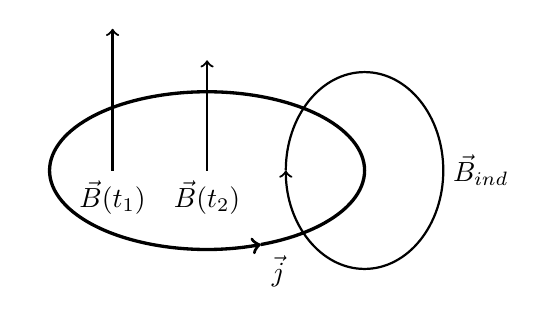
\begin{tikzpicture}
			\draw[->,very thick] ({cos(70) * 2cm}, {sin(70) * -1cm}) arc[start angle=-70, end angle=290,x radius = 2cm, y radius = 1cm] node[anchor=north west] {$ \vec{j} $};
			\draw[->, thick] (1,0) arc[start angle=180,end angle=-180,x radius=1cm, y radius=1.25cm];
			\node[right] at (3,0) {$ \vec{B}_{\tx{ind}} $};
			\foreach \x\n\l in {-1.2/1/1.8,0/2/1.4}
			\draw[thick,->] (\x,0) node[below] {$ \vec{B}(t_{\n}) $} -- ++(0,\l);
		\end{tikzpicture}
	\end{minipage}%
	\\
	Hier fällt das äußere $ \vec{B} $-Feld ab, wodurch ein Strom entsteht, der wiederum ein $ \vec{B} $-Feld $ \vec{B}_{\tx{ind}} $ induziert welches gegen den Abfall wirkt, also das äußere $ \vec{B} $-Feld verstärkt.
	\item $ \Phi_m $ hängt nicht von der speziellen Form der Fläche $ F $ ab, sondern nur vom Rand $ \partial F $.\\
	\begin{center}
		%t5:
		\begin{tikzpicture}
			\coordinate (c1) at (0,0);
			\draw[fill=blue!30!white,->] ($ (c1) + ({sin(45) * 1cm},{cos(45) * -.5cm}) $) arc[start angle=-45, end angle=315, x radius=1cm, y radius=.5cm] node[anchor=north west] {$ \partial F $};
			\draw[->] ($ (c1) + (.25,.25) $)  -- node[right] {$ \dd\vec{f}_1 $} ++(0,1);
			\draw ($ (c1) + (-.5,-.25) $) to[out=-130,in=-20] ++(-1,-.2) node[left] {$ F_1 $};
			
			\coordinate (c2) at (4,0);
			\draw[fill=red!30!white,looseness=2] ($ (c2) + (-1,0) $) to[out=-90,in=-90] ($ (c2) + (1,0) $);
			\draw[fill=red!13!white,->] ($ (c2) + ({sin(45) * 1cm},{cos(45) * -.5cm}) $) arc[start angle=-45, end angle=315, x radius=1cm, y radius=.5cm] node[xshift=.7cm] {$ \partial F $};
			\draw[->] ($ (c2) + (.25,-.3) $)  -- node[right,yshift=10pt] {$ \dd\vec{f}_2 $} ++(0,1.55);
			\draw ($ (c2) + (.6,-.8) $) to[out=-50,in=200] ++(1,-.2) node[right] {$ F_2 $};
			\node at ($ (c2) + (3.5,0) $) {$ \Phi_{m_1} = \Phi_{m_2} $};
			
			\coordinate (c3) at (2,-3);
			\draw[fill=red!30!white,looseness=2] ($ (c3) + (-1,0) $) to[out=-90,in=-90] ($ (c3) + (1,0) $);
			\draw[fill=blue!30!white] ($ (c3) + ({sin(45) * 1cm},{cos(45) * -.5cm}) $) arc[start angle=-45, end angle=315, x radius=1cm, y radius=.5cm];
			\draw[->] ($ (c3) + (-.25,.25) $)  -- node[left=5pt] {$ \dd\vec{f}_1 $} ++(0,1);
			\draw[->] ($ (c3) + (.25,-.75) $) -- node[right=5pt] {$ - \dd \vec{f_2} $} ++(0,-1);
		\end{tikzpicture}
	\end{center}
	
	\noindent
	Aus der Skizze und mit Satz von Gauß. (Der Fluss durch eine geschlossene Fläche ist gleich 0):
	\begin{equation*}
	\Phi = \int_F \dd \vec{f} \cdot \vec{B} = 0
	\end{equation*}
	\begin{equation*}
	\Phi_{\tx{m}_1} = \Phi_{\tx{m}_2}
	\end{equation*}
	\begin{equation*}
	0 = \int_F \dd \vec{f} \cdot \vec{B} = \ub{\int_{F_1} \dd \vec{f}_1 \cdot \vec{B}}_{\Phi_{\tx{m}_1}} - \ub{\int_{F_2} \dd \vec{f}_2 \cdot \vec{B}}_{\Phi_{\tx{m}_2}}
	\end{equation*}
	\item Eine Flussänderung kann auf verschiedene Weise zustandekommen:\\
	\begin{minipage}{.5\linewidth}
		\begin{itemize}
			\item Veränderung des Magnetfeldes $ \vec{B}(t) $
			\item Bewegung der Leiterschleife im äußeren Feld
		\end{itemize}
		\begin{equation*}
		\vabla \times \vec{E} = - \prt{\vec{B}}{t}
		\end{equation*}
		\vspace{20pt}
	\end{minipage}%
	\begin{minipage}{.5\linewidth}
		\flushright
		%t6:
		\begin{tikzpicture}[scale=1]
			\coordinate (r) at (-2.2,0);
			\draw[thick,->] ($ ({cos(45) * -.9},{sin(45) * -.6}) + (r) $) arc[start angle=-135, end angle=225, x radius = .9cm, y radius = .6cm];
			\draw[fill=gray!30!white] (-.3,-.7) rectangle node[] {$ \substack{\tx{\Large{S}} \\[8pt] \tx{\Large{N}}} $} (.3,.7);
			\draw[thick,->] (0,0) -- (1.1,0) node[right] {$ \vec{v} $};
			\draw[thick,->] ($ (r) + (-1,0) $) -- ++(-1.1,0);
			
			\draw[looseness=2] (.15,.7) to[out=80,in=90] (1.2,0) to[out=-90,in=-80] (.15,-.7);
			\draw[looseness=2] (.09,.7) to[out=84,in=90] (1.8,0) to[out=-90,in=-84] (.09,-.7);
			\draw[looseness=2.5] (.03,.7) to[out=88,in=90] (2.6,0) to[out=-90,in=-88] (.03,-.7);
			
			\draw[looseness=2] (-.15,.7) to[out=100,in=90] (-1.2,0) to[out=-90,in=-100] (-.15,-.7);
			\draw[looseness=2] (-.09,.7) to[out=96,in=90] (-1.8,0) to[out=-90,in=-96] (-.09,-.7);
			\draw[looseness=2.5] (-.03,.7) to[out=92,in=90] (-2.6,0) to[out=-90,in=-92] (-.03,-.7);
		\end{tikzpicture}
	\end{minipage}%
	\\
	Ein zeitlich verändertes $ \vec{B} $-Feld erzeugt ein elektrisches Wirbelfeld analog zu:
	\begin{equation*}
	\vabla \times \vec{B} = \mu_0 \vec{j}
	\end{equation*}
	\begin{center}
		%t7:
		\begin{tikzpicture}
		\draw[very thick, ->] (0,-1) -- (0,1) node[left] {$ \vec{j} $};
		\draw[->] ({.5 * sin(45)},-{.25 * cos(45)}) arc[start angle=-45,end angle=315, x radius=.5, y radius=.25];
		\draw[->] ({1 * sin(45)},-{.5 * cos(45)}) arc[start angle=-45, end angle=315, x radius=1, y radius=.5];
		\node at (.7,-.7) {$ \vec{B} $};
		
		\coordinate (a) at (3,0);
		\draw[very thick, ->] ($ (a) + (-.175,-1) $) -- ++(0,2);
		\draw[very thick, ->] ($ (a) + (.175,-1) $) -- ++(0,2);
		\draw[->] ($ (a) + ({.5 * sin(45)},-{.25 * cos(45)}) $) arc[start angle=-45,end angle=315, x radius=.5, y radius=.25];
		\draw[->] ($ (a) + ({1 * sin(45)},-{.5 * cos(45)}) $) arc[start angle=-45, end angle=315, x radius=1, y radius=.5];
		\node at ($ (a) + (1,-1) $) {$ \prt{\vec{B}}{t} $};
		\end{tikzpicture}
	\end{center}
\end{enumerate}

\subsection{Maxwellscher Verschiebungsstrom}

Magnetostatik:
\begin{equation*}
\vabla \times \vec{H} = \vec{j} \qquad \tx{Amp\`ere}
\end{equation*}
Dies kann in der Elektrodynamik nicht gelten, dies zeigen wir indem wir auf beiden Seiten die Divergenz bilden.
\begin{equation*}
\ub{\vabla \cdot (\vabla \times \vec{H})}_{=0} = \vabla \cdot \vec{j} \quad \Rightarrow \quad \vabla \cdot \vec{j} = 0 \quad \tx{bei stationären Strömen}
\end{equation*}
im Allgemeinen haben wir zeitlich abhängige Ströme:
\begin{equation*}
\vabla \cdot \vec{j}(\vec{r},t) \overset{\tx{i.A.}}{\neq} 0
\end{equation*}
Kontinuitätsgleichung:
\begin{equation*}
\prt{\rho}{t} + \vabla \cdot \vec{j} = 0
\end{equation*}
Ergänzung:
\begin{equation*}
\vabla \times \vec{H} = \vec{j} + \vec{j}_0
\end{equation*}
\begin{equation*}
\Rightarrow \quad \ub{\vabla \cdot (\vabla \times \vec{H})}_{= 0} = \ub{\vabla \cdot \vec{j}}_{= - \prt{\rho}{t}} + \vabla \cdot \vec{j}_0
\end{equation*}
\begin{equation*}
\Rightarrow \quad \vabla \cdot \vec{j}_0 = \prt{\rho}{t} = \prt{}{t} \vabla \cdot \vec{D} = \vabla \cdot \left(\prt{\vec{D}}{t}\right)
\end{equation*}
\begin{equation*}
\rightarrow \quad \vec{j}_0 = \prt{\vec{D}}{t}
\end{equation*}
Damit erhalten wir für die die Stromdichte:
\begin{equation*}
\vabla \times \vec{H} - \prt{\vec{D}}{t} = \vec{j}
\end{equation*}
\emph{Beispiel:} \textbf{Plattenkondensator}\\
\begin{minipage}{.6\linewidth}
	\begin{equation*}
	\vec{D} = \casess{\sigma \vec{e}_x}{\tx{innen}}{0}{\tx{außen}}
	\end{equation*}
	$ \sigma = \frac{q}{F} $
	\begin{equation*}
	\prt{\vec{D}}{t} = \frac{\vec{e}_x}{F} \equalto{\prd{q}{t}}{I} = \frac{I}{F} \vec{e}_x
	\end{equation*}
	\begin{equation*}
	\vabla \times \vec{H} - \prt{\vec{D}}{t} = \vec{j}
	\end{equation*}
	innen: $ \vec{j} = 0 $
	\begin{equation*}
	\vabla \times \vec{H} = \prt{\vec{D}}{t} =  \frac{I}{F} \vec{e}_x
	\end{equation*}
\end{minipage}%
\begin{minipage}{.4\linewidth}
	\flushright
	%t8:
	\begin{tikzpicture}[scale=1]
		\draw[very thick] (-1.5,-2) -- (-1.5,2) node[above] {$ q $};
		\draw[very thick] (1.5,-2) -- (1.5,2) node[above] {$ - q $};
		
		\foreach \y in {-1.8,-.6,.6,1.8}
		\draw[->] (-1.3,\y) -- (1.3,\y);
		
		\foreach \y in {-1.8,-.6,.6,1.8}
		\draw[fill = white!20!red] (-1.8,\y) circle (.2cm) node[] {$ \color{white} + \color{white} $};
		
		\foreach \y in {-1.8,-.6,.6,1.8}
		\draw[fill = white!20!blue] (1.8,\y) circle (.2cm) node[] {$ \color{white} - \color{white} $};
		
		\node at (0,1.2) {$ \vec{D} $};
		\node at (0,-1.2) {$ \vec{H} $};
		
		\draw[->] (0,-3) -- ++(1.5,0) node[right] {$ x $};
		\draw (0,-3.1) -- (0,-2.9);
		
		\draw[very thick] (-1.5,-2) -- (-1.5,-2.5);
		\draw[very thick] (1.5,-2) -- (1.5,-2.5);
		\draw[->] (-1.5,-2.5) -| (-3,-4) -- (0,-4) node[below] {\Large{$ I $}};
		\draw (1.5,-2.5) -| (3,-4) -- (0,-4);
		\draw[thick,->] ($ (-2.5,-2.5) + ({sin(45) * .3},{cos(45) * -.8}) $) arc[start angle=-45, end angle=315, x radius=.3, y radius=.8];
		\draw[thick,->] ($ (2.5,-2.5) + ({sin(45) * .3},{cos(45) * -.8}) $) arc[start angle=-45, end angle=315, x radius=.3, y radius=.8];
	\end{tikzpicture}
\end{minipage}%

\subsection{Lösung der Differentialgleichungen} %check this

\begin{align*}
\vabla \cdot \vec{D} &= \rho \qquad \, \vabla \times \vec{E} + \prt{\vec{B}}{t} = 0 \\
\vabla \cdot \vec{B} &= 0 \qquad \vabla \times \vec{H} - \prt{\vec{D}}{t} = \vec{j}
\end{align*}
Zwei homogene und zwei inhomogene Differentialgleichungen. Zur Lösung benötigt man also zusätzliche Materialgleichungen:
\begin{equation*}
\vec{B} = \mu_0 (\vec{H} + \vec{M}) \qquad \vec{D} = \epsilon_0\vec{E} + \vec{P}
\end{equation*}
bei linearen Medien:
\begin{equation*}
\vec{B} = \mu \vec{H} \qquad \vec{D} = \epsilon \vec{E}
\end{equation*}
Die Kraft ist:
\begin{equation*}
\vec{F} = q (\vec{E} + \vec{v} \times \vec{B})
\end{equation*}
\textbf{Intagrale Form der Maxwell-Gleichungen}
\begin{align*}
\oint_{\partial V} \dd \vec{f} \cdot \vec{B} &= 0  \qquad \qquad \qquad \qquad \: \oint_{\partial F} \dd \vec{r} \cdot \vec{E} + \prd{}{t} \int_F \dd \vec{f} \cdot \vec{B} = 0 \\
\oint_{\partial V} \dd \vec{f} \cdot \vec{D} &= \int_V \dd^3 r \rho(\vec{r}) = Q \quad \ \ \oint_{\partial F} \dd \vec{r} \cdot \vec{H} - \prd{}{t} \int_F \dd \vec{f} \cdot \vec{D} = \int_F \dd \vec{f} \cdot \vec{j} = I
\end{align*}
\textbf{Mikroskopische Maxwell-Gleichungen:}\\
formal:
\begin{equation*}
\vec{D} = \epsilon_0 \vec{E} \qquad \vec{H} = \frac{1}{\mu_0} \vec{B}
\end{equation*}
\begin{align*}
\vabla \cdot \vec{B} &= 0 \qquad \quad \vabla \times \vec{E} + \prt{\vec{B}}{t} = 0\\
\vabla \cdot \vec{E} &= \frac{1}{\epsilon_0} \rho \qquad \vabla \times \vec{B} - \epsilon_0 \mu_0 \prt{\vec{E}}{t} = \mu_0 \vec{j}
\end{align*}

\section{Potentiale der Elektrodynamik - Eichtransformation}

\begin{equation*}
\vabla \cdot \vec{B} = 0 \qquad \rmbox{\vec{B}(\vec{r},t) = \vabla \times \vec{A}(\vec{r},t)}
\end{equation*}
\begin{align*}
\vabla \times \vec{E} + \prt{\vec{B}}{t} = 0 \qquad 0 &= \vabla \times \vec{E} + \prt{}{t} \vabla \times \vec{A} \\
&= \vabla \times \left(\vec{E} + \prt{\vec{A}}{t}\right)
\end{align*}
\begin{equation*}
\Rightarrow \quad \vec{E} + \prt{\vec{A}}{t} = - \vabla \Phi
\end{equation*}
$ \Phi $ ist ein skalares Potential
\begin{equation*}
\Rightarrow \quad \rmbox{\vec{E}(\vec{r},t) = - \vabla \Phi(\vec{r},t) - \prt{\vec{A}(\vec{r},t)}{t}}
\end{equation*}
Damit haben wir die beiden homogenen Gleichungen gelöst. Wir können $ \vec{E} $- und $ \vec{B} $-Felder nun durch die Potentiale $ \Phi $ und $ \vec{A} $ ausdrücken.

\subsection{Bestimmungsgleichung für \texorpdfstring{$ \Phi , \vec{A} $}{phi A}}

\begin{equation*}
\vec{D} = \epsilon \vec{E} \qquad \vec{H} = \frac{1}{\mu} \vec{B}
\end{equation*}
\begin{align*}
\rightarrow \quad \vabla \cdot \vec{E} = \frac{1}{\epsilon} \rho
\end{align*}
\begin{equation*}
\frac{1}{\epsilon} \rho = \vabla \cdot \left(- \vabla \Phi - \prt{\vec{A}}{t}\right) = - \Delta \Phi - \prt{}{t} \vabla \cdot \vec{A}
\end{equation*}
\begin{equation*}
\rmbox{\Rightarrow \quad \Delta \Phi + \prt{}{t} \vabla \cdot \vec{A} = - \frac{1}{\epsilon} \rho}
\end{equation*}
\begin{align*}
& \vabla \times \vec{B} - \epsilon \mu \prt{\vec{E}}{t} = \mu \vec{j}
\end{align*}
\begin{equation*}
\mu \vec{j} = \ub{\vabla \times (\vabla \times \vec{A})}_{=\vabla \cdot (\vabla \cdot \vec{A}) - \Delta \vec{A}} - \epsilon \mu \prt{}{t} \left(- \vabla \Phi - \prt{\vec{A}}{t}\right)
\end{equation*}
\begin{equation*}
\rmbox{\Rightarrow \quad \Delta \vec{A} - \epsilon \mu \prt{^2 \vec{A}}{t^2} - \vabla \cdot \left(\vabla \cdot \vec{A} + \epsilon \mu \prt{\Phi}{t}\right) = - \mu \vec{j}}
\end{equation*}

\subsection{Eichtransformation}

$ \Phi, \vec{A} $ sind durch:
\begin{equation*}
\vec{B} = \vabla \times \vec{A} \qquad \vec{E} = - \vabla \Phi - \prt{\vec{A}}{t}
\end{equation*}
nicht eindeutig festgelegt.\\[5pt]
\textbf{Eichtransformation:}
\begin{align*}
\vec{A}'(\vec{r},t) &= \vec{A}(\vec{r},t) + \vabla \Lambda(\vec{r},t)\\
\Phi'(\vec{r},t) &= \Phi(\vec{r},t) - \prt{\Lambda(\vec{r},t)}{t}
\end{align*}
\begin{equation*}
\vabla \times \vec{A}' = \vabla \times \vec{A} + \ub{ \vabla \times (\vabla \Lambda)}_{=0} = \vabla \times \vec{A} = \vec{B} \quad \checkmark
\end{equation*}
\begin{equation*}
- \vabla \Phi' - \prt{\vec{A}'}{t} = - \vabla \Phi + \cancel{\vabla \prt{\Lambda}{t}} - \prt{\vec{A}}{t} - \cancel{\prt{}{t} \vabla \Lambda} = \vec{E} \quad \checkmark 
\end{equation*}
$ \rightarrow $ verschiedene Eichungen.
\begin{enumerate}[1)]
	\item \textbf{Coulomb-Eichung}
	\begin{equation*}
	\vabla \cdot \vec{A}(\vec{r},t) = 0
	\end{equation*}
	\begin{equation*}
	\rmbox{\rightarrow \quad \Delta \Phi(\vec{r},t) = - \frac{1}{\epsilon} \rho(\vec{r},t)}
	\end{equation*}
	\begin{equation*}
	\Phi(\vec{r},t) = \frac{1}{4 \pi \epsilon} \int \dd ^3 r' \frac{\rho(\vec{r}',t)}{|\vec{r} - \vec{r}'|}
	\end{equation*}
	\begin{equation*}
	\rmbox{ \rightarrow \quad \Delta \vec{A} - \epsilon \mu \prt{^2 \vec{A}}{t^2} = \mu \vec{j} + \epsilon \mu \vabla \prt{\Phi}{t}}
	\end{equation*}
	Typische Anwendung:\\
	Bei statischen Problemen und bei nicht relativistischen Geschwindigkeiten.\\
	Die Coulomb-Eichung ist nicht Lorenz-invariant.
	\item \textbf{Lorenz-Eichung}
	\begin{equation*}
	\vabla \cdot \vec{A} + \epsilon \mu \prt{\Phi}{t} = 0
	\end{equation*}
	Im Vakuum: $ \epsilon \mu = \epsilon_0 \mu_0 = \frac{1}{c^2} $
	\begin{equation*}
	\rightarrow \quad \Delta \Phi + \prt{}{t} \left(- \epsilon \mu \prt{\Phi}{t}\right) = 0
	\end{equation*}
	\begin{equation*}
	\rmbox{\rightarrow \quad \Delta \Phi - \epsilon \mu \prt{^2 \Phi}{t^2} = 0 \ / \ - \frac{1}{\epsilon} \rho}
	\end{equation*}
	\begin{equation*}
	\rmbox{\rightarrow \quad \Delta \vec{A} - \epsilon \mu \prt{^2 \vec{A}}{t^2} = 0 \ / \ \mu_0 \vec{j} \ \ }
	\end{equation*}
\end{enumerate}

% Vorlesung 17.12.18 (7 Days until Christmas)

\section{Energie und Impuls elektromagnetischer Felder}

\subsection{Energie des EM-Feldes}

\begin{minipage}{.7\linewidth}
	System von Punktladungen $ q_i, m_i, \vec{r}_i, \vec{v}_i $ im Volumen $ V $:\\[5pt]
	Kraft auf Ladungen im elektromagnetischen Feld:
	\begin{equation*}
	\vec{F}_i = q_i \left(\vec{E}(\vec{r}_i, t) + \vec{v}_i \times \vec{B}(\vec{r}_i, t) \right)
	\end{equation*}
\end{minipage}%
\begin{minipage}{.3\linewidth}
	%t1:
	\centering
	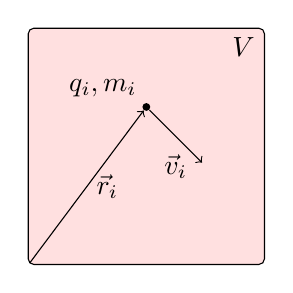
\begin{tikzpicture}
		\draw[fill=red!12!white,rounded corners=2pt] (0,0) rectangle (3,3);
		\node[fill=black,circle,inner sep=1pt, minimum size=1pt] (a) at (1.5,2) {};
		\draw[->] (0.02,0.02) -- node[right] {$ \vec{r}_i $} (a);
		\draw[->] (a) -- node[below=3pt] {$ \vec{v}_i $} ++(-45:1cm);
		\node[anchor=south east] at (a) {$q_i, m_i$};
		\node[anchor=north east] at (3,3) {$ V $};
	\end{tikzpicture}
	\vspace{5pt}
\end{minipage}%
\\
Zeitliche Änderung der Energie der Punktladungen durch die elektromagnetischen Felder:
\begin{align*}
\prd{}{t} W_{\tx{mat}} &= \prd{}{t} \sum_i \frac{m_i}{2} \vec{v}_i^2 = \sum_i \vec{v}_i \cdot m_i \cdot \prd{\vec{v}_i}{t} = \sum_i \vec{v}_i \cdot \vec{F}_i\\
&= \sum_i q_i \vec{v}_i \cdot \vec{E}(\vec{r}_i, t) + \sum_i q_i \ub{ \vec{v}_i \cdot (\vec{v}_i) \times \vec{B}(\vec{r}_i, t) }_{=0}\\
&= \sum_i q_i \vec{v}_i \cdot \vec{E}(\vec{r}_i, t)
\end{align*}
formale Kontinuierliche Beschreibung: $ \vec{j}(\vec{r},t) = \sum_i q_i \dot{\vec{r}}_i \delta(\vec{r} - \vec{r}_i(t)) $
\begin{equation*}
\rightarrow \quad \prd{}{t} W_{\tx{mat}} = \int_V \dd^3 r \ \vec{j}(\vec{r},t) \cdot \vec{E}(\vec{r},t)
\end{equation*}
Energiedichte $ w_{\tx{mat}} $: $ W_{\tx{mat}} = \int_V \dd^3 r \ w_{\tx{mat}} (\vec{r}) $
\begin{equation*}
\Rightarrow \quad \int_V \dd^3 r \ \vec{j} \cdot \vec{E} = \prd{}{t} \int_V \dd^3 r \ w_{\tx{mat}} = \int_V \dd^3 r \ \prt{}{t} w_{\tx{mat}}
\end{equation*}
\begin{equation*}
\Rightarrow \quad \int_V \dd^3 r \ \left(\prt{w_{\tx{mat}}}{t} - \vec{j} \cdot \vec{E} \right) = 0 \qquad \forall \ V
\end{equation*}
\begin{equation*}
\Rightarrow \quad \prt{w_{\tx{mat}}}{t} = \vec{j} \cdot \vec{E} \quad \widehat{=} \quad \tx{Leistungsdichte}
\end{equation*}
\begin{equation*}
[\vec{j}] [\vec{E}] = \frac{\tx{A}}{\tx{m}^2} \frac{\tx{V}}{\tx{m}} = \frac{\tx{W}}{\tx{m}^2}
\end{equation*}
Die gesamte Änderung der Energie der Materie im Volumen $ V $ ist dann:
\begin{equation*}
\prd{}{t} W_{\tx{mat}_V} = \int_V \dd^3 r \ \vec{j} \cdot \vec{E}
\end{equation*}
Außerdem gilt auch:
\begin{equation*}
\prd{}{t} W_{\tx{mat}} = - \prd{}{t} W_{\tx{feld}}
\end{equation*}
Wir wollen nun $ \vec{j} $ ersetzen und nutzen:
\begin{equation*}
\vec{j} = \vabla \times \vec{H} - \prt{\vec{D}}{t} \quad \Rightarrow \quad \vec{j} \cdot \vec{E} = \vec{E} \cdot (\vabla \times \vec{H}) - \vec{E} \cdot \prt{\vec{D}}{t}
\end{equation*}
$ \vec{E} $ mal der Rotation von $ \vec{H} $ können wir umformen als:
\begin{equation*}
\vabla \cdot (\vec{E} \times \vec{H}) = \vec{H} \cdot \ub{(\vabla \times \vec{E})}_{- \prt{\vec{B}}{t}} - \vec{E} \cdot (\vabla \times \vec{H})
\end{equation*}
\begin{equation*}
\rightarrow \quad  \vec{j} \cdot \vec{E} = - \vec{H} \cdot \prt{\vec{B}}{t} - \vec{E} \cdot \prt{\vec{D}}{t} - \vabla \cdot (\vec{E} \times \vec{H}) = \prt{}{t} w_{\tx{mat}}
\end{equation*}
\begin{equation*}
\Rightarrow \quad \prd{}{t} W_{\tx{mat}_V} = - \int_V \dd^3 r \ \left(\vec{H} \cdot \prt{\vec{B}}{t} + \vec{E} \cdot \prt{\vec{D}}{t} \right) - \int_V \dd^3 r \ \vabla \cdot (\vec{E} \times \vec{H}) = - \prd{}{t} W_{\tx{feld}}
\end{equation*}
Zur Vereinfachung und Interpretation: $ \vec{H} = \frac{1}{\mu} \vec{B} \quad \vec{D} = \epsilon \vec{E} \quad \epsilon, \mu \const $
\begin{equation*}
\vec{H} \cdot \prt{\vec{B}}{t} = \frac{1}{\mu} \vec{B} \cdot \prt{\vec{B}}{t} = \frac{1}{2} \frac{1}{\mu} \prt{}{t} (\vec{B} \cdot \vec{B}) = \frac{1}{2} \prt{}{t} (\vec{H} \cdot \vec{B})
\end{equation*}
\begin{equation*}
\vec{E} \cdot \prt{\vec{D}}{t} = \epsilon \vec{E} \cdot \prt{\vec{E}}{t} = \frac{\epsilon}{2} \prt{}{t} (\vec{E} \cdot \vec{E}) = \frac{1}{2} \prt{}{t} (\vec{E} \cdot \vec{D})
\end{equation*}
\begin{equation*}
\prd{}{t} W_{\tx{mat}_V} = - \prd{}{t} \frac{1}{2} \int_V \dd^3r \ (\vec{H} \cdot \vec{B} + \vec{E} \cdot \vec{D}) - \int_V \dd^3r \ \vabla \cdot (\vec{E} \times \vec{H})
\end{equation*}
\textbf{Elektrostatik:}
\begin{equation*}
w_{\tx{el}} = \frac{\epsilon_0}{2} \vec{E}^2 \quad (\tx{Vakuum}) \qquad w_{\tx{el}} = \frac{1}{2} \vec{E} \cdot \vec{D} \quad (\tx{Medium})
\end{equation*}
\textbf{Magnetostatik:}
\begin{equation*}
w_{\tx{mag}} = \frac{1}{2 \mu_0} \vec{B}^2 \quad (\tx{Vakuum}) \qquad w_{\tx{mag}} = \frac{1}{2} \vec{H} \cdot \vec{B} \quad (\tx{Medium})
\end{equation*}
Energie des elektromagnetischen Feldes:
\begin{equation*}
\frac{1}{2} \int_V \dd^3 r \ (\vec{H} \cdot \vec{B} + \vec{E} \cdot \vec{D}) = W_{\tx{em}_V}
\end{equation*}
Energiedichte:
\begin{equation*}
w_{\tx{em}} = \frac{1}{2} (\vec{H} \cdot \vec{B} + \vec{E} \cdot \vec{D})
\end{equation*}
\begin{equation*}
\prd{}{t} W_{\tx{mat}_V} = - \prd{}{t} W_{\tx{em}_V} - \ub{\int_V \dd^3 r \ \vabla \cdot (\vec{E} \times \vec{H})}_{\mathclap{\substack{\tx{Energie, die aus } V \\ \tx{abfließt (Strahlung)}}}}
\end{equation*}
\begin{equation*}
\vec{S}(\vec{r},t) = \vec{E} \times \vec{H} \qquad \tx{\textbf{Pointing-Vektor}}
\end{equation*}
\begin{equation*}
\int_V \dd^3 r \ \vabla \vec{S} = \int_{\partial V} \dd\vec{f}  \cdot \vec{S}
\end{equation*}
\begin{equation*}
[\vec{S}] = [\vec{E}] [\vec{H}] = \frac{\tx{V}}{\tx{m}} \frac{\tx{A}}{\tx{m}} = \frac{\tx{W}}{\tx{m}^2} = \frac{\tx{J}}{\tx{m}^2 \tx{s}} = \frac{\tx{Energie}}{\tx{Fläche } \cdot \tx{ Zeit}}
\end{equation*}
$ \vec{S}: $ \textbf{Energiestromdichte}\\
\begin{minipage}{.8\linewidth}
	% Hier fehlt ein Text von Kim:
	$$ \int_{\partial V} \dd \vec{f} \cdot \vec{S} $$
	Energiestrom des EM-Feldes durch die Fläche $ \partial V $.
\end{minipage}%
\begin{minipage}{.2\linewidth}
	\flushright
	%t2:
	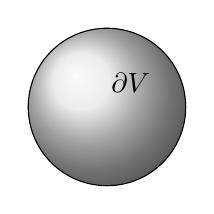
\begin{tikzpicture}
	\draw[shade, ball color=gray!20!white] (0,0) circle (1cm);
	\node at (.3,.3) {$ \partial V $};
	\end{tikzpicture}
\end{minipage}%

\subsubsection{Energiebilanz}

\begin{equation*}
\ub{\prd{}{t} W_{\tx{mat} _V}}_{\mathclap{\substack{\tx{an Ladungen} \\ \tx{in } V \tx{ verrichtete} \\ \tx{Arbeit}}}} \ \ + \ \ \ub{\prd{}{t} W_{\tx{em}_V}}_{\mathclap{\substack{\tx{Änderung der} \\ \tx{EM Feldenergie} \\ \tx{in } V}}} \ = \ \ub{- \int_{\partial V} \dd \vec{f} \cdot \vec{S}}_{\mathclap{\substack{\tx{Fluss der EM} \\ \tx{Feldenergie aus } V}}}
\end{equation*}
%
%
%

\pagebreak

%
%
%
\noindent
\emph{Bemerkungen:}
\begin{enumerate}[i)]
	\item abgeschlossenes System (ohne Energiestromdichte ach außen) z.B. $ \mathbb{R}^3 $
	\begin{equation*}
	\int_{\partial V} \dd \vec{f} \cdot \vec{S} \rightarrow 0
	\end{equation*}
	\item Gebiet ohne Ladungen und Ströme $ \rho = \vec{j} = 0 \ \ \tx{in} V $. $ w_{\tx{mat}} = \vec{j} \cdot \vec{E} = 0 $
	\begin{equation*}
	\prd{}{t} W_{\tx{mat}_V} = - \int_{\partial V} \dd \vec{f} \cdot \vec{S}
	\end{equation*}
	\item differentielle Form:
	\begin{equation*}
	\int_V \dd^3 r \ \left[\prt{w_{\tx{em}}}{t} + \vabla \cdot \vec{S} + \vec{j} \cdot \vec{E}\right] = 0
	\end{equation*}
	\frbox{Poyntigsches Theorem}{
	\begin{equation*}
	\rightarrow \quad \prt{w_{\tx{em}}}{t} + \prt{w_{\tx{mat}}}{t} + \vabla \cdot \vec{S} = 0
	\end{equation*}}
	oder auch: \textbf{Kontinuitätsgleichung für Energie}
	\begin{equation*}
	\prt{}{t} w + \vabla \cdot \vec{S} = 0
	\end{equation*}
	Analogie:
	\begin{equation*}
	\prt{\rho}{t} + \vabla \cdot \vec{j} = 0
	\end{equation*}
	\item \textbf{Poynting-Vektor}
	\begin{equation*}
	\vec{S} = \vec{E} \times \vec{H} \quad \tx{Energiestromdichte}
	\end{equation*}
	\textbf{Beachte:} Nur $ \vabla \cdot \vec{S} $ oder $ \int_{\partial V} \dd \vec{f} \cdot \vec{S} $ haben physikalische Bedeutung.\\[5pt]
	$ \vec{S} \to \vec{S} + \vabla \times \vec{G} $\\
	$ \vec{S} \neq 0 $, aber kein Energiestrom:
	\begin{equation*}
	\vec{E} = E \vec{e}_x \quad \vec{H} = H \vec{e}_y \qquad E,H \const
	\end{equation*}
	\begin{equation*}
	\vec{S} = \vec{E} \times \vec{H} = E H \vec{e}_z \neq 0
	\end{equation*}
	aber: $ \vabla \cdot \vec{S} = 0  \quad \rightarrow $ \textbf{kein Beitrag !}
\end{enumerate}
\emph{Beispiel:} \textbf{Energietransport in el./mag. Wellen im Vakuum}
\begin{center}
	%t3:
	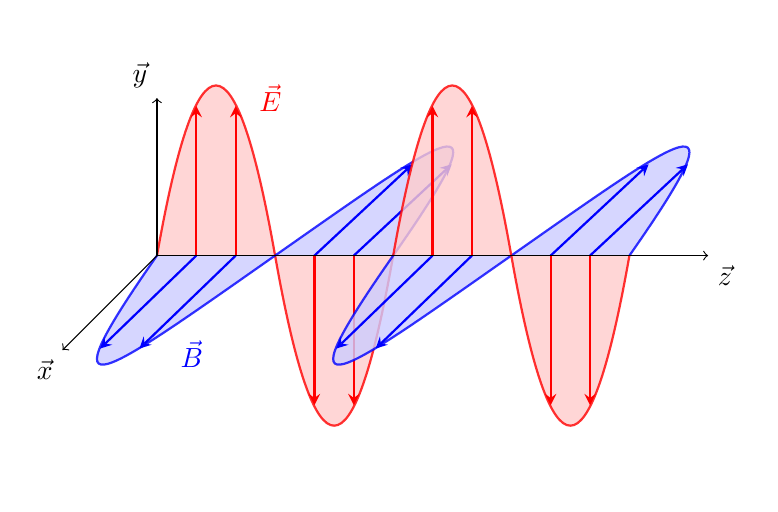
\begin{tikzpicture}%[>=stealth]
		% E
		\draw[red,thick,looseness=5,fill=red!20!white,opacity=.8] (0,0) to[out=80,in=100] (1.5,0) to[out=-80,in=-100] (3,0);
		\foreach \z in {.5,1}
		\draw[thick,red,->,>=stealth] (\z,0) -- ++(0,1.9);
		\foreach \z in {2,2.5}
		\draw[thick,red,->,>=stealth] (\z,0) -- ++(0,-1.9);
		% B
		\draw[blue,thick,looseness=4.5,fill=blue!20!white,opacity=.8] (0,0) to[out=-125,in=-145] (1.5,0) to[out=35,in=55] (3,0) to[out=-125,in=-145] (4.5,0) to[out=35,in=55] (6,0);
		\foreach \z in {.5,1,3.5,4}
		\draw[thick,blue,->,>=stealth] (\z,0) -- ++(-136:1.7cm);
		\foreach \z in {2,2.5,5,5.5}
		\draw[thick,blue,->,>=stealth] (\z,0) -- ++(43:1.7cm);
		% rest E
		\draw[red,thick,looseness=5,fill=red!20!white,opacity=.8] (3,0) to[out=80,in=100] (4.5,0) to[out=-80,in=-100] (6,0);
		\foreach \z in {3.5,4}
		\draw[thick,red,->,>=stealth] (\z,0) -- ++(0,1.9);
		\foreach \z in {5,5.5}
		\draw[thick,red,->,>=stealth] (\z,0) -- ++(0,-1.9);
		% koordinatensystem
		\draw[->] (0,0) -- (0,2) node[anchor=south east] {$ \vec{y} $};
		\draw[->] (0,0) -- (-1.2,-1.2) node[anchor=north east] {$ \vec{x} $};
		\draw[->] (0,0) -- (7,0) node[anchor=north west] {$ \vec{z} $};
		\node (e) at (1.5,2) {\color{red} $ \vec{E} $ \color{black}};
		\node (b) at (.5,-1.25) {\color{blue} $ \vec{B} $ \color{black}};
	\end{tikzpicture}
\end{center}
ebene Welle:
\begin{align*}
\vec{E} &= E_0 \cos(kz - \omega t) \vec{e}_x \\
\vec{B} &= \frac{E_0}{c} \cos(kz - \omega t) \vec{e}_y
\end{align*}
\begin{equation*}
\frac{\omega}{k} = c \qquad \lambda = \frac{2 \pi}{k}
\end{equation*}
mit $ c^2 = \frac{1}{\epsilon_0 \mu_0} $\\
\begin{minipage}{.7\linewidth}
	\begin{align*}
	\vec{S} &= \vec{E} \times \vec{H} = \frac{1}{\mu_0} \vec{E} \times \vec{B} = \frac{1}{\mu_0} \frac{E_0^2}{c} \cos^2(kz - \omega t) \vec{e}_z\\
	&= c \epsilon_0 E_0^2 \cos^2(kz - \omega t) \vec{e}_z
	\end{align*}
\end{minipage}%
\begin{minipage}{.3\linewidth}
	\flushright
	%t4:
	\begin{tikzpicture}
		\draw[thick,->] (0,0) -- (0,1.5) node[anchor=south east] {$ \vec{E} $};
		\draw[thick,->] (0,0) -- (1.5,0) node[anchor=north west] {$ \vec{S} $};
		\draw[thick,->] (0,0) -- (-.75,-.75) node[anchor=north east] {$ \vec{B} $};
	\end{tikzpicture}
\end{minipage}%
\\
\textbf{explizite Energiebilanz:}
\begin{equation*}
\prt{}{t} (\equalto{w_{\tx{mat}}}{0} + w_{\tx{em}}) = - \vabla \cdot \vec{S}
\end{equation*}
\begin{align*}
w_{\tx{em}} &= \frac{1}{2} (\vec{E} \cdot \vec{D} + \vec{H} \cdot \vec{B}) = \frac{1}{2} (\epsilon_0 \vec{E}^2 + \frac{1}{\mu_0} \vec{B}^2) \\
&= \frac{\epsilon_0}{2} (\vec{E}^2 + c^2 \vec{B}^2) = \epsilon_0 E_0^2 \cos^2(kz - \omega t)
\end{align*}
\begin{equation*}
\prt{}{t} w_{\tx{em}} = 2 \omega \epsilon_0 E_0^2 \cos(\dots) \sin(\dots)
\end{equation*}
\begin{equation*}
\vabla \cdot \vec{S} = \prt{S}{z} = - 2 \ub{kc}_{= \omega} \epsilon_0 E_0^2 \cos(\dots) \sin(\dots)
\end{equation*}

\subsection{Impuls des EM-Feldes - Maxwellscher Spannungstensor}

Wir betrachten ein System von Punktladungen: $ q_i, m_i, \vec{r}_i, \vec{v}_i $
Impuls: $ \vec{p_i} = m_i \vec{v}_i $
\begin{equation*}
\vec{D} = \epsilon \vec{E} \qquad \vec{B} = \mu \vec{H}
\end{equation*}
Die zeitliche Änderung des gesamten Impulses der Teilchen durch EM-Felder:
\begin{align*}
\prd{}{t} \vec{P}_{\tx{mat}} &= \prd{}{t} \sum_i \vec{p_i} = \sum_i \prd{}{t} \vec{p}_i\\
&= \sum_i \vec{F}_i = \sum_i q_i \left(\vec{E}(\vec{r}_i, t) + \vec{v}_i \times \vec{B}(\vec{r}_i, t)\right)
\end{align*}
$ \rightarrow $ Kontinuierliche Beschreibung:
\begin{align*}
\rho(\vec{r},t) &= \sum_i q_i \delta(\vec{r} - \vec{r}_i(t))\\
\vec{j}(\vec{r},t) &= \sum_i q_i \vec{v}_i \delta(\vec{r} - \vec{r}_i(t))
\end{align*}
\begin{equation*}
\rightarrow \quad \prd{}{t} \vec{P}_{\tx{mat}} = \int_V \dd^3 r \ \ub{\left(\rho \vec{E}(\vec{r},t) + \vec{j} \times \vec{B}(\vec{r},t)\right)}_{\tx{Kraftdichte}}
\end{equation*}
$ \rho = \vabla \cdot \vec{D} \quad \vec{j} = \vabla \times \vec{H} - \prt{\vec{D}}{t} $
\begin{equation*}
\Rightarrow \quad \rho \vec{E} + \vec{j} \times \vec{B} = - \prt{}{t} (\vec{D} \times \vec{B}) + \sum_{i,k=1}^{3} \prt{T_{ik}}{x_k} \vec{e}_i
\end{equation*}
\textbf{Maxwellscher Spannungstensor:}\\[5pt]
Symmetrischer Tensor 2. Stufe:
\begin{equation*}
T_{ik} = \epsilon E_i E_k - \frac{1}{\mu} B_i B_k - \frac{1}{2} \delta_{ik}(\epsilon \vec{E}^2 - \frac{1}{\mu} \vec{B}^2)
\end{equation*}
physikalisch: \textbf{Impulsstromdichte}

\subsubsection{Impulsbilanz}

\begin{equation*}
\prd{}{t} \vec{P}_{\tx{mat}_V} + \prd{}{t} \int_V \dd^3 r \ (\vec{D} \times \vec{B}) = \sum_{i=1}^{3} \ub{\Bigg(\int_{V} \dd^3 r\ \ob{\sum_{k=1}^{3} \prt{T_{ik}}{x_k}}^{= \vabla \cdot \vec{T}_i} \vec{e}_i \Bigg)}_{= \int_{\partial V} \dd \vec{f} \cdot \vec{T}_i}
\end{equation*}
Die $ i $-te Zeile dieser $ 3 \times 3 $-Matrix wäre als Vektor: $ \vec{T}_i = (T_{i1}, T_{i2}, T_{i3}) $
\begin{equation*}
\ub{\prd{}{t} \vec{P}_{\tx{mat}_V}}_{\mathclap{\substack{\tx{Änderung des} \\ \tx{Impulses} \\ \tx{der Teilchen}}}} + \ub{\prd{}{t} \int_V \dd^3 r (\vec{D} \times \vec{B})}_{\mathclap{\substack{\tx{Änderug des} \\ \tx{Impulses des} \\ \tx{EM-Feldes} \\ \tx{in } V}}} = \ub{\sum_{i = 1}^{3} \int_{\partial V} \dd \vec{f} \cdot \vec{T}_i}_{\mathclap{\substack{\tx{Impulsfluss} \\ \tx{des EM-Feldes} \\ \tx{aus } V}}}
\end{equation*}

%Vorlesung 20.12.18 (4 Days until christmas)

\begin{comment}
\begin{align*}
\prd{}{t} P_{\tx{mat}_V} &= \sum_i \vec{F}_i = \sum_i q_i (\vec{E}(\vec{r},t) + \vec{v}_i \times \vec{B}(\vec{r}_i,t)\\
&= \int_V \dd^3r (\rho \vec{E} + \vec{j} \times \vec{B})
\end{align*}
\begin{equation*}
\Rightarrow \prd{}{t} P_{\tx{mat}_V} + \prd{}{t} \int_V\dd^3 r(\vec{D} \times \vec{B}) = \sum_{i=1}^{3} \ub{\int_V \dd^2 r \sum_{k=1}^{3} \prt{T_{ik}}{x_k} \vec{e}_i}_{= \int_{\partial V} \dd\vec{f} \cdot \vec{T}_i \vec{e}_i}
\end{equation*}
\end{comment}

\noindent
differentiell:
\begin{equation*}
\rho \vec{E} + \vec{j} \times \vec{B} + \prt{}{t} (\vec{D} \times \vec{B}) = \sum_i (\vabla \cdot \vec{T}_i) \vec{e}_i
\end{equation*}
\begin{enumerate}[i)]
	\item \textbf{Impuls des EM-Feldes}
	\begin{equation*}
	P_{\tx{em}_V} = \int_V \dd^3 r \ub{(\vec{D} \times \vec{B})}_{=\vec{g}}
	\end{equation*}
	$ \vec{g} \defeq $ Impulsdichte\\
	$ \vec{D} = \epsilon \vec{E} \qquad \vec{B} = \mu \vec{H} $
	\begin{equation*}
	\rightarrow \quad \vec{g} = \epsilon \mu \ub{\vec{E} \times \vec{H}}_{=\vec{S}} = \epsilon_r \mu_r \ub{\epsilon_0 \mu_0}_{= \frac{1}{c^2}} \vec{S} = \epsilon_r \mu_r \frac{1}{c^2} \vec{S}
	\end{equation*}
	$ \left[\frac{1}{c^2} \vec{S}\right] = \frac{\tx{Impuls}}{\tx{Volumen}} $\\[10pt]
	Impulsdichte einer ebenen Wellen:
	\begin{align*}
	\vec{E} &= E_0 \cos\left(kz - \omega t\right) \vec{e}_x\\
	\vec{B} &= \frac{E_0}{c} \cos\left(kz - \omega t\right) \vec{e}_y\\
	\vec{S} &= \vec{E} \times \vec{H} = c \epsilon_0 E_0^2 \cos^2(kz - \omega t) \vec{e}_z\\
	\vec{g} &= \frac{\epsilon_0}{c} E_0^2 \cos^2(kz - \omega t) \vec{e}_z
	\end{align*}
	\item \textbf{Maxwellscher Spannungstensor - Impulsdichte}
	\begin{equation*}
	T_{ik} = \epsilon E_i E-k + \frac{1}{\mu} B_i B_k - \frac{1}{2} \delta_{ik} \left(\epsilon \vec{E}^2 + \frac{1}{\mu} \vec{B^2}\right)
	\end{equation*}
	\begin{equation*}
	\prd{}{t} \left(\vec{P}_{\tx{mat}_V} + \vec{P}_{\tx{em}_V}\right) = \sum_i \left(\int_V \dd\vec{f} \cdot \vec{T}_i \right)\vec{e}_i
	\end{equation*}
	Analogie: Energiebilanz
	\begin{equation*}
	\prd{}{t} \left(W_{\tx{mat}_V} + W_{\tx{em}_V}\right) = - \int_{\partial V} \dd \vec{f} \cdot \vec{S}
	\end{equation*}
	$ \Rightarrow - \vec{T}_i $ Impulsstromstärke zu $ P_i $\\
	$ \left[T_{ik}\right] = \frac{\tx{Impuls}}{\tx{Fläche } \cdot \tx{ Zeit}} $\\[10pt]
	$ T_{ik} : $ Berechnung von Kräften auf geladene materielle Körper im EM-Feld.\\
	\begin{minipage}{.6\linewidth}
		\begin{align*}
		\prd{}{t} \vec{P} &= \sum_i \int_{\partial V} \dd \vec{f} \cdot \vec{T}_i \vec{e}_i\\
		&= \sum_{i=1}^{3} \ub{\left(\prd{}{t} P_i\right)}_{\mathclap{\tx{Kraft } \vec{K} , K_i}} \vec{e}_i
		\end{align*}
		\begin{equation*}
		\Rightarrow \quad \dd K_i = (\vec{n} \cdot \vec{T}_i) \dd f
		\end{equation*}
		$ \dd \vec{f} = \vec{n} \dd f $
		\begin{equation*}
		\Rightarrow \quad \left[\frac{\dd K_i}{\dd f}\right] = \frac{\tx{Kraft}}{\tx{Fläche}} = \tx{ Druck}
		\end{equation*}
	\end{minipage}%
	\begin{minipage}{.4\linewidth}
		\flushright
		%t1:
		\begin{tikzpicture}
			\pic at (0,0) {annotated cuboid={width=7,height=20,depth=20}};
			\draw[thick,->] (.4,-.6) -- ++(1,0) node[right] {$ \dd \vec{f} $};
			% \draw (0,0) -- (.78,-1.23); % diagonale
			\draw (.45,-1) to[out=-45,in=100] (1,-2) node[below] {$ \vec{P} $};
			% waves
			\coordinate (a) at (-2.5,-.6);
			\draw[red!90!white,thick,->] (a) -- ++(60:2.5cm);
			\draw[red!90!white,thick,->] ($ (a) + (-60:.4cm) $) -- ++(60:2.5cm);
			\draw[blue!90!white,thick,->] (a) -- ++(-60:2.5cm);
			\draw[blue!90!white,thick,->] ($ (a) + (60:.4cm) $) -- ++(-60:2.5cm);
			\node[red!90!white] at ($ (a) + (55:2.8cm) $) {$ \vec{E} $};
			\node[blue!90!white] at ($ (a) + (-55:2.8cm) $) {$ \vec{B} $};
		\end{tikzpicture}
	\end{minipage}%
	\\[10pt]
\end{enumerate}
\emph{Beispiel:} \textbf{Plattenkondensator}\\
\begin{minipage}{.6\linewidth}
	\begin{equation*}
	\vec{E} = \casess{E \vec{e}_x}{\tx{innen}}{0}{\tx{außen}} \qquad \vec{B} = 0
	\end{equation*}
\end{minipage}%
\begin{minipage}{.4\linewidth}
	\flushright
	%t2:
	\begin{tikzpicture}
	\draw[very thick] (-1.3,-2) -- (-1.3,2) node[above] {$ \sigma $};
	\draw[very thick] (1.3,-2) -- (1.3,2) node[above] {$ - \sigma $};
	\draw[->] (0,-2.5) -- ++(2,0) node[right] {$ x $};
	\draw ($ (0,-2.5) + (0,.1) $) -- ($ (0,-2.5) + (0,-.1) $);
	\foreach \y in {-1.8,-.6,.6,1.8}
	\draw[->] (-1.1,\y) -- (1.1,\y);
	\foreach \y in {-1.8,-.6,.6,1.8}
	%\node at (-1.8,\y) {$ + $};
	\draw[fill = white!20!red] (-1.6,\y) circle (.2cm) node[] {$ \color{white} + \color{white} $};
	\foreach \y in {-1.8,-.6,.6,1.8}
	%\node at (1.8,\y) {$ - $};
	\draw[fill = white!20!blue] (1.6,\y) circle (.2cm) node[] {$ \color{white} - \color{white} $};
	\node[above] at (0,2) {$ \vec{E} $};
	\end{tikzpicture}
\end{minipage}%
\\
Krafttensor innen:
\begin{equation*}
T_{ik} = \ \ub{\epsilon E_i E_k}_{\mathclap{= \epsilon_0 E^2 \delta_{ix} \delta_{kx}}} \ + \ub{\frac{1}{\mu} B_i B_k}_{=0} - \frac{1}{2} \delta_{ik} \bigg(\ub{\epsilon \vec{E}^2}_{\epsilon_0 E^2} + \ub{\frac{1}{\mu} \vec{B^2}}_{= 0}\bigg)
\end{equation*}
Krafttensor außen:
\begin{equation*}
T_{ik} = 0
\end{equation*}
\vspace{5pt}
\begin{equation*}
T_{xx} = \frac{\epsilon_0}{2} E^2 \qquad T_{yy} = T_{zz} = - \frac{\epsilon_0}{2} E^2 \qquad \tx{sonst } = 0
\end{equation*}
\begin{equation*}
T_{ik} = \frac{\epsilon_0}{2} E^2 \begin{pmatrix}
1 & 0 & 0\\
0 & -1 & 0\\
0 & 0 & -1
\end{pmatrix}
\end{equation*}
Kraft in x-Richtung:
\begin{equation*}
K_x = \int_{\partial V} \dd\vec{f} \cdot \ub{\vec{T}_x}_{\mathclap{= (T_{xx},T_{xy},T_{xz}) = \frac{\epsilon_0}{2} E^2 \vec{e}_x}} = \int_{\partial V} \dd \vec{f} \cdot \frac{\epsilon_0}{2} E^2 \vec{e}_x
\end{equation*}
\begin{minipage}{.6\linewidth}
	$ \dd \vec{f} = \dd y \dd z \vec{e}_x $
	\begin{equation*}
	K_x = \int_{F_x} \dd f \frac{\epsilon_0}{2} E^2 = \frac{\epsilon_0}{2} E^2 F_x
	\end{equation*}
	$\rightarrow \quad \frac{\tx{Kraft}}{\tx{Fläche}} : \quad \frac{K_x}{F_x} = \frac{\epsilon_0}{2} E^2 = \frac{\sigma^2}{2 \epsilon_0}$
	\begin{equation*}
	\vec{K} = (K_x,0,0)
	\end{equation*}
\end{minipage}%
\begin{minipage}{.4\linewidth}
	\flushright
	%t3:
	\begin{tikzpicture}
	\foreach \x\y in {-.1/-.5, -.1/-1.35, -.1/-2.2}
	\draw[shade, ball color = red] (\x,\y) circle (.2cm) node[] {$ \color{white} + \color{white} $};
	\pic at (0,0) {annotated cuboid={width=5,height=30,depth=30}};
	\draw (0,.2) to[out=90,in=-40] (-.5,1) node[left] {$ V $};
	\foreach \x\y in {.7/.3, .7/-.55, .7/-1.4}
	\draw[shade, ball color = red] (\x,\y) circle (.2cm) node[] {$ \color{white} + \color{white} $};
	% diagonale besser aber nicht perfekt
	% \draw (0,0) -- ($ (0,-3) +({sin(45) * 1.65},{cos(45) * 1.65}) $);
	\draw[thick, ->] (.6,-1) -- ++(1,0) node[right] {$ \dd\vec{f}_x $};
	\draw (.5,-1.8) -- ++(-30:1cm) node[anchor=north west] {$ \substack{\tx{nur diese Fläche ($F_x$)} \\ \tx{trägt bei}} $};
	\end{tikzpicture}
\end{minipage}%

\section{Elektromagnetische Wellen}

\subsection{Maxwell-Gleichungen in einem Isolator - Homogene Wellengleichung}

\begin{equation*}
\rho_f = 0 = \vec{j}_f
\end{equation*}
$ \vec{D} = \epsilon \vec{E} \quad \vec{B} = \mu \vec{H} $
\begin{equation*}
\vabla \cdot \vec{E} = 0 \qquad \qquad \vabla \cdot \vec{B} = 0
\end{equation*}
\begin{equation*}
\quad \, \vabla \times \vec{E} + \prt{\vec{B}}{t} = 0 \qquad \qquad \vabla \times \vec{B} - \epsilon \mu \prt{\vec{E}}{t} = 0
\end{equation*}
\begin{equation*}
0 = \ub{\vabla \times \left(\vabla \times \vec{E}\right)}_{\vabla\ub{(\vabla \cdot \vec{E})}_{= 0} - \Delta \vec{E}} + \prt{}{t} \ub{\vabla \times \vec{B}}_{= \epsilon \mu \prt{\vec{E}}{t}} = - \Delta \vec{E} + \epsilon \mu \prt{^2 \vec{E}}{t^2}
\end{equation*}
\begin{equation*}
\Rightarrow \quad \Delta \vec{E} - \epsilon \mu \prt{^2 \vec{E}}{t^2} = 0
\end{equation*}
$ \epsilon \mu = \epsilon_r \mu_r \epsilon_0 \mu_0 = \frac{\epsilon_r \mu_r}{c^2} \qquad n = \sqrt{\epsilon_r \mu_r} $\\[5pt]
$ n $ ist der Brechungsindex des betrachteten Materials $ v = \frac{c}{n} $ die Geschwindigkeit der EM-Welle in diesem Material.
\begin{equation*}
\Rightarrow \quad \rmbox{\Delta \vec{E} - \frac{n^2}{c^2} \prt{^2 \vec{E}}{t^2} = 0}
\end{equation*}
außerdem gilt:
\begin{align*}
0 &= \ub{\vabla \times (\vabla \times \vec{B})}_{\vabla \ub{(\vabla \cdot \vec{B})}_{= 0} - \Delta \vec{B}} - \epsilon \mu \prt{}{t} \ub{\vabla \times \vec{E}}_{= - \prt{\vec{B}}{t}}
\end{align*}
\begin{equation*}
\Rightarrow \quad \rmbox{\Delta \vec{B} - \frac{n^2}{c^2} \prt{^2 \vec{B}}{t^2} = 0}
\end{equation*}
homogene Wellengleichung ($ \Psi(\vec{r},t) $)
\begin{equation*}
\Delta \Psi - \frac{n^2}{c^2} \prt{^2 \Psi}{t^2} = 0
\end{equation*}
\begin{equation*}
\Psi = E_x, E_y, E_z, B_x, B_y, B_z
\end{equation*}

% Neue Vorlesung 7.01.19

\bbb{Wiederholung}{
Maxwell-Gl für Isolator: $ \rho_f = 0 = \vec{j}_f \quad \vec{D} = \epsilon \vec{E} \quad \vec{H} = \frac{1}{\mu} \vec{B} $
\begin{equation*}
\vabla \cdot \vec{E} = 0 \qquad \qquad \vabla \cdot \vec{B} = 0
\end{equation*}
\begin{equation*}
\quad \, \vabla \times \vec{E} + \prt{\vec{B}}{t} = 0 \qquad \qquad \vabla \times \vec{B} - \epsilon \mu \prt{\vec{E}}{t} = 0
\end{equation*}
$ \epsilon \mu = \epsilon_r \mu_r \epsilon_0 \mu_0 = \frac{\epsilon_r \mu_r}{c^2} = \rmbox{ \frac{n^2}{c^2} = \frac{1}{v^2} } \qquad n = \sqrt{\epsilon_r \mu_r} $
homogene Wellengleichungen:
\begin{equation*}
\Rightarrow \quad \rmbox{\Delta \vec{E} - \frac{n^2}{c^2} \prt{^2 \vec{E}}{t^2} = 0} \qquad 
\Rightarrow \quad \rmbox{\Delta \vec{B} - \frac{n^2}{c^2} \prt{^2 \vec{B}}{t^2} = 0}
\end{equation*}
für jede Komponente von $ \vec{E} $ und $ \vec{B} $ gilt:
\begin{equation*}
\Delta \Psi - \frac{1}{v^2} \prt{^2 \Psi}{t^2} = 0
\end{equation*}
\lcom{Aus den Maxwell-Gleichungen ist aber zu sehen, dass $ \vec{E} $ und $ \vec{B} $-Felder \textbf{nicht} unabhängig voneinander sind.}
}
\subsection{Homogene Wellengleichung für skalare Funktion in einer Raumdimension}
\begin{equation*}
\Psi(x,t) \qquad \prt{^2 \Psi}{x^2} - \frac{1}{v^2} \prt{^2 \Psi}{t^2} = 0
\end{equation*}
Funktionen der Form $ \Psi_{\pm}(x,t) = f(x \pm vt) $ erfüllen die Wellengleichung.\\
\begin{equation*}
\prt{^2}{x^2} f(x \pm vt) = f''(x \pm vt)
\end{equation*}
\begin{equation*}
\prt{^2 f}{t^2} = \prt{}{t} f' (x \pm vt) \cdot (\pm v) = v^2 f'' (x \pm vt)
\end{equation*}
Wie sehen diese Lösungen nun aus?
\begin{equation*}
\Psi_-(x,t) = f(x - vt)
\end{equation*}
$ \Psi_-(x,0) = f(x) \ \leftarrow t = 0 $\\
\begin{center}
	%t1:
	%\begin{tikzpicture}
	%\draw [domain=-4:4, samples=100,scale=.3] plot (\x, {5*exp(-(\x)^(2)*0.25});
	%\end{tikzpicture}
	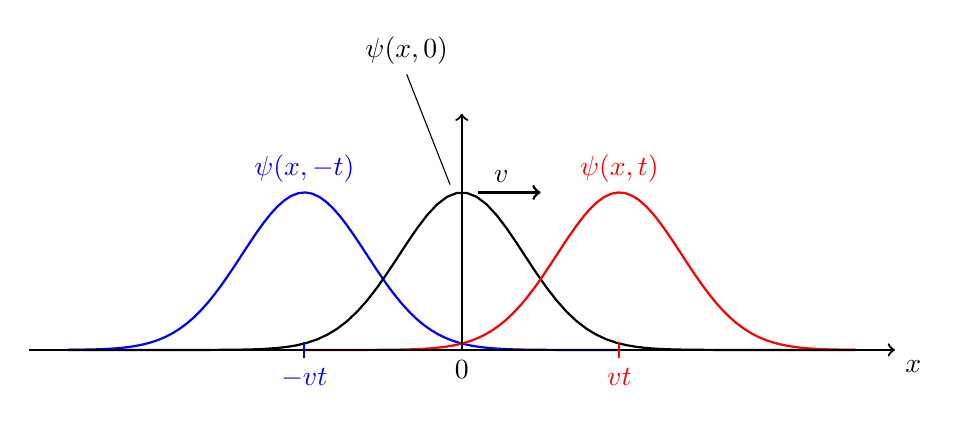
\begin{tikzpicture}
		%rechts
		%\draw[red,line width=1] (4,0) .. controls (3.2,0.2) and (2.8,1.8) .. (2,2);
		%\draw[red,line width=1] (0,0) .. controls (0.8,0.2) and (1.2,1.8) .. (2,2);
		\draw[domain=-5:2, samples=80, blue, thick] plot (\x, {2*exp(-(\x + 2)^(2)*0.8});
		%mitte
		%\draw[line width=1] (-2,0) .. controls (-1.2,0.2) and (-0.8,1.8) .. (0,2);
		%\draw[line width=1] (2,0) .. controls (1.2,0.2) and (0.8,1.8) .. (0,2);
		\draw[domain=-5:5, samples=80, thick] plot (\x, {2*exp(-(\x + 0)^(2)*0.8});
		%links
		%\draw[blue,line width=1] (-4,0) .. controls (-3.2,0.2) and (-2.8,1.8) .. (-2,2);
		%\draw[blue,line width=1] (0,0) .. controls (-0.8,0.2) and (-1.2,1.8) .. (-2,2);
		\draw[domain=-2:5, samples=80, red, thick] plot (\x, {2*exp(-(\x - 2)^(2)*0.8});
		%achsen
		\draw[thick, <-] (5.5,0) node[anchor=north west] {$x$}-- (-5.5,0);
		\draw[thick, ->] (0,0) node[below] {$0$} -- (0,3); % node[anchor=south east] {$y$};
		%
		\draw[line width=1,->] (0.2,2) -- (1,2);
		\draw[dotted] (0.5,2) node[above] {$v$};
		\draw[thick, red] (2,0.1) -- (2,-0.1) node[below] {$vt$};
		\draw[thick, blue] (-2,0.1) -- (-2,-0.1) node[below] {$-vt$};
		\draw[dotted] (2,2) node[red,above] {$\psi (x,t)$};
		\draw[dotted] (-2,2) node[blue,above] {$\psi (x,-t)$};
		\draw (-.7,3.5) node[above] {$\psi (x,0)$} -- (-0.15,2.1);
	\end{tikzpicture}
\end{center}
$ t > 0: \quad \Psi_-(x,t) = f(x - vt) $\\
$ \Psi_+(x,t) = f(x + vt) $\\[5pt]
Wellengleichungen sind linear $ \Rightarrow $ Linearkombinationen von Lösungen sind wieder Lösungen.
\begin{align*}
\Psi(x,t) &= a_1 \Psi_1(x,t) + a_2 \Psi_2(x,t)\\
&= a_1 f_1(x+vt) + a_2 f_2(x-vt)
\end{align*}
\lcom{Im allgemeinen muss es aber nicht sein, dass eine Welle bei Zeittransformationen ihre Form beibehält!}\\
\begin{center}
	%t2:
	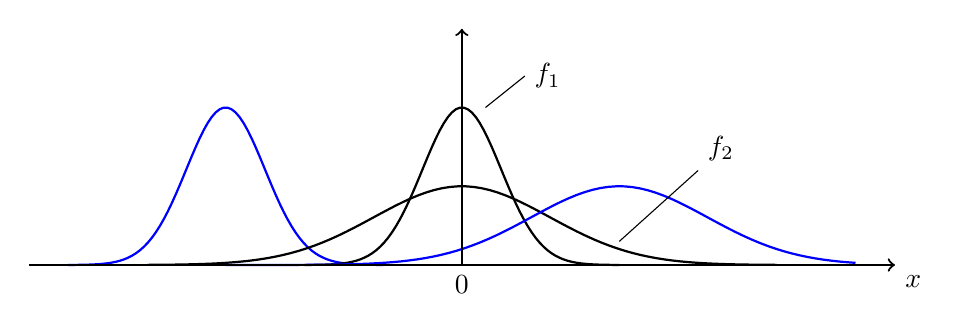
\begin{tikzpicture}
		%\draw[line width=1,blue] (-4.5,0) .. controls (-3.3,0.1) and (-3.8,1.8) .. (-3,2);
		%\draw[line width=1,blue] (-1.5,0) .. controls (-2.7,0.1) and (-2.2,1.8) .. (-3,2);
		\draw[domain=-5:-1, samples=80, blue, thick] plot (\x, {2*exp(-(\x + 3)^(2)*2});
		%
		%\draw[line width=1] (-1.5,0) .. controls (-0.3,0.1) and (-0.8,1.8) .. (0,2);
		%\draw[line width=1] (1.5,0) .. controls (0.3,0.1) and (0.8,1.8) .. (0,2);
		\draw[domain=-2:2, samples=80, thick] plot (\x, {2*exp(-(\x + 0)^(2)*2});
		%
		%\draw[line width=1] (-3.5,0) .. controls (-1.2,0) and (-1.1,0.9) .. (0,1);
		%\draw[line width=1] (3.5,0) .. controls (1.2,0) and (1.1,0.9) .. (0,1);
		\draw[domain=-4:4, samples=80, thick] plot (\x, {1*exp(-(\x + 0)^(2)*.4});
		%
		%\draw[line width=1,blue] (-1.5,0) .. controls (0.8,0) and (0.9,0.9) .. (2,1);
		%\draw[line width=1,blue] (5.5,0) .. controls (3.2,0) and (3.1,0.9) .. (2,1);
		\draw[domain=-3:5, samples=80, blue, thick] plot (\x, {1*exp(-(\x - 2)^(2)*.4});
		%achsen
		\draw[thick, <-] (5.5,0) node[anchor=north west] {$x$}-- (-5.5,0);
		\draw[thick, ->] (0,0) node[below] {$0$} -- (0,3); % node[anchor=south east] {$y$};
		%
		\draw (2,.3) -- (3,1.2) node[anchor=south west] {$f_2$};
		\draw (0.3,2) -- (0.8,2.4) node[right] {$f_1$};
	\end{tikzpicture}
\end{center}
Man kann zeigen, dass die allgemeine Lösung der Wellengleichung in einer Dimension geschrieben werden kann als:
\begin{equation*}
\Psi(x,t) = f(x + vt) + g(x - vt)
\end{equation*}
Besonders Wichtig:\\
\textbf{Ebene Wellen (1D)}
\begin{align*}
\Psi_{\pm}(x,t) &= a \cos(kx \pm \omega t)\\
&= a \cos(k (x \pm \frac{\omega}{k} t))
\end{align*}
$ a \in \mathbb{R} \quad \omega, k \in \mathbb{R} \quad \omega, k > 0 $\\
$ \Psi_\pm $ löst die Wellengleichung: (siehe später explizit bei §D ebener Welle)
\begin{equation*}
\prt{^2}{x^2} \Psi - \frac{1}{v^2} \prt{^2}{t^2} \Psi = 0
\end{equation*}
falls $ \frac{\omega}{k} = v $\\
\begin{minipage}{.5\linewidth}
	\textbf{Dispersionsrelation:}\\
	$ \omega = k v = \omega(k) $\\
	Wellenzahl $ k $, Wellenlänge $ \lambda = \frac{2 \pi}{k} $
\end{minipage}%
\begin{minipage}{.5\linewidth}
	%t3:
	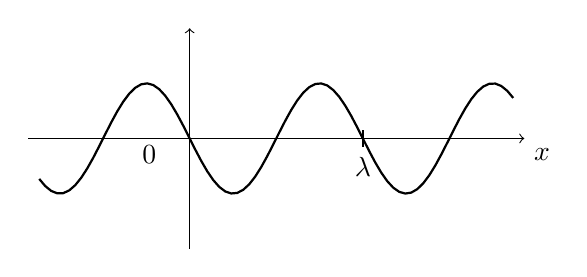
\begin{tikzpicture}[scale=.7]
		\draw[<-] (4.5,0) node[anchor=north west] {$x$}-- (-4.5,0);
		\draw[->] (-pi/2,-2) -- (-pi/2,2); % node[anchor=south east] {$y$};
		\draw[thick,domain=-4.3:4.3, samples=80] plot (\x, {sin(2*\x r)});
		\draw[dotted] (-2,-0.3) node[left] {$0$};
		\draw[thick] (pi/2,0.15) -- (pi/2,-0.15) node[below] {$\lambda$};
	\end{tikzpicture}
\end{minipage}%
\begin{align*}
\Psi_{\pm} (x + n \lambda, t) &= a \cos(k (x + n \lambda) \pm \omega t)\\
&= a \cos( k x \pm \omega t + k n \lambda)\\
&= a \cos(kx \pm \omega t) \\
&= \Psi_{\pm} (x,t)
\end{align*}
Die Kreisfrequenz $ \omega $, Frequenz $ \nu = \frac{\omega}{2 \pi} $, Schwingungsdauer $ \tau = \frac{1}{\nu} = \frac{2 \pi}{\omega} $
\begin{align*}
\Psi_{\pm} (x,t + n \tau) &= a \cos( kx \pm \omega(t + n \tau)) = a \cos(kx \pm \omega t \pm n \ub{\omega \tau}_{= 2 \pi}) \quad n \in \mathbb{Z} \\
&= a \cos(kx \pm \omega t) = \Psi_{\pm}(x,t)
\end{align*}
\begin{center}
	%t4:
	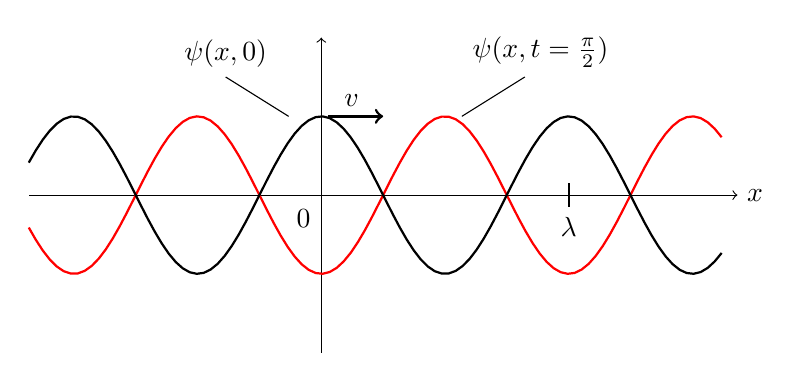
\begin{tikzpicture}
		\draw[<-] (4.5,0) node[right] {$x$}-- (-4.5,0);
		\draw[->] (-pi/4,-2) -- (-pi/4,2); % node[right] {$y$};
		\draw[red,thick,domain=-4.5:4.3, samples=100] plot (\x, {sin(2*\x r)});
		\draw[dotted] (-.8,-0.3) node[left] {$0$};
		\draw[thick] (3*pi/4,0.15) -- ++(0,-0.3) node[below] {$\lambda$};
		\draw[thick,domain=-4.5:4.3, samples=100] plot (\x, {-sin(2*\x r)});
		\draw[dotted] (-0.4,1) node[above] {$v$};
		\draw[dotted] (-2,1.5) node[above] {$\psi(x,0)$};
		\draw (-1.2,1) -- (-2,1.5);
		\draw[line width=1,->] (-0.7,1) -- (0,1);
		\draw[dotted] (2,1.5) node[above] {$\psi(x,t=\frac{\pi}{2})$};
		\draw (1,1) -- (1.8,1.5);
	\end{tikzpicture}
\end{center}
Die Phasengeschwindigkeit $ v $:
\begin{equation*}
v = \frac{\omega}{k} = \frac{\lambda}{2 \pi} \omega = \lambda \nu = \frac{\lambda}{\tau}
\end{equation*}
Ebenso wird die Wellengleichung mit einem Sinus gelöst:
\begin{equation*}
\Psi_{\pm} (x,t) = a \sin(kx \pm \omega t)
\end{equation*}
Beide Lösungen sind also enthalten in:
\begin{equation*}
\Psi(x,t) = a e^{i(\ob{kx - \omega t}^{\varphi \tx{ Phase}})}
\end{equation*}
$ a \in \mathbb{C} \quad k \in \mathbb{R} $\\
$ \omega = v |k| $\\
Für Physikalische Felder gilt:
\begin{equation*}
\Psi(x,t) = \Re\left(a e^{i(kx - \omega t)}\right)
\end{equation*}

\subsection{Ebene Wellen in 3 Raumdimensionen}
\begin{equation*}
\Delta \Psi(\vec{r} ,t) - \frac{1}{v^2} \prt{^2}{t^2} \Psi(\vec{r},t) = 0
\end{equation*}
eben Welle:
\begin{equation*}
\Psi(\vec{r} ,t) = a e^{i (\vec{k} \cdot \vec{r} - \omega t)}
\end{equation*}
Mit dem Wellenvektor:\\
$ \vec{k} = (k_x, k_y, k_z)^\top $\\
und der Frequenz\\
$ \omega \ge 0 $
\begin{align*}
\Delta \Psi &= \left(\prt{^2}{x^2} + \prt{^2}{y^2} + \prt{^2}{z^2}\right) a e^{i(\vec{k} \cdot \vec{r} - \omega t)} \\
&= i^2 (k_x^2 + k_y^2 + k_z^2) a e^{i(\vec{k} \cdot \vec{r} - \omega t)}\\
&= - k^2 \Psi
\end{align*}
\begin{equation*}
\prt{^2 \Psi}{t^2} = - \omega^2 \Psi
\end{equation*}
\begin{equation*}
\Delta \Psi - \frac{1}{v^2} \prt{^2 \Psi}{t^2} = \ob{\left(- k^2 + \frac{\omega^2}{v^2}\right)}^{=0} \Psi = 0
\end{equation*}
$ k^2 = \frac{\omega^2}{v^2} \qquad \omega = v |\vec{k}| $\\[5pt]
\emph{Bemerkung:}\\
\begin{minipage}{.5\linewidth}
	\begin{enumerate}[i)]
		\item ebene Welle:\\
		$ \Psi(\vec{r,t}) $ konstant falls Phase konstant.\\
		$ \varphi (\vec{r} ,t) = \vec{k} \cdot \vec{r} - \omega t = \const $\\
		Für festes $ t $: $ \vec{k} \cdot \vec{r} = \const $
		\item Phasengeschwindigkeit
		\begin{equation*}
		v = \frac{\omega}{|\vec{k}|}
		\end{equation*}
	\end{enumerate}
\end{minipage}%
\begin{minipage}{.5\linewidth}
	\flushright
	%t5:
	\begin{tikzpicture}[scale=.8]
		\draw[->] (0,-1) -- (0,3) node[anchor=south east] {$ y $};
		\draw[->] (-1,0) -- (4.5,0) node[anchor=north west] {$ x $};
		\coordinate (o) at (.5,-1);
		\draw[thick, ->] (o) -- ++(45:4) node[anchor=south west] {$ \vec{x} \  \substack{\tx{Ausbreitungs-} \\ \tx{Richtung}} $ };
		\draw ($ (o) + (135:3) $) -- ++(-45:6);
		\draw ($ (o) + (135:3) + (45:1.5) $) -- ++(-45:6);
		\draw ($ (o) + (135:3) + (45:3) $) -- ++(-45:6);
		\draw[decorate, decoration={brace,amplitude=10pt,raise=18pt}, xshift=2pt, yshift=-2pt]  ($ (o) + (135:2.5) $) -- node[anchor=south east, xshift=-15pt, yshift=15pt] {$\lambda = \frac{2 \pi}{k}$}  ($ (o) + (135:2.5) + (45:1.5) $);
		\draw[thick, <->] ($ (o) + (135:2.5) $) -- ($ (o) + (135:2.5) + (45:1.5) $);
	\end{tikzpicture}
\end{minipage}%
\begin{enumerate}
	\item[iii)] Wellengleichung linear\\
	$ \Rightarrow $ Linearkombinationen von Lösungen sind wieder Lösungen.
	\begin{equation*}
	\Psi(\vec{r},t) = a_1 e^{i(\vec{k}_1 \cdot \vec{r} - \omega_1 t)} + a_2 e^{i(\vec{k}_2 \cdot \vec{r} - \omega_2 t)}
	\end{equation*}
\end{enumerate}
\subsubsection{Allgemeine Lösung der Wellengleichung}
\begin{equation*}
\Psi(\vec{r},t) = \int \dd^3 k \ a(\vec{k}) e^{i(\vec{k} \cdot \vec{r} - \omega t)}
\end{equation*}
\begin{equation*}
\omega(\vec{k}) = v |\vec{k}|
\end{equation*}

\subsection{Ebene elektromagnetische Wellen}

\begin{equation*}
\Rightarrow \quad \rmbox{\Delta \vec{E} - \frac{1}{v^2} \prt{^2 \vec{E}}{t^2} = 0} \qquad 
\Rightarrow \quad \rmbox{\Delta \vec{B} - \frac{1}{v^2} \prt{^2 \vec{B}}{t^2} = 0}
\end{equation*}
Lösungen:
\begin{equation*}
\vec{E} = \vec{E}_0 e^{i(\vec{k} \cdot \vec{r} - \omega t)} \qquad \vec{B} = \vec{B}_0 e^{i(\tilde{\vec{k}} \cdot \vec{r} - \tilde{\omega} t)}
\end{equation*}
$ \omega = v |\vec{k}| \quad \tilde{\omega} = v |\tilde{\vec{k}}| \quad \vec{k}, \tilde{\vec{k}} \in \mathbb{R}^3 $
\begin{enumerate}[i)]
	\item $ \vabla \times \vec{E} = - \prt{\vec{B}}{t} $
	\begin{equation*}
	i (\vec{k} \times \vec{E}_0) e^{i(\vec{k} \cdot \vec{r} - \omega t)} = i \tilde{\omega} \vec{B}_0 e^{i(\tilde{\vec{k}} \cdot \vec{r} - \tilde\omega t)} \qquad \forall \vec{r},t
	\end{equation*}
	$$ \Rightarrow \tilde{\vec{k}} = \vec{k} \quad \tilde{\omega} = \omega $$
	$ \Rightarrow \vec{k} \times \vec{E}_0 = \omega \vec{B}_0 \ \rightarrow \ \vec{B}_0 = \frac{1}{\omega} \vec{k} \times \vec{E}_0 $
	$$\vec{B} \perp \vec{k}, \vec{E}$$
	$$ \Rightarrow \vec{B} = \frac{1}{\omega} \vec{k} \times \vec{E} $$
	\item $ \vabla \cdot \vec{E} = 0 $
	\begin{align*}
	0 &= \vabla \cdot \vec{E}_0 e^{i(\vec{k} \cdot \vec{r} - \omega t)}\\
	&= i(\vec{k} \cdot \vec{E}_0) e^{i(\vec{k} \cdot \vec{r} - \omega t)}
	\end{align*}
	$ \Rightarrow \vec{k} \cdot \vec{E}_0 \ \rightarrow \ \vec{k} \cdot \vec{E}_0 = 0 $
	$$ \vec{k} \perp \vec{E} $$
	\item $ \vabla \cdot \vec{B} = 0 $\\
	$ \Rightarrow \vec{k} \cdot \vec{B}_0 = 0 \Rightarrow \vec{k} \cdot \vec{B} = 0 $\\
	$ \vec{B} \perp \vec{k} $ nichts neues, wissen wir schon aus i)
	\item $ \vabla \times \vec{B} = \frac{1}{v^2} \prt{\vec{E}}{t} $\\
	$ \Rightarrow i \vec{k} \times \vec{B}_0 = - i \frac{1}{v^2} \omega \vec{E}_0 $\\
	$ \Rightarrow \vec{k} \times \vec{B}_0 = - \frac{\omega}{v^2} \vec{E}_0 $\\
	$$ \Rightarrow \vec{E} = -\frac{v^2}{\omega} \vec{k} \times \vec{B} $$
\end{enumerate}
\begin{minipage}{.5\linewidth}
	$ \vec{E}, \vec{B}, \vec{k} $ orthogonal zueinander\\
	$ \Rightarrow $ transversale Welle\\
	Beziehung zwischen der Amplitude von $ \vec{B}, \vec{E} $:
	\begin{equation*}
	|\vec{B}| = \frac{1}{\omega} |\vec{k} \times \vec{E}| = \frac{|\vec{k}|}{\omega} |\vec{E}| = \frac{1}{v} |\vec{E}|
	\end{equation*}
\end{minipage}%
\begin{minipage}{.5\linewidth}
	\flushright
	%t6:
	\begin{tikzpicture}
		\draw[thick,->] (0,0) -- (0,1.5) node[anchor=south east] {$ \vec{E} $};
		\draw[thick,->] (0,0) -- (1.5,0) node[anchor=north west] {$ \vec{S} $};
		\draw[thick,->] (0,0) -- (-.75,-.75) node[anchor=north east] {$ \vec{B} $};
	\end{tikzpicture}
\end{minipage}%
\\
o.B.d.A. $ \quad \vec{k} = k \vec{e}_z $
\begin{align*}
\vec{E} &= (E_{0_x} \vec{e}_x + E_{0_y} \vec{e}_y) e^{i(k \cdot z - \omega t)} \\
\vec{B} &= \frac{1}{\omega} \vec{k} \times \vec{E} = \frac{k}{\omega} \vec{e}_z \times (E_{0_x} \vec{e}_x + E_{0_y} \vec{e}_y) e^{i(k \cdot z - \omega t)} \\
&= \frac{1}{v} (- E_{0_y} \vec{e}_x + E_{0_x} \vec{e}_y) e^{i(k \cdot z - \omega t)} 
\end{align*}
i.A. $ E_{0_x}, E_{0_y} \in \mathbb{C} $
\begin{equation*}
\vec{E} = \Re\left(\vec{E}_0 e^{i(k \cdot z - \omega t)} \right)
\end{equation*}
\emph{Beispiel:} $ E_{0_y} = 0 \quad E_{0_x} \in \mathbb{R} $
\begin{align*}
\vec{E} &= E_{0_x} \cos (kz - \omega t) \vec{e}_x \\
\vec{B} &= \frac{E_{0_x}}{v} \cos(kz - \omega t) \vec{e}_y
\end{align*}

%t7: (EM-Welle Tikz): (v in ausbreitungs richtung einzeichnen)
\begin{center}
	%t3:
	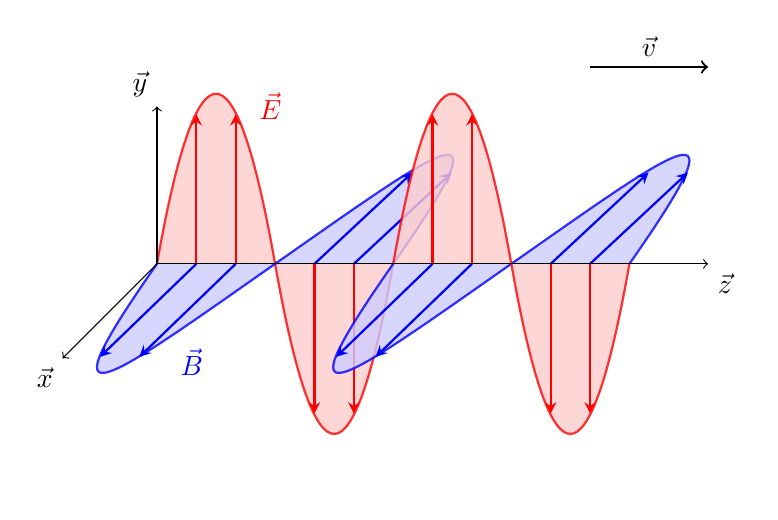
\begin{tikzpicture}%[>=stealth]
	% E
	\draw[red,thick,looseness=5,fill=red!20!white,opacity=.8] (0,0) to[out=80,in=100] (1.5,0) to[out=-80,in=-100] (3,0);
	\foreach \z in {.5,1}
	\draw[thick,red,->,>=stealth] (\z,0) -- ++(0,1.9);
	\foreach \z in {2,2.5}
	\draw[thick,red,->,>=stealth] (\z,0) -- ++(0,-1.9);
	% B
	\draw[blue,thick,looseness=4.5,fill=blue!20!white,opacity=.8] (0,0) to[out=-125,in=-145] (1.5,0) to[out=35,in=55] (3,0) to[out=-125,in=-145] (4.5,0) to[out=35,in=55] (6,0);
	\foreach \z in {.5,1,3.5,4}
	\draw[thick,blue,->,>=stealth] (\z,0) -- ++(-136:1.7cm);
	\foreach \z in {2,2.5,5,5.5}
	\draw[thick,blue,->,>=stealth] (\z,0) -- ++(43:1.7cm);
	% rest E
	\draw[red,thick,looseness=5,fill=red!20!white,opacity=.8] (3,0) to[out=80,in=100] (4.5,0) to[out=-80,in=-100] (6,0);
	\foreach \z in {3.5,4}
	\draw[thick,red,->,>=stealth] (\z,0) -- ++(0,1.9);
	\foreach \z in {5,5.5}
	\draw[thick,red,->,>=stealth] (\z,0) -- ++(0,-1.9);
	% koordinatensystem
	\draw[->] (0,0) -- (0,2) node[anchor=south east] {$ \vec{y} $};
	\draw[->] (0,0) -- (-1.2,-1.2) node[anchor=north east] {$ \vec{x} $};
	\draw[->] (0,0) -- (7,0) node[anchor=north west] {$ \vec{z} $};
	\node (e) at (1.5,2) {\color{red} $ \vec{E} $ \color{black}};
	\node (b) at (.5,-1.25) {\color{blue} $ \vec{B} $ \color{black}};
	\draw[thick,->] (5.5,2.5) -- node[above] {$ \vec{v} $} ++(1.5,0);
	\end{tikzpicture}
\end{center}

\subsection{Polarisation ebener EM-Wellen}

Charakterisierung der Schwingungsrichtung $ \vec{k} = k \vec{e}_z $
\begin{equation*}
\vec{E} = (E_{0_x} \vec{e}_x + E_{0_y} \vec{e}_y) e^{i(kx - \omega t)}
\end{equation*}
\begin{equation*}
E_{0_x} = |E_{0_x}| e^{i \varphi} \qquad E_{0_y} = |E_{0_y}| e^{i (\varphi + \delta)}
\end{equation*}
Physikalisches Feld:
\begin{align*}
\vec{E} &= \Re \left[ (E_{0_x} \vec{e}_x + E_{0_y} \vec{e}_y) e^{i(k \cdot r - \omega t)} \right]\\
&= |E_{0_x}| \cos(kz - \omega t + \varphi) \vec{e}_x + |E_{0_y}| \cos(kz - \omega t + \varphi + \delta) \vec{e}_y
\end{align*}
\textbf{Fälle:}\\
\begin{enumerate}[i)]
	\item
	$ \delta = 0 $ oder $ \delta = \pm \pi $
	\begin{equation*}
	\Rightarrow \quad \vec{E} = \ub{(|E_{0_x}| \vec{e}_x \pm |E_{0_y}| \vec{e}_y)}_{\mathclap{\substack{\tx{orts- und} \\ \tx{Zeitunabh.}}}} \cos(kz - \omega t)
	\end{equation*}
	$ \rightarrow \vec{E} $ schwingt in fester Richtung! Die \textbf{Polarisationsrichtung}
	$ \rightarrow $ \textbf{linear Polarisiert}
	\item
	$ \delta = \pm \frac{\pi}{2} \quad |E_{0_x}| = |E_{0_y}| = E $
	\textbf{Zirkulär Polarisiert}
	\begin{align*}
	\vec{E} = E\ub{(\vec{e}_x \cos(kz - \omega t + \varphi)) \mp \vec{e}_y \sin(kz - \omega t + \varphi))}_{ = \vec{r} (t)}
	\end{align*}
	\lcom{$ |\vec{r}| = 1 $ und $ \vec{r} $ läuft mit $ \omega $ um die $ z $-Achse}
	\item
	$ \delta , |E_{0_x}|, |E_{0_y}| $ beliebig:
	\textbf{elliptisch Polarisiert}
\end{enumerate}
\begin{center}
	%t8:
	\begin{tikzpicture}[scale=.95]
		\draw[->] (0,-2) -- (0,2) node[anchor=south east] {$ y $};
		\draw[->] (-2,0) -- (2,0) node[anchor=north west] {$ x $};
		\draw[thick,->] (0,0) -- (1.2,1.2) node[anchor=south west] {$ \vec{E} $};
		\draw[->] (0,0) -- (-1.2,-1.2);
		\draw[thick] ($ (1.2,0) + (0,.15) $) -- ++(0,-.3) node[below] {$ |E_{0_x}| $};
		\draw[thick] ($ (0,1.2) + (.15,0) $) -- ++(-.3,0) node[left] {$ |E_{0_y}| $};
		%
		\draw[white] (2,-2) -- ++(0,-.225);
	\end{tikzpicture}%
	%t9:
	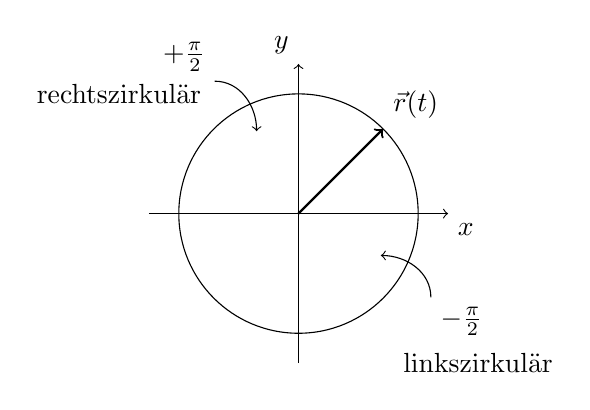
\begin{tikzpicture}[scale=.76]
		\draw[->] (0,-2.5) -- (0,2.5) node[anchor=south east] {$ y $};
		\draw[->] (-2.5,0) -- (2.5,0) node[anchor=north west] {$ x $};
		\draw[thick,->] (0,0) -- ({cos(45) * 2}, {sin(45) * 2}) node[anchor=south west] {$ \vec{r}(t) $};
		\draw (0,0) circle (2cm);
		\centerarc[thick, <->](0,0)(120:-30:1.2);
		\node (a) at (-30:1.4) {};
		\draw[<-] (a) to[out=0,in=90] ++(1,-.7) node[anchor=north west] {$ - \frac{\pi}{2} $};
		\node at (-3,2) {rechtszirkulär};
		\node (b) at (120:1.4) {};
		\draw[<-] (b) to[out=90,in=0] ++(-.7,1) node[anchor=south east] {$ + \frac{\pi}{2} $};
		\node at (3,-2.5) {linkszirkulär};
	\end{tikzpicture}%
	%t10:
	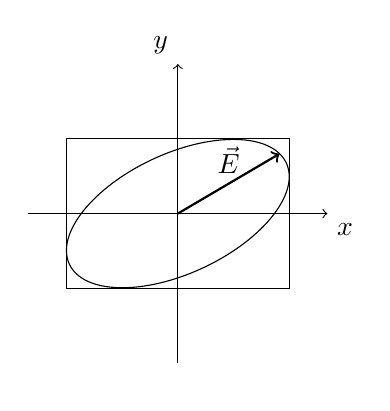
\begin{tikzpicture}[scale=.76]
		\draw[->] (0,-2.5) -- (0,2.5) node[anchor=south east] {$ y $};
		\draw[->] (-2.5,0) -- (2.5,0) node[anchor=north west] {$ x $};
		\draw[rotate=25] (0,0) ellipse (2cm and 1cm);
		\draw (-1.86,-1.25) rectangle (1.86,1.25);
		\draw[thick, ->] (0,0) -- node[above] {$ \vec{E} $} (1.7,1); %({cos(25) * 2},{sin(25) * 2});
		%
		\draw[white] (2,-2.5) -- ++(0,-0.315);
	\end{tikzpicture}
\end{center}

% Vorlesung 10.01.18

\noindent
\bbb{Wiederholung}{
\begin{align*}
\vec{E} &= \vec{E}_0 e^{i(\vec{k} \cdot \vec{r} - \omega t)} \qquad \omega = |\vec{k}| v \\
\vec{B} &= \vec{B}_0 e^{i(\tilde{\vec{k}} \cdot \vec{r} - \tilde{\omega} t)} \ \ \buildrel ! \over = \ \ \frac{1}{\omega} \vec{k} \times \vec{E}
\end{align*}
}

\subsubsection{andere Formen der EM-Wellen}

\begin{minipage}{.45\linewidth}
	\textbf{Wellenpakete:}
	\begin{equation*}
	\vec{E}(\vec{r},t) = \int \dd^3 k \vec{a}(\vec{k}) e^{i(\vec{k} \cdot \vec{r} - \omega(k) t)}
	\end{equation*}
\end{minipage}%
\begin{minipage}{.55\linewidth}
	\flushright
	%t1:
	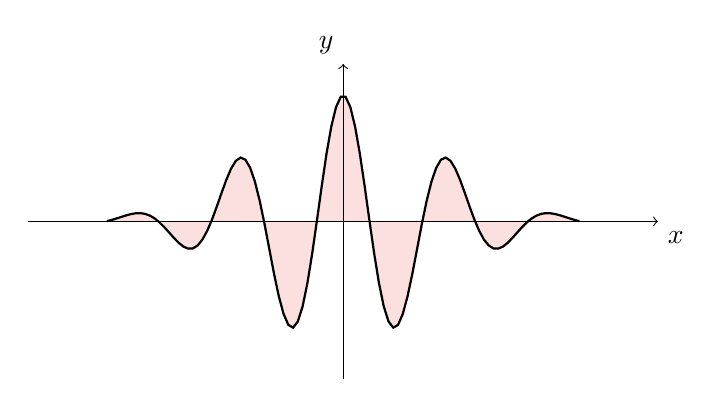
\begin{tikzpicture}[scale=.8]
		\draw[thick,fill=black!10!red!12!white, domain=-3.75:3.75, samples=100] plot (\x, {2 * cos(1 / 4 * 15 * \x r) * exp(- (\x)^(2) * 0.25});
		\draw[->] (-5,0) -- (5,0) node[anchor=north west] {$ x $};
		\draw[->] (0,-2.5) -- (0,2.5) node[anchor=south east] {$ y $};
	\end{tikzpicture}
\end{minipage}%
\\
\begin{minipage}{.5\linewidth}
	\textbf{Kugelwellen}
	\begin{equation*}
	\vec{E}(\vec{r},t) = \vec{E}_0 \frac{e^{i(\vec{k} \cdot \vec{r} - \omega t)}}{r}
	\end{equation*}
	eine Kugelwelle hat Amplitude $ \rho \propto \frac{1}{r} $\\
	Flächen gleicher Phase (wie im Bild zu sehen).
	\begin{center}
		%t2:
		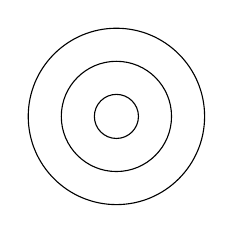
\begin{tikzpicture}[scale=.7]
			\draw (0,0) circle (.4cm);
			\draw (0,0) circle (1cm);
			\draw (0,0) circle (1.6cm);
		\end{tikzpicture}
	\end{center}
\end{minipage}%
\begin{minipage}{.5\linewidth}
	\flushright
	%t3:
	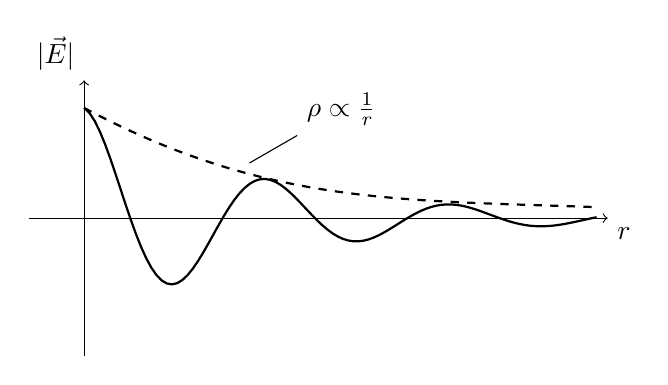
\begin{tikzpicture}[scale=.7]
		\draw[->] (-1,0) -- (9.5,0) node[anchor=north west] {$ r $};
		\draw[->] (0,-2.5) -- (0,2.5) node[anchor=south east] {$ |\vec{E}| $};
		\draw[thick,domain=0.001:9.3, samples=100] plot (\x, {2 * cos(1 / 4 * 15 * (\x * .5) r) * exp(- (\x * .5)^(2) * 0.25 * (1) / (\x * 0.2) });
		\draw[thick, dashed] (0,2) to[out=-28,in=178] (9.3,.2);
		\draw (3,1) -- ++(30:1cm) node[anchor=south west] {$ \rho \propto \frac{1}{r} $};
	\end{tikzpicture}
\end{minipage}%

\section{Reflexion und Brechung von EM-Wellen an Grenzflächen}

Wir betrachten eine ebene Grenzfläche ($ x $-$ y $-Ebene) zwischen zwei ungeladenen, nicht leitenden Medien.\\
\begin{minipage}{.55\linewidth}
	Aus der Skizze:
	\begin{equation*}
	v_1 = \frac{1}{\sqrt{\epsilon_1 \mu_1}} , \ \omega_e = v_1 k_e
	\end{equation*}
	und $ \vec{k}_e $ ohne $ y $-Komponente
	\begin{equation*}
	\vec{k}_e = \begin{pmatrix}
	k_{e_x} \\ 0 \\ k_{e_z}
	\end{pmatrix}
	\end{equation*}
\end{minipage}%
\begin{minipage}{.45\linewidth}
	%t4:
	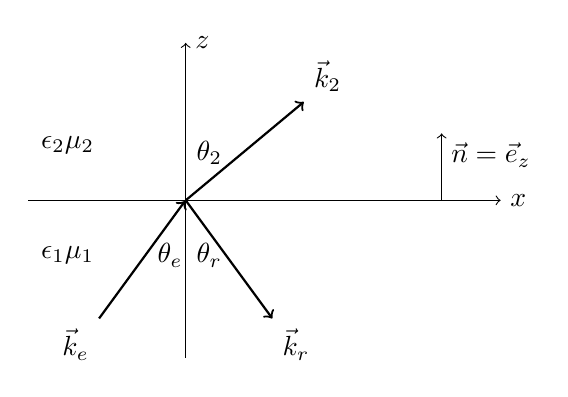
\begin{tikzpicture}
		\draw[->] (-2,0) -- (4,0) node[right] {$x$};
		\draw[->] (0,-2) -- (0,2) node[right] {$z$};
		\draw[thick,->] (-1.1,-1.5) node[anchor=north east] {$\vec{k}_e$} -- (-0.01,-0.01); 
		\draw[thick,->] (0,0) -- (1.5,1.25) node[anchor=south west] {$\vec{k}_2$}; 
		\draw[thick,->] (0,0) -- (1.1,-1.5) node[anchor=north west] {$\vec{k}_r$};
		\centerarc[](0,0)(40:90:1);
		\node at (0.3,0.6) {$\theta_2$};
		\centerarc[](0,0)(234:270:1);
		\node at (-0.2,-0.7) {$\theta_e$};
		\centerarc[](0,0)(270:306:1);
		\node at (0.3,-0.7) {$\theta_r$};
		\node at (-1.5,.7) {$\epsilon_2 \mu_2$};
		\node at (-1.5,-.7) {$\epsilon_1 \mu_1$};
		\draw[->] (3.25,0) -- (3.25,.85) node[anchor=north west] {$\vec{n}=\vec{e}_z$};
	\end{tikzpicture}
	\vspace{5pt}
\end{minipage}%
\\
Die \textbf{einfallende Welle} sieht folgendermaßen aus:
\begin{align*}
\vec{E}_e &= \vec{E}_{e_0} e^{i(\vec{k}_e \cdot \vec{r} - \omega_e t)}\\
\vec{B}_e &= \frac{1}{\omega_e} \vec{k}_e \times \vec{E}_e = \frac{1}{v_1} \frac{\vec{k}_e}{k_e} \times \vec{E}_e
\end{align*}
\textbf{reflektierte Welle}
\begin{align*}
\vec{E}_r &= \vec{E}_{r_0} e^{i(\vec{k}_r \cdot \vec{r} - \omega_r t)} \\
\vec{B}_r &= \frac{1}{v_1} \frac{\vec{k}_r}{k_r} \times \vec{E}_r
\end{align*}
gesamtes Feld in Medium 1:
\begin{equation*}
\vec{E}_1 = \vec{E}_e + \vec{E}_r
\end{equation*}
\textbf{transmittierte Welle}
\begin{align*}
\vec{E}_2 &= \vec{E}_{2_0} e^{i(\vec{k}_2 \cdot \vec{r} - \omega_2 t)} \\
\vec{B}_2 &= \frac{1}{v_2} \frac{\vec{k}_2}{k_2} \times \vec{E}_2
\end{align*}

\subsection{Stetigkeitsbedingunen an Grenzflächen}

Hier: ungeladene, nicht leitende Medien: $ \rho_f = 0 = \vec{j}_f $\\[5pt]
Maxwell-Gl. $ \Rightarrow $ Stetigkeitsbedingungen für $ \vec{r} = (x,y,0) $
\begin{enumerate}[i)]
	\item mit $ \vabla \cdot \vec{D} = 0 $
	\begin{equation*}
	\vec{n} \cdot (\vec{D}_1 - \vec{D}_2) = 0 \quad \Rightarrow \quad \epsilon_1 \vec{n} \cdot \vec{E}_1 - \epsilon_2 \vec{n} \cdot \vec{E}_2 = 0
	\end{equation*}
	\item mit $ \vabla \times \vec{E} = - \prt{\vec{B}}{t} $ und $ \vec{t} \sim \vec{e}_x, \vec{e}_y $
	\begin{equation*}
	\vec{t} \cdot (\vec{E}_1 - \vec{E}_2) = 0
	\end{equation*}
	\item mit $ \vabla \cdot \vec{B} = 0 $
	\begin{equation*}
	\vec{n} \cdot (\vec{B}_1 - \vec{B}_2) = 0
	\end{equation*}
	\item mit $ \vabla \times \vec{H} = \cancel{\vec{j}} + \prt{\vec{D}}{t} $
	\begin{equation*}
	\vec{t} \cdot (\vec{H}_1 - \vec{H}_2) = 0 \quad \Rightarrow \quad \frac{1}{\mu_1} \vec{t} \cdot \vec{B}_1 - \frac{1}{\mu_2} \vec{t} \cdot \vec{B}_2 = 0
	\end{equation*}
\end{enumerate}
Erläuterung zu Punkt ii) und iv):
\begin{equation*}
\vabla \times \vec{E} = - \prt{\vec{B}}{t} \quad \rightarrow \quad \vec{t} \cdot (\vec{E}_2 - \vec{E}_1) = 0
\end{equation*}
\begin{minipage}{.6\linewidth}
	\begin{align*}
	&\int \limits _F \dd \vec{f} \cdot (\vabla \times \vec{E}) = - \int \limits_F \dd \vec{f} \cdot \prt{\vec{B}}{t} = \ub{- \prd{}{t} \int \limits_F \dd \vec{f} \vec{B}}_{\overset{\Delta x \to 0}{\rightarrow} 0} \\
	= & \int \limits_{\partial F} \dd \vec{r} \cdot \vec{E} \qquad \rightarrow \qquad \int \dd s \ \vec{t} \cdot (\vec{E}_2 - \vec{E}_1) = 0
	\end{align*}
	\vspace{5pt}
\end{minipage}%
\begin{minipage}{.4\linewidth}
	\flushright
	%t5:
	\begin{tikzpicture}[scale=.7]
		\draw[->] (-2.2,0) -- (3,0) node[anchor=north west] {$ y $};
		\draw[->] (0,-2) -- (0,2) node[anchor=south east] {$ x $};
		\draw[thick] (-2,-1) rectangle (2,1);
		\draw[ultra thick, ->] (0,0) -- (1,0);
		\draw (.5,-.2) -- ++(-60:1.5cm) node[below=2pt] {$ \vec{E} $};
		\draw[decorate, decoration={brace,amplitude=10pt,raise=2pt}, thick]  ($ (-2,-1) $) -- node[left, xshift=-15pt] {$\Delta x$}  ($ (-2,1) $);
	\end{tikzpicture}
\end{minipage}%
\\
Aus den vier Stetigkeitsbedingungen ergeben sich folgende Schlussfolgerungen:\\[5pt]
ii)
\begin{equation*}
\vec{t} \cdot \vec{E}_2 = \vec{t} \cdot \vec{E}_1 = \vec{t} \cdot (\vec{E}_e + \vec{E}_r)
\end{equation*}
\begin{equation*}
\Rightarrow \vec{t} \cdot \vec{E}_{2_0}  e^{i(\vec{k}_2 \cdot \vec{r} - \omega_2 t)} = \vec{t} \cdot \vec{E}_{e_0}  e^{i(\vec{k}_e \cdot \vec{r} - \omega_e t)} + \vec{t} \cdot \vec{E}_{r_0}  e^{i(\vec{k}_r \cdot \vec{r} - \omega_r t)}
\end{equation*}
$ \forall \vec{r} = (x,y,0) , \forall t $
$ \rightarrow $ Die Orts- und Zeitabhängigkeit im Exponenten muss gleich sein!
\begin{equation*}
\vec{k}_2 \cdot \vec{r} - \omega_2 t =  \vec{k}_e \cdot \vec{r} - \omega_e t = \vec{k}_r \cdot \vec{r} - \omega_r t
\end{equation*}
$ \vec{r} = 0 : $ $ \Rightarrow \ \omega_2 = \omega_e = \omega_r \defeq \omega $\\
\lcom{Die gleiche Schlussfolgerung geht für die Wellenvektoren nicht, da wir hier die $ z $-Kompo-\\
nente gar nicht beachten und damit keine Aussagen über die Gleichheit der Vektoren machen können.}\\[5pt]
Für die einfallende und reflektierte Welle im Medium 1 gilt:\\
$ v_1 = \frac{\omega_e}{|\vec{k}_e|} = \frac{\omega_r}{|\vec{k}_r|} $
\begin{equation*}
\rightarrow \quad |\vec{k}_e| = |\vec{k}_r| \defeq k_1
\end{equation*}
Somit sind auch beide Wellenlängen $ \lambda_1 $ gleich!\\[5pt]
Für die Welle im Medium 2 gilt:
\begin{align*}
k_2 &= \frac{\omega_2}{v_2} = \omega \sqrt{\epsilon_2 \mu_2} \\
&= \omega \sqrt{\frac{\epsilon_2 \mu_2}{\epsilon_1 \mu_1}} \sqrt{\epsilon_1 \mu_1} = \ub{\frac{\omega}{v_1}}_{k_1} \sqrt{\frac{\epsilon_2 \mu_2}{\epsilon_1 \mu_1}} = 	k_1 \sqrt{\frac{\epsilon_2 \mu_2}{\epsilon_1 \mu_1}} = k_1 \cdot \frac{n_2}{n_1}
\end{align*}
weiterhin:
$ t=0 : $ $ \Rightarrow \ \vec{k}_2 \cdot \vec{r} = \vec{k}_e \cdot \vec{r} = \vec{k}_r \cdot \vec{r} $\\[5pt]
$ k_{2_x} x + k_{2_y} y = k_{e_x} x + \ub{k_{e_y} y}_{=0} = k_{r_x} x + k_{r_y} y =   $\\[5pt]
$ k_{e_y} = 0 \quad \Rightarrow k_{2_y} = 0 = k_{r_y}$
$ \Rightarrow \vec{k}_e, \vec{k}_r, \vec{k}_2 $ liegen in einer Ebene (hier: $ x $-$ z $-Ebene), der Einfallsebene.\\
\begin{minipage}{.5\linewidth}
	\begin{align*}
	\vec{k}_e &= k_e (\sin \theta_e \vec{e}_x + \cos \theta _e \vec{e}_z)\\
	\vec{k}_r &= k_r (\sin \theta_r \vec{e}_x - \cos \theta _r \vec{e}_z)\\
	\vec{k}_2 &= k_2 (\sin \theta_2 \vec{e}_x + \cos \theta _2 \vec{e}_z)
	\end{align*}
	$ k_e = k_r \defeq k_1 $
\end{minipage}%
\begin{minipage}{.5\linewidth}
	\flushright
	%t6:
	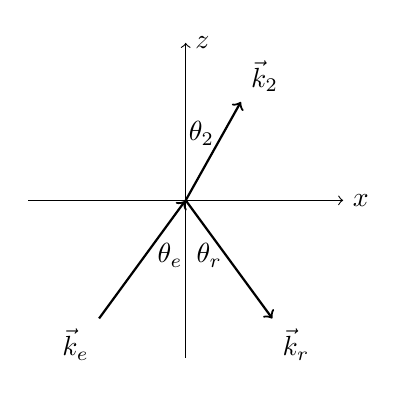
\begin{tikzpicture}
		\draw[->] (-2,0) -- (2,0) node[right] {$x$};
		\draw[->] (0,-2) -- (0,2) node[right] {$z$}; 
		\draw[thick,->] (0,0) -- (0.7,1.25) node[anchor=south west] {$\vec{k}_2$}; 
		\centerarc[](0,0)(60:90:1.2);
		\node at (0.2,.85) {$\theta_2$};
		\draw[thick,->] (-1.1,-1.5) node[anchor=north east] {$\vec{k}_e$} -- (-0.01,-0.01); 
		\draw[thick,->] (0,0) -- (1.1,-1.5) node[anchor=north west] {$\vec{k}_r$};
		\centerarc[](0,0)(234:270:1);
		\node at (-0.2,-0.7) {$\theta_e$};
		\centerarc[](0,0)(270:306:1);
		\node at (0.3,-0.7) {$\theta_r$};
	\end{tikzpicture}
\end{minipage}%

\subsubsection{Reflexionsgesetz}

$ \vec{r} = (x,0,0): \quad \vec{k}_e \cdot \vec{r} = \vec{k}_r \cdot \vec{r} $
\begin{align*}
\vec{k}_e \cdot \vec{r} &= x k_1 \sin \theta_e\\
\vec{k}_r \cdot \vec{r} &= x k_1 \sin \theta_r\\
\end{align*}
\begin{center}
	\begin{minipage}{.5\linewidth}
		\frbox{Reflexionsgesetz}{
		\begin{equation*}
		\theta_e = \theta_r
		\end{equation*}
		}
	\end{minipage}
\end{center}


\subsubsection{Brechungsgesetz}

$ \vec{r} = (x,0,0): \quad \vec{k}_2 \cdot \vec{r} = \vec{k}_e \cdot \vec{r} $
\begin{align*}
&k_2 \sin \theta_2 = k_1 \sin \theta_1 \\
k_2 = &k_1 \sqrt{\frac{\epsilon_2 \mu_2}{\epsilon_1 \mu_1}} = k_1 \frac{n_2}{n_1}
\end{align*}
$ n : $ Brechungsindex
\begin{center}
	\begin{minipage}{.5\linewidth}
		\frbox{Snellius'sches Brechungsgesetz}{
		\begin{equation*}
		\frac{n_2}{n_1} = \frac{\sin \theta_1}{\sin \theta_2}
		\end{equation*}
		}
	\end{minipage}
\end{center}
\begin{center}
	%t7:
	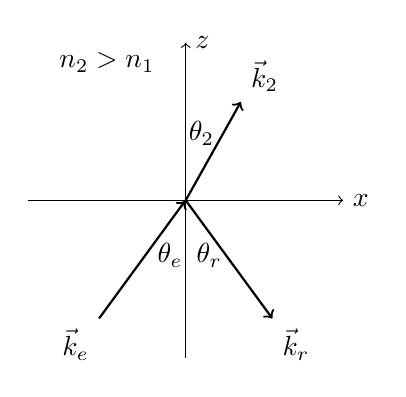
\begin{tikzpicture}
		\draw[->] (-2,0) -- (2,0) node[right] {$x$};
		\draw[->] (0,-2) -- (0,2) node[right] {$z$};
		\draw[thick,->] (0,0) -- (0.7,1.25) node[anchor=south west] {$\vec{k}_2$}; 
		\centerarc[](0,0)(60:90:1.2);
		\node at (0.2,.85) {$\theta_2$};
		\draw[thick,->] (-1.1,-1.5) node[anchor=north east] {$\vec{k}_e$} -- (-0.01,-0.01);
		\draw[thick,->] (0,0) -- (1.1,-1.5) node[anchor=north west] {$\vec{k}_r$};
		\centerarc[](0,0)(234:270:1);
		\node at (-0.2,-0.7) {$\theta_e$};
		\centerarc[](0,0)(270:306:1);
		\node at (0.3,-0.7) {$\theta_r$};
		\node at (-1,1.75) {$n_2>n_1$};
	\end{tikzpicture}
	\hspace{1.5cm}
	%t8:
	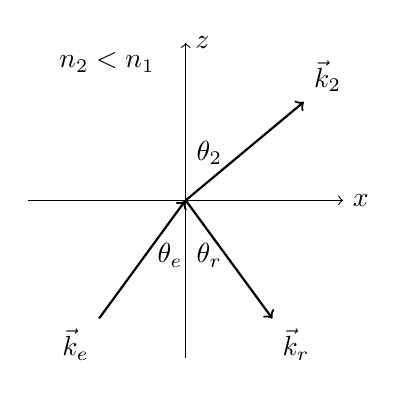
\begin{tikzpicture}
		\draw[->] (-2,0) -- (2,0) node[right] {$x$};
		\draw[->] (0,-2) -- (0,2) node[right] {$z$}; 
		\draw[thick,->] (0,0) -- (1.5,1.25) node[anchor=south west] {$\vec{k}_2$}; 
		\centerarc[](0,0)(40:90:1);
		\node at (0.3,0.6) {$\theta_2$};
		\draw[thick,->] (-1.1,-1.5) node[anchor=north east] {$\vec{k}_e$} -- (-0.01,-0.01); 
		\draw[thick,->] (0,0) -- (1.1,-1.5) node[anchor=north west] {$\vec{k}_r$};
		\centerarc[](0,0)(234:270:1);
		\node at (-0.2,-0.7) {$\theta_e$};
		\centerarc[](0,0)(270:306:1);
		\node at (0.3,-0.7) {$\theta_r$};
		\node at (-1,1.75) {$n_2<n_1$};
	\end{tikzpicture}
\end{center}
Für $ n_2 > n_1 : $ Grenzfall $ \theta_1 \defeq \theta_g $ bei dem \textbf{Totalreflexion} auftritt (d.h. $ \theta_2 = \frac{\pi}{2} $)
\begin{equation*}
\sin \theta_g = \frac{n_2}{n_1} \sin \frac{\pi}{2} = \frac{n_2}{n_1}
\end{equation*}
z.B. Wasser $ \ n_1 \approx 1{,}33 $, Luft $ \ n_2 \approx 1 $ $ \Rightarrow \theta_g \approx 49 ^\circ $
\begin{comment}
\begin{tikzpicture}
\draw[->] (-5,0) -- (5,0);
\draw[->] (0,-5) -- (0,5);
\draw [domain=-3.75:3.75, samples=100] plot (\x, {2 * cos(1 / 4 * 15 * \x r) * exp(- (\x)^(2) * 0.25});
\end{tikzpicture}
\end{comment}
% teyt of tikz plotting:
%\begin{tikzpicture}
%\draw [domain=-4:4, samples=100,scale=.3] plot (\x, {5*exp(-(\x)^(2)*0.25 * cos(\x * 40)});
%\end{tikzpicture}

%Vorlesung 14.01.18

\subsection{Intensitätsbeziehungen bei Reflexion und Brechung}

\bbb{Wiederholung}{
\begin{minipage}{.6\linewidth}
	\begin{equation*}
	\vec{E}_l = \vec{E}_{l_0} e^{i(\vec{k}_l \vec{r} - \omega t)} \qquad l = e, r, 2
	\end{equation*}
	\begin{align*}
	\vec{B}_l &= \frac{1}{\omega} \vec{k}_e \times \vec{E}_l \\
	\vec{E}_1 &= \vec{E}_e + \vec{E}_r
	\end{align*}
\end{minipage}%
\begin{minipage}{.4\linewidth}
	%t1:
	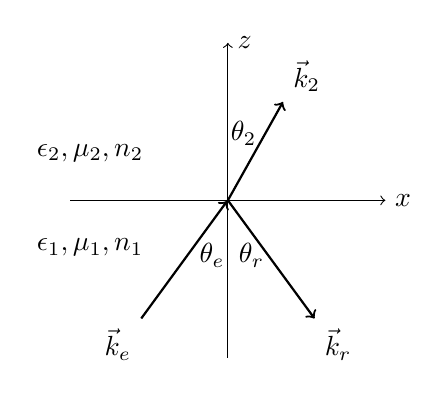
\begin{tikzpicture}
		\draw[->] (-2,0) -- (2,0) node[right] {$x$};
		\draw[->] (0,-2) -- (0,2) node[right] {$z$};
		\draw[thick,->] (0,0) -- (0.7,1.25) node[anchor=south west] {$\vec{k}_2$}; 
		\centerarc[](0,0)(60:90:1.2);
		\node at (0.2,.85) {$\theta_2$};
		\draw[thick,->] (-1.1,-1.5) node[anchor=north east] {$\vec{k}_e$} -- (-0.01,-0.01);
		\draw[thick,->] (0,0) -- (1.1,-1.5) node[anchor=north west] {$\vec{k}_r$};
		\centerarc[](0,0)(234:270:1);
		\node at (-0.2,-0.7) {$\theta_e$};
		\centerarc[](0,0)(270:306:1);
		\node at (0.3,-0.7) {$\theta_r$};
		\node at (-1.75,.6) {$ \epsilon_2, \mu_2, n_2 $};
		\node at (-1.75,-.6) {$ \epsilon_1, \mu_1, n_1 $};
	\end{tikzpicture}
	\vspace{5pt}
\end{minipage}%
\\
\textbf{Stetigkeitsbedingungen an der Grenzfläche} $ \vec{r} = (x,y,0) $ hier: $ \vec{r} = 0  , \ t = 0 \quad \vec{t} \sim \vec{e}_x , \vec{e}_y $
\begin{enumerate}[i)]
	\item
	\begin{equation*}
	\vec{n} \cdot (\vec{D}_2 - \vec{D}_1) = 0
	\end{equation*}
	\begin{equation*}
	\Rightarrow \quad \vec{e}_z \cdot (\epsilon_2 \vec{E}_{2_0} - \epsilon_1 (\vec{E}_{e_0} + \vec{E}_{r_0})) = 0
	\end{equation*}
	\item
	\begin{equation*}
	\vec{t} \cdot (\vec{E}_2 - \vec{E}_1) = 0
	\end{equation*}
	\begin{equation*}
	\Rightarrow \quad \vec{t} \cdot (\vec{E}_{2_0} - \vec{E}_{e_0} - \vec{E}_{r_0}) = 0
	\end{equation*}
	\item
	\begin{equation*}
	\vec{n} \cdot (\vec{B}_2 - \vec{B}_1) = 0
	\end{equation*}
	\begin{equation*}
	\Rightarrow \quad \vec{e}_z \cdot \bigg[\vec{k}_2 \times \vec{E}_{2_0} - \vec{k}_e \times \vec{E}_{e_0} - \vec{k}_r \times \vec{E}_{r_0}\bigg] = 0
	\end{equation*}
	\item
	\begin{equation*}
	\vec{t} \cdot (\vec{H}_2 - \vec{H}_1) = 0 \qquad \vec{H}_i = \frac{1}{\mu} \vec{B}_i
	\end{equation*}
	\begin{equation*}
	\Rightarrow \quad \vec{t} \cdot \bigg[\frac{1}{\mu_2} \vec{k}_2 \times \vec{E}_{2_0} - \frac{1}{\mu_1} \vec{k}_r \times \vec{E}_{r_0} - \frac{1}{\mu_1} \vec{k}_e\ \times \vec{E}_{e_0} \bigg] = 0
	\end{equation*}
\end{enumerate}
}

\noindent
Wir zerlegen die Amplitude der einfallenden Welle in Anteile parallel und senkrecht zur Einfallsebene ($ x $-$ z $-Ebene).
\begin{align*}
\vec{E}_{e_0} &= \vec{E}_{e_{0_\parallel}} + \vec{E}_{e_{0_\perp}} \\
\vec{E}_{e_{0_\perp}} &= (\vec{e}_y \cdot \vec{E}_{e_0}) \cdot \vec{e}_y
\end{align*}
$ \Rightarrow \quad \vec{E}_e = \vec{E}_{e_\parallel} + \vec{E}_{e_\perp} $\\
ebenso für $ \vec{E}_r $ und $ \vec{E}_2 $\\[10pt]
\lcom{Den einen Fall betrachten wir genauer die anderen sind ähnlich und werden deswegen nicht genauer besprochen.}
\begin{enumerate}[I)]
	\item $ \vec{E}_e $ senkrecht zur Einfallsebene polarisiert:
	$$ \vec{E}_{e_0}  = E_{e_0} \vec{e}_y $$
	\begin{minipage}{.6\linewidth}
		Es folgt aus der Skizze:
		\begin{align*}
		\vec{k}_2 &= k_2 (\sin \theta_2 \vec{e}_x + \cos \theta_2 \vec{e}_z)\\
		\vec{k}_e &= k_e (\sin \theta_1 \vec{e}_x + \cos \theta_1 \vec{e}_z)\\
		\vec{k}_r &= k_r (\sin \theta_1 \vec{e}_x + \cos \theta_1 \vec{e}_z)
		\end{align*}
	\end{minipage}%
	\begin{minipage}{.4\linewidth}
		\flushright
		%t2:
		\begin{tikzpicture}
			\draw[->] (-2.5,0) -- (2.5,0) node[right] {$x$};
			\draw[->] (0,-2.5) -- (0,2.5) node[right] {$z$};
			\draw[thick,->] (0,0) -- (30:2.5cm) node[anchor=south west] {$\vec{k}_2$}; 
			\centerarc[](0,0)(30:90:.9);
			\node at (0.3,.5) {$\theta_2$};
			\draw[thick,->] (-135:2.5cm) node[anchor=north east] {$\vec{k}_e$} -- (-0.01,-0.01);
			\node at (-0.2,-0.5) {$\theta_e$};
			\centerarc[](0,0)(-90:-45:.9);
			\draw[thick,->] (0,0) -- (-45:2.5cm) node[anchor=north west] {$\vec{k}_r$};
			\centerarc[](0,0)(-135:-90:.9);
			\node at (0.25,-0.5) {$\theta_r$};
			%E und B Felder
			\coordinate (2) at (30:1.5);
			\draw[black!20!blue,thick,->] (2) -- node[anchor=south west] {$ \vec{B}_2 $} ++(120:1cm);
			\draw[black!15!red,thick] (2) circle (.15cm);
			\draw[black!15!red,thick] ($ (2) + (-135+30:.15) $) -- ++(45+30:.3);
			\draw[black!15!red,thick] ($ (2) + (135+30:.15) $) -- ++(-45+30:.3);
			\node[black!15!red,anchor=north west] at (2) {$ \vec{E}_2 $};
			%
			\coordinate (e) at (-135:1.5);
			\draw[black!20!blue,thick,->] (e) -- node[anchor=north east] {$ \vec{B}_e $} ++(135:1cm);
			\draw[black!15!red,thick] (e) circle (.15cm);
			\draw[black!15!red,thick] ($ (e) + (-135+45:.15) $) -- ++(45+45:.3);
			\draw[black!15!red,thick] ($ (e) + (135+45:.15) $) -- ++(-45+45:.3);
			\node[black!15!red,anchor=north west] at (e) {$ \vec{E}_e $};
			%
			\coordinate (r) at (-45:1.5);
			\draw[black!20!blue,thick,->] (r) -- node[anchor=north west] {$ \vec{B}_r $} ++(45:1cm);
			\draw[black!15!red,thick] (r) circle (.15cm);
			\draw[black!15!red,thick] ($ (r) + (-135+45:.15) $) -- ++(45+45:.3);
			\draw[black!15!red,thick] ($ (r) + (135+45:.15) $) -- ++(-45+45:.3);
			\node[black!15!red,anchor=north east] at (r) {$ \vec{E}_r $};
		\end{tikzpicture}
	\end{minipage}%
	\\
	Aus den Stetigkeitsbedingunen folgt:  % vielleicht muss eins auch i) sein
	\begin{equation*}
	\vec{E}_{r_0} = E_{r_0} \vec{e}_y \qquad \vec{E}_{2_0} = E_{2_0} \vec{e}_y
	\end{equation*}
	\begin{enumerate}
		\item[ii)] $ \vec{t} = \vec{e}_y $
		\begin{equation*}
		\Rightarrow \quad \rmbox{0 = E_{2_0} - E_{e_0} - E_{r_0}}
		\end{equation*}
		\item[iii)] Diese Bedingung liefert im wesentlichen das Brechungsgesetz
		\item[iv)] $ \vec{t} = \vec{e}_x: $
		%
		%
		%
		% make me nicer:
		%
		%
		%
		\begin{equation*}
		0 = \frac{1}{\mu_2} \ub{\vec{e}_x \cdot (\vec{k}_2 \times \vec{E}_{2_0})}_{\substack{= - \vec{k}_2 \cdot (\vec{e}_x \times \vec{E}_{2_0}) \\ = - \vec{k}_2 \cdot \vec{e}_z E_{2_0} \\ = - E_{2_0} k_2 \cos \theta_2}} - \frac{1}{\mu_1} \ub{\vec{e}_x \cdot (\vec{k}_e \times \vec{E}_{e_0})}_{= - E_{e_0} k_e \cos \theta_1} - \frac{1}{\mu_1} \ub{\vec{e}_x \cdot (\vec{k}_r \times \vec{E}_{r_0})}_{= E_{r_0} k_r \cos \theta_1}
		\end{equation*}
		\begin{equation*}
		\Rightarrow \quad \rmbox{0 = - \frac{k_2}{\mu_2} E_{2_0} \cos \theta_2 + \frac{k_e}{\mu_1} E_{e_0} \cos \theta_1 - \frac{k_r}{\mu_1} E_{r_0} \cos \theta_1}
		\end{equation*}
	\end{enumerate}
	$ E_{r_0} = E_{2_0} - E_{e_0} $\\[5pt]
	$ k_e = k_r = k_1 = \frac{\omega}{v_1} = \omega \sqrt{\epsilon_1 \mu_1} $\\
	$ k_2 = \omega \sqrt{\epsilon_2 \mu_2} $
	\begin{equation*}
	\Rightarrow \quad 0 = - \omega \sqrt{\frac{\epsilon_2}{\mu_2}} E_{2_0} \cos \theta_2 + \omega \sqrt{\frac{\epsilon_1}{\mu_1}} E_{e_0} \cos \theta_1 - \omega \sqrt{\frac{\epsilon_1}{\mu_1}} (E_{2_0} - E_{e_0}) \cos \theta_1
	\end{equation*}
	Umformen mit Brechungsindex $ n_i = \sqrt{\epsilon_{r_i} \mu_{e_i}} $
	\begin{equation*}
	\Rightarrow \quad \left(\frac{E_{2_0}}{E_{e_0}}\right)_{\perp} = \frac{2\sqrt{\frac{\epsilon_1}{\mu_1}} \cos \theta_1}{\sqrt{\frac{\epsilon_1}{\mu_1}} \cos \theta_1 + \sqrt{\frac{\epsilon_2}{\mu_2}} \cos \theta_2} = \frac{2 n_1 \cos \theta_1}{n_1 \cos \theta_1 + \frac{\mu_1}{\mu_2} n_2 \cos \theta_2}
	\end{equation*}
	Einfalls- und Ausfallswinkel können wir mit dem Brechungsgesetz ineinander umformen: $ \cos \theta_2 = \sqrt{1 - \sin^2 \theta_2} = \sqrt{1 - \frac{n_1^2}{n_2^2} \sin^2 \theta_1} $ und
	$ E_{r_0} = E_{2_0} - E_{e_0} $\\[5pt]
	\frbox{Senkrechter Einfall}{
	\begin{equation*}
	\Rightarrow \quad \left(\frac{E_{2_0}}{E_{e_0}}\right)_{\perp} = \frac{n_1 \cos \theta_1 - \frac{\mu_1}{\mu_2} n_2 \cos \theta_2}{n_1 \cos \theta_1 + \frac{\mu_1}{\mu_2} n_2 \cos \theta_2}
	\end{equation*}
	}
	%
	%
	%
	\pagebreak
	%
	%
	%
	\item  $ \vec{E}_e $ parallel zur Einfallsebene\\
	\frbox{Paralleler Einfall}{
	\begin{equation*}
	\left(\frac{E_{2_0}}{E_{e_0}}\right)_{\parallel} = \frac{2 n_1 \cos \theta_1}{\frac{\mu_1}{\mu_2}n_2 \cos \theta_1 + n_1 \cos \theta_2}
	\end{equation*}
	\begin{equation*}
	\left(\frac{E_{r_0}}{E_{e_0}}\right)_{\parallel} = \frac{\frac{\mu_1}{\mu_2} n_2 \cos \theta_1 - n_1 \cos \theta_2}{\frac{\mu_1}{\mu_2} n_2 \cos \theta_1 + n_1 \cos \theta_2}
	\end{equation*}
	}
	\begin{center}
		%t3:
		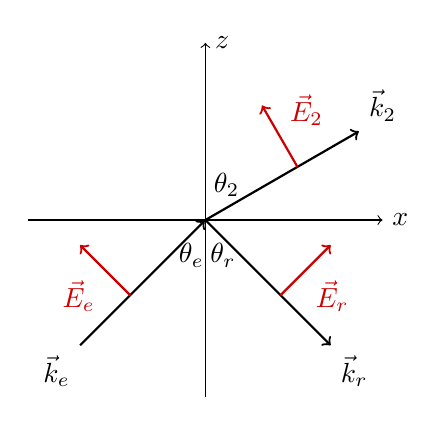
\begin{tikzpicture}[scale=.9]
		\draw[->] (-2.5,0) -- (2.5,0) node[right] {$x$};
		\draw[->] (0,-2.5) -- (0,2.5) node[right] {$z$};
		\draw[thick,->] (0,0) -- (30:2.5cm) node[anchor=south west] {$\vec{k}_2$}; 
		\centerarc[](0,0)(30:90:.9);
		\node at (0.3,.5) {$\theta_2$};
		\draw[thick,->] (-135:2.5cm) node[anchor=north east] {$\vec{k}_e$} -- (-0.01,-0.01);
		\node at (-0.2,-0.5) {$\theta_e$};
		\centerarc[](0,0)(-90:-45:.9);
		\draw[thick,->] (0,0) -- (-45:2.5cm) node[anchor=north west] {$\vec{k}_r$};
		\centerarc[](0,0)(-135:-90:.9);
		\node at (0.25,-0.5) {$\theta_r$};
		%E und B Felder
		\coordinate (2) at (30:1.5);
		\draw[black!20!red,thick,->] (2) -- node[anchor=south west] {$ \vec{E}_2 $} ++(120:1cm);
		%
		\coordinate (e) at (-135:1.5);
		\draw[black!20!red,thick,->] (e) -- node[anchor=north east] {$ \vec{E}_e $} ++(135:1cm);
		%
		\coordinate (r) at (-45:1.5);
		\draw[black!20!red,thick,->] (r) -- node[anchor=north west] {$ \vec{E}_r $} ++(45:1cm);
		\end{tikzpicture}
	\end{center}
\end{enumerate}
\emph{Bemerkungen:}
\begin{enumerate}[i)]
	\item \textbf{Fresnelsche Formeln}: da meist gilt $ \frac{\mu_1}{\mu_2} \approx 1 $
	\item Senkrechter Einfall:\\
	\begin{minipage}{.6\linewidth}
		\begin{equation*}
		\frac{E_{2_0}}{E_{e_0}} = \frac{2n_1}{n_1 + n_2} \qquad \frac{E_{r_0}}{E_{e_0}} = \frac{n_1 - n_2}{n_1 + n_2}
		\end{equation*}
		für $ n_1 = n_2 $ erfüllt $ \checkmark $\\[5pt]
		für $ n_2 \gg n_1 : \qquad \frac{E_{2_0}}{E_{e_0}} = \frac{2}{1 + \frac{n_2}{n_1}} $ erfüllt $ \checkmark $
	\end{minipage}%
	\begin{minipage}{.4\linewidth}
		\flushright
		%t4:
		\begin{tikzpicture}
			\draw[->] (-2.5,0) -- (2.5,0) node[anchor=north west] {$ x $};
			\draw[thick,->] (0,0) -- node[right] {$ \vec{k}_2 $} (0,1.5);
			\draw[thick,->] (-0.1,-1.5) -- node[left] {$ \vec{k}_e $} (-0.1,0);
			\draw[thick,->] (0.1,0) -- node[right] {$ \vec{k}_r $} (0.1,-1.5);
		\end{tikzpicture}
	\end{minipage}%
	\\
	\item \textbf{Brewster-Winkel:}
	\begin{equation*}
	\left(\frac{E_{r_0}}{E_{e_0}}\right)_{\parallel} = \frac{n_2 \cos \theta_1 - n_1 \cos \theta_2}{n_2 \cos \theta_1 + n_1 \cos \theta_2}
	\end{equation*}
	Wir wollen für $ \theta_B:  \quad \left(\frac{E_{r_0}}{E_{e_0}}\right)_\parallel = 0 $ also Zähler = 0:
	\begin{align*}
	n_2 \cos \theta_1 &= n_1 \cos \theta_2
	&= n_1 \sqrt{1 - \sin^2 \theta_2}
	&= n_1 \sqrt{1 - \frac{n_1^2}{n_2^2} \sin^2 \theta_1}
	\end{align*}
	\begin{equation*}
	\frac{n_2}{n_1} = \frac{\sqrt{1 - \frac{n_1^2}{n_2^2} \sin^2 \theta_B}}{\cos \theta_B}
	\end{equation*}
	$ \Rightarrow \quad \tan \theta_B = \frac{n_2}{n_1} $\\[5pt]
	\begin{minipage}{.5\linewidth}
		\emph{Beispiel:}\\
		Luft $ \rightarrow $ Glas $ \frac{n_2}{n_1} \approx 1{,}5 \quad \rightarrow \quad \theta_B \approx 56^\circ $\\[5pt]
		Es gilt: $ \theta_B + \theta_w = \frac{\pi}{2} $
	\end{minipage}%
	\begin{minipage}{.5\linewidth}
		\centering
		%t5:
		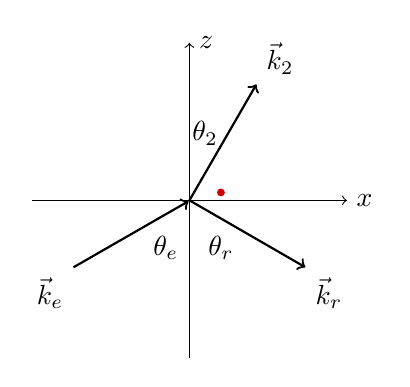
\begin{tikzpicture}
			\draw[->] (-2,0) -- (2,0) node[right] {$x$};
			\draw[->] (0,-2) -- (0,2) node[right] {$z$};
			\draw[thick,->] (0,0) -- (60:1.7cm) node[anchor=south west] {$\vec{k}_2$}; 
			\centerarc[](0,0)(60:90:1.2);
			\node at (0.2,.85) {$\theta_2$};
			\draw[thick,->] (-150:1.7cm) node[anchor=north east] {$\vec{k}_e$} -- (-0.01,-0.01);
			\draw[thick,->] (0,0) -- (-30:1.7cm) node[anchor=north west] {$\vec{k}_r$};
			\centerarc[](0,0)(210:270:1);
			\node at (-0.3,-0.6) {$\theta_e$};
			\centerarc[](0,0)(270:330:1);
			\node at (0.4,-0.6) {$\theta_r$};
			\centerarc[thick,black!20!red](0,0)(-30:60:.7cm);
			\node[circle,fill=black!20!red,inner sep=1pt,minimum size=1pt] at (.4,.1) {};
		\end{tikzpicture}
	\end{minipage}%
	\\
\end{enumerate}

\subsubsection{Einschub}

Nun noch eine Erklärung die etwas umständlicher ist: (Zu senkrechtem Einfall)\\
\begin{minipage}{.5\linewidth}
	$ \vec{E}_{e_0} = E_{e_0} \vec{e}_y $\\
	$ \vec{E}_{r_0} = E_{r_0} \vec{e}_y \quad \vec{E}_{2_0} = E_{2_0} \vec{e}_y $\\[5pt]
\end{minipage}%
\begin{minipage}{.5\linewidth}
	\flushright
	%t6:
	\begin{tikzpicture}[scale=.9]
		\draw[->] (-2.5,0) -- (2.5,0) node[right] {$x$};
		\draw[->] (0,-2.5) -- (0,2.5) node[right] {$z$};
		\draw[thick,->] (0,0) -- (30:2.5cm) node[anchor=south west] {$\vec{k}_2$}; 
		\centerarc[](0,0)(30:90:.9);
		\node at (0.3,.5) {$\theta_2$};
		\draw[thick,->] (-135:2.5cm) node[anchor=north east] {$\vec{k}_e$} -- (-0.01,-0.01);
		\node at (-0.2,-0.5) {$\theta_e$};
		\centerarc[](0,0)(-90:-45:.9);
		\draw[thick,->] (0,0) -- (-45:2.5cm) node[anchor=north west] {$\vec{k}_r$};
		\centerarc[](0,0)(-135:-90:.9);
		\node at (0.25,-0.5) {$\theta_r$};
		%E und B Felder
		\coordinate (2) at (30:1.5);
		\draw[black!20!red,thick] (2) circle (.15cm);
		\draw[black!20!red,thick] ($ (2) + (-135+30:.15) $) -- ++(45+30:.3);
		\draw[black!20!red,thick] ($ (2) + (135+30:.15) $) -- ++(-45+30:.3);
		\node[black!20!red,anchor=south east] at (2) {$ \vec{E}_2 $};
		%
		\coordinate (e) at (-135:1.5);
		\draw[black!20!red,thick] (e) circle (.15cm);
		\draw[black!20!red,thick] ($ (e) + (-135+45:.15) $) -- ++(45+45:.3);
		\draw[black!20!red,thick] ($ (e) + (135+45:.15) $) -- ++(-45+45:.3);
		\node[black!20!red,anchor=south east] at (e) {$ \vec{E}_e $};
		%
		\coordinate (r) at (-45:1.5);
		\draw[black!20!red,thick] (r) circle (.15cm);
		\draw[black!20!red,thick] ($ (r) + (-135+45:.15) $) -- ++(45+45:.3);
		\draw[black!20!red,thick] ($ (r) + (135+45:.15) $) -- ++(-45+45:.3);
		\node[black!20!red,anchor=south west] at (r) {$ \vec{E}_r $};
	\end{tikzpicture}
\end{minipage}%
\\
\begin{enumerate}
	\item[ii)] $ \vec{t} = \vec{e}_x: $
	\begin{equation*}
	0 = \vec{e}_x \cdot (\vec{E}_{2_0} - \vec{E}_{r_0} - \vec{E}_{e_0})
	\end{equation*}
	\begin{equation*}
	\Rightarrow \quad E_{2_{0_x}} = E_{r_{0_x}}
	\end{equation*}
	\item[i)]
	\begin{equation*}
	0 = \vec{e}_z \cdot (\epsilon_2 \vec{E}_{2_0} - \epsilon_1 \vec{E}_{r_0} - \epsilon_1 \vec{E}_{e_0})
	\end{equation*}
	\begin{equation*}
	\Rightarrow \quad \epsilon_2 E_{2_{0_z}} = \epsilon_1 E_{r_{0_z}}
	\end{equation*}
	$ \vec{k}_e, \vec{k}_r, \vec{k}_2 $ in $ x $-$ z $-Ebene
	\begin{equation*}
	\vec{k}_r = \begin{pmatrix}
	k_{r_x} \\ 0 \\ k_{r_z}
	\end{pmatrix} \qquad \vec{k}_2 = \begin{pmatrix}
	k_{2_x} \\ 0 \\ k_{2_z}
	\end{pmatrix}
	\end{equation*}
	\begin{align*}
	0 &= \vec{k}_r \cdot \vec{E}_{r_0} = k_{r_x} E_{r_{0_x}} + k_{r_z} E_{r_{0_z}} \quad \leftarrow \quad 0 = k_{r_x} E_{2_{0_x}} + k_{r_z} \frac{\epsilon_2}{\epsilon_1} E_{2_{0_z}} \\
	0 &= \vec{k}_2 \cdot \vec{E}_{2_0} = k_{2_x} E_{e_{0_x}} + k_{2_z} E_{2_{0_z}} \quad \rightarrow \quad E_{2_{0_x}} = - \frac{k_{r_z}}{k_{r_x}} \frac{\epsilon_2}{\epsilon_1} E_{2_{0_z}}
	\end{align*}
	\begin{equation*}
	\Rightarrow \quad 0 = \custo{\neq}{\left[- \cancel{k_{z_x}} \frac{k_{r_z}}{\cancel{k_{r_x}}} \frac{\epsilon_2}{\epsilon_1} + k_{2_z}\right]}{0} \equalto{E_{2_{0_z}}}{0}
	\end{equation*}
	$ k_{2_x} = k_{r_x} $
\end{enumerate}

% Vorlesung 17.01.18

\section{Aspekte der Absorption und Dispersion elektromagnetischer Felder}

bisher galt: freie Ausbreitung der EM-Wellen\\
in Medien gilt:\\[5pt]
\begin{minipage}{.5\linewidth}
	\textbf{Absorption:} 
\end{minipage}%
\begin{minipage}{.5\linewidth}
	$ \ \, $ und \textbf{Dispersion:}
\end{minipage}%
\\
\begin{minipage}{.5\linewidth}
	\flushleft
	%t1:
	\begin{tikzpicture}[xscale=.75,scale=.8]
		\fill[gray!10!] (0,-1.5) rectangle (6.3,1.5);
		\fill[pattern=north east lines,pattern color = gray!50!] (0,-1.5) rectangle (6.3,1.5);
		\draw[thick] (0,-1.5) -- (0,1.5);
		\draw[domain=-4.725:0, samples=100, thick] plot (\x, {sin((\x * 4) r)});
		\draw[domain=0:6.3, samples=100, thick] plot (\x, {sin((\x * 4) r) * exp(-\x * 0.4)});
	\end{tikzpicture}
\end{minipage}%
\begin{minipage}{.5\linewidth}
	\flushright
	%t2:
	\begin{tikzpicture}[scale=1.05]
		\draw[fill=gray!10!] (0,0) -- ++(-60:2cm) -- ++(-180:2cm) -- cycle;
		\draw[<-, thick] (-120:1cm) -- ++(-160:2cm) node[left] {$ h(\omega) , \epsilon(\omega) $};
		\foreach \x\a\l in {.4/5/1, .5/-7.5/2, .6/-20/3}
		\draw[->, thick] ($ (0,0)!\x!(-60:2cm) $) -- ++(\a:2cm) node[right] {$ \omega_{\l} $};
	\end{tikzpicture}
\end{minipage}%

\subsection{Elektromagnetische Wellen in elektrischen Leitern}

bisher galt: \textbf{Isolator/Vakuum} freie Ladungen und freie Ströme = 0 $\qquad \rho_f = 0 = \vec{j}_f $\\
im Leiter gilt: \textbf{Ohmsche Leiter} $ \vec{j} = \sigma \vec{E}  \qquad \rho = 0 \qquad \sigma : $ Leitfähigkeit
\begin{equation*}
\vec{D} = \epsilon \vec{E} \qquad \vec{B} = \mu \vec{H}
\end{equation*}
Maxwell-Gleichungen:
\begin{align*}
\vabla \cdot \vec{E} &= 0 \qquad \qquad \qquad \ \, \vabla \cdot \vec{B} = 0\\
\vabla \times \vec{E} + \prt{\vec{B}}{t} &= 0 \qquad \vabla \times \vec{B} - \mu \epsilon \prt{\vec{E}}{t} = \mu \vec{j} = \mu \sigma \vec{E}
\end{align*}
\emph{Bemerkung:}\\
$ \vabla \cdot \vec{E} = \frac{1}{\epsilon_0} \rho $\\
$ \prt{\rho}{t} = - \vabla \vec{j} = - \sigma \vabla \vec{E} = - \frac{\sigma}{\epsilon} \rho $\\
$ \rho(\vec{r},t) = e^{-\frac{\sigma}{\epsilon} t} \rho(\vec{r},t=0) $\\
somit ist die Annahme $ \rho = 0 $ gerechtfertigt.\\[15pt]
\begin{align*}
0 &= \vabla \times (\vabla \times \vec{E}) + \prt{}{t} (\vabla \times \vec{B}) \\
&= \vabla (\cancel{\vabla \vec{E}}) - \Delta \vec{E} + \prt{}{t} (\mu \epsilon \prt{\vec{E}}{t} + \mu \sigma \vec{E})
\end{align*}
\begin{equation*}
\Rightarrow \quad \rmbox{\Delta \vec{E} - \mu \epsilon \prt{^2 \vec{E}}{t^2} - \mu \sigma \prt{\vec{E}}{t} = 0}
\end{equation*}
Analog kann man auch nach $ \Delta \vec{B} $ auflösen:
\begin{equation*}
\Rightarrow \quad \rmbox{\Delta \vec{B} - \mu \epsilon \prt{^2 \vec{B}}{t^2} - \mu \sigma \prt{\vec{B}}{t} = 0}
\end{equation*}
Diese Beiden Gleichungen nennt man auch \textbf{Telegraphen-Gleichungen}.\\[5pt]
Ansatz zur Lösung: monochromatische, ebene Welle $ \qquad \vec{k} = k \vec{e}_z $
\begin{align*}
\vec{E}(\vec{r},t) &= \vec{E}_0 e^{i(\vec{k} \cdot \vec{r} - \omega t)} = \vec{E}_0 e^{i(k r - \omega t)}\\
\vec{B}(\vec{r},t) &= \vec{B}_0 e^{i(k r - \omega t)}
\end{align*}
\begin{equation*}
\Rightarrow \quad 0 = - k^2 + \mu \epsilon \omega^2 + i \omega \mu \sigma = - k^2 + \mu \omega^2 \ub{( \epsilon + i \frac{\sigma}{\omega})}_{\eqdef \eta}
\end{equation*}
$ \eta : $ \textbf{verallgemeinerte Dielektrizitätskonstante}
\frbox{Dispersionsrelation im leitenden Medium ($ k(\omega) $)}{
\begin{equation*}
\Rightarrow \quad k^2 = \mu \eta \omega^2 = \mu \omega^2 \left(\epsilon + i \frac{\sigma}{\omega}\right)
\end{equation*}
}
\noindent
Hieraus folgt, dass $ \vec{k} $ komplex ist und einen Imaginärteil haben muss: $ k = k_{R} + i k_{I} $
\begin{align*}
\Rightarrow \quad k^2 &= k_R^2 - k_I^2 + 2 i k_R k_I\\
&\overset{!}{=} \mu \epsilon \omega^2 + i \mu \sigma \omega
\end{align*}
\begin{equation*}
\Rightarrow \quad k_{R/I} = \omega \sqrt{\frac{\epsilon \mu}{2}} \left[\sqrt{1 + \left(\frac{\sigma}{\epsilon \omega}\right)^2} \pm 1\right]^{\frac{1}{2}}
\end{equation*}
\begin{align*}
\vec{E} &= \vec{E}_0 e^{i(k z - \omega t)} \\
&= \vec{E}_0 e^{i((k_R + i k_I) z - \omega t)} \\
&= \vec{E}_0 e^{-k_I z} e^{i(k_R z - \omega t)}
\end{align*}
\begin{minipage}{.4\linewidth}
	\textbf{Eindringtiefe:} $ d = \frac{1}{k_I} $\\[10pt]
	typische Werte:\\
	Kupfer: $ \sigma = 5{,}81 \cdot 10^{7} \ \frac{1}{\Omega \tx{m}} $\\
	\begin{tabular}{c|c}
		$ \nu $ & $ d $ \\
		\hline
		1 MHz & 66 $ \mu $m \\
		$ 6 \cdot 10^{14} $ Hz & 2,7 nm
	\end{tabular}\\[15pt]
\end{minipage}%
\begin{minipage}{.6\linewidth}
	\flushright
	%t3:
	\begin{tikzpicture}[xscale=.8]
		\fill[gray!10!] (0,-1.5) rectangle (6.3,1.5);
		\fill[pattern=north east lines,pattern color = gray!50!] (0,-1.5) rectangle (6.3,1.5);
		\draw[thick,->] (0,-1.7) -- (0,1.7);
		\draw[thick,->] (-5,0) -- (6.7,0);
		\draw[domain=-4.725:0, samples=100, thick] plot (\x, {sin((\x * 4) r)});
		\draw[domain=0:6.3, samples=100, thick] plot (\x, {sin((\x * 4) r) * exp(-\x * 0.5)});
		\draw[domain=0:6.3, samples=100, thick, dashed] plot (\x, {exp(- \x * 0.5)});
		\draw (2.5,.5) to[out=40,in=-180] (3.5,1) node[right, fill=white, opacity=.8, rounded corners=5pt] {$ \propto e^{- i k z} $};
	\end{tikzpicture}
\end{minipage}%
\\
\emph{Bemerkung:}
\lcom{Man kann Zeigen, dass, anders als im Vakuum, im Medium das $ \vec{B} $-Feld Phasenverschoben zum $ \vec{E} $-Feld ist. Wir werden hierauf aus Zeitgründen nicht genauer eingehen.}

\subsection{Frequenzabhängigkeit der Dielektrizitätskonstanten - Dispersion}

\subsubsection{Modell für $ \epsilon(\omega) $}

Wir betrachten hier nicht magnetisierbare Medien. Es soll gehen $ \mu_r \approx 1 $.
\begin{equation*}
\epsilon = \epsilon_0 (1 + \chi_e) \qquad \vec{P} = \epsilon_0 \chi_e \vec{E} = \frac{\tx{Dipole}}{\tx{Volumen}} = N \langle \vec{p} \rangle
\end{equation*}
\lcom{Die Polarisation ist die mittlere Dipol-dichte pro Volumen.}\\[5pt]
Die Verschiebungsolarisation ist:
\begin{equation*}
\langle \vec{p} \rangle = \alpha \vec{E}
\end{equation*}
$ \alpha : $ atomare Polarisierbarkeit
\begin{equation*}
\chi_e = \frac{N \alpha}{\epsilon_0}
\end{equation*}
$ \chi_e : $ elektrische Suszeptibilität\\
All diese Gleichungen würde man für langsam schwingende Felder erhalten also für $ \omega \to 0 $.\\
\lcom{Bei Tieffrequenten Wellen können die Ladungen den Feldern folgen und schwächen diese dadurch ab. Bei Hochfrequenten Wellen können die Ladungen den Feldern nicht mehr folgen und der Effekt ist ein anderer.}

\subsubsection{Klassisches Oszillatormodell für die Bindung von Elektronen in Atomen}

\begin{center}
	%t4:
	\begin{tikzpicture}
		\draw[domain=-3.15:3.15, samples=250, thick, draw=gray!70!] plot(\x, {1.5 * sin(\x * 8 r)});
		\node at (2,-.7) {$ \vec{E}(\vec{r},t) $};
		\coordinate (p) at (-1.5,-.8);
		\coordinate (m) at (1.5,.8);
		\draw[decorate,decoration={aspect=.5, segment length=4mm, amplitude=.5cm,coil},thick] ($ (p) + (30:0.15) $) -- ($ (m) + (30:0.15) $);
		\node[circle,draw=black,fill=black!10!red] at (p) {$ + $};
		\node[circle,draw=black,fill=black!10!blue] at (m) {$ - $};
		\draw[thick,->] ($ (p) + (120:.8) $) -- node[above,xshift=2pt] {$ \vec{r} $} ($ (m) + (120:.8) $);
	\end{tikzpicture}
\end{center}
$ \omega_0 : $ Frequenz\\
$ \gamma : $ Dämpfung\\
Dies können wir durch einen getriebenen, gedämpften, harmonischen Oszillator darstellen:
\begin{equation*}
m(\ddot{\vec{r}} + \gamma \dot{\vec{r}} + \omega_0^2 \vec{r}) = q \vec{E}(\vec{r},t)
\end{equation*}
$ \rightarrow $ Dipolmoment: $ \vec{p} = q \vec{r} \qquad q = -e $
\begin{equation*}
\Rightarrow \quad m(\ddot{\vec{p}} + \gamma \dot{\vec{p}} + \omega_0^2 \vec{p}) = e^2 \vec{E}
\end{equation*}
\textbf{statischer Grenzfall:} $ \vec{E}(\vec{r},t) = \vec{E}(\vec{r}) $\\
$ \Rightarrow \quad \dot{\vec{p}} = 0 = \ddot{\vec{p}} $\\
\begin{equation*}
\Rightarrow \quad \vec{p} = \frac{e^2 \vec{E}}{m \omega_0^2} = \alpha \vec{E} \quad \rightarrow \quad \alpha = \frac{e^2}{m \omega_0^2}
\end{equation*}
\begin{equation*}
\Rightarrow \quad \chi_e = \frac{N e^2}{\epsilon_0 m \omega_0^2}
\end{equation*}
\textbf{zeitabhängiger Fall:} $ \vec{E} = \vec{E}_0 e^{-i \omega t} \qquad e^{ikz} = e^{i \frac{2 \pi}{\lambda} z} $\\[5pt]
Mechanik:\\
$ \Rightarrow \quad \vec{p}(t) : $ erzwungene Schwingung mit Frequenz $ \omega $
\begin{equation*}
\vec{p}(t) = \vec{p}_0 e^{- i \omega t}
\end{equation*}
\begin{equation*}
m ( - \omega^2 - i \gamma \omega + \omega_0^2) \vec{p}_0 e^{-i \omega t} = e^2 \vec{E}_0 e^{-i \omega t}
\end{equation*}
\begin{equation*}
\Rightarrow \quad \vec{p}_0 = \ub{\frac{e^2}{m} \frac{1}{\omega_0^2 - \omega^2 - i \gamma \omega}}_{\alpha (\omega)} \vec{E}_0
\end{equation*}
\begin{align*}
\Rightarrow \quad \chi_e(\omega) &= \frac{N \alpha(\omega)}{\epsilon_0} \\
&= \frac{N e^2}{\epsilon_0 m} \frac{1}{\omega_0^2 - \omega^2 - i \gamma \omega}
\end{align*}
\begin{align*}
\Rightarrow \quad \epsilon(\omega) &= \epsilon_0 \epsilon_r(\omega) \\
&= \epsilon_0 (1 + \chi_e(\omega))
\end{align*}
\frbox{Dispersionsrelation im leitenden Medium $ \epsilon_r(\omega) $}{
\begin{equation*}
\epsilon_r(\omega) = 1 + \frac{N e^2}{\epsilon_0 m} \frac{1}{\omega_0^2 - \omega^2 - i \gamma \omega}
\end{equation*}
}
\noindent
Realteil:
$$ \Re(\epsilon_r(\omega)) = 1 + \frac{Ne^2}{\epsilon_0 m} \frac{\omega_0^2 - \omega^2}{(\omega_0^2 - \omega^2)^2 + \gamma^2 \omega^2} $$
Imaginärteil:
$$ \Im(\epsilon_r(\omega)) = \frac{N e^2}{\epsilon_0 m} \frac{\gamma \omega}{(\omega_0^2 - \omega^2)^2 + \gamma^2 \omega^2} \quad \ \  $$
\begin{minipage}{.5\linewidth}
	%t5:
	\begin{tikzpicture}[scale=.7]
		\draw[->] (-.1,0) -- (8,0) node[anchor=north west] {$ \omega $};
		\draw[->] (0,-.1) node[below] {$ 0 $} -- (0,5) node[left] {$ \Re(\epsilon_r(\omega)) $};
		\coordinate (R) at (0,4);
		\coordinate (w) at (3,0);
		\node[left] at (R) {$ \Re(\epsilon_r(0)) $};
		\node[below] at ($ (w) + (-.1,0) $) {$ \omega_0 $};
		\draw ($ (R) + (-.1,0) $) -- ++(.2,0);
		\draw ($ (w) + (0,-.1) $) -- ++(0,.2);
		\draw (-.1,1.5) node[left] {1} -- ++(.2,0);
		%\draw[thick,looseness=.8] (R) to[out=0,in=-135] (1.5,2.8) to[out=45,in=-180] (2.5,3.8) to[out=0,in=100] (3,1.75);
		%\draw[thick,looseness=1] (R) to[out=0,in=-135] (2.2,5) to[out=45,in=100] (2.8,5.8) to[out=-80,in=100] (3.2,0.2);
		%\draw[domain=0:5, samples=100, thick] plot (\x, {(10 * (\x)) / ((4 - (\x)^2)^2 + 2 * (\x)^2))});
		\draw[domain=0:8, samples=100, thick] plot (\x, {0.5 + 1 +  10 * (  4 - (\x * 0.668)^2) / ((4 - (\x * 0.668)^2)^2+ 2 * (\x * 0.668)^2)});
		\draw[thick,dashed] (0,1.5) -- (8,1.5);
		\draw[thick,dashed] (w) -- ++(0,2);
		\draw[dashed] (1.7,0) -- ++(0,5);
		\draw[dashed] (3.7,0) -- ++(0,5);
		\node at (.9,5.5) {\small normal};
		\node at (2.7,6) {\small anormal};
		\node at (4.5,5.5) {\small normal};
		\node at (7,5.8) {\small Dispersion};
	\end{tikzpicture}
	\begin{comment} % alternative:
	\begin{tikzpicture}
		\draw[scale=1.5,red,line width=1,domain=-2:2, samples=500] plot (\x, {((2 * \x) / (\x - 10  * ((\x)^2) - 0.25))});
		\coordinate (a) at (-3,-1.5);
		\coordinate (b) at (0,0);
		% Koordianten Achsen
		\draw[->] (a) -- ++(6,0) node[right] {$\omega$};
		\draw[->] (a) -- ++(0,3) node[left] {$Re(\epsilon(\omega)$};
		\node[left] at ($(a) + (0,1.8)$) {$Re(\epsilon(0)$};
		%Unterteilung
		\draw[dashed] ($ (a) + (0,1.36) $) node[left] {$1$} -- ++(6,0);
		\draw[dashed] (0,-1.6) node[below] {$\omega_0$} -- (0,0);
		\draw[dashed] ($ (b) + (0.25,-1.8) $)  -- ++(0,3);
		\draw[dashed] ($ (b) + (-0.25,-1.8) $) -- ++(0,3);
		%Beschriftung
		\node at (-2,1) {normal};
		\node at (2.5,1) {normale Dispersion};
		\node at (0,1.5) {anormal};
	\end{tikzpicture}\\
	\end{comment}
	\vspace{5pt}
\end{minipage}%
\begin{minipage}{.5\linewidth}
	\flushright
	\vspace{5pt}
	%t6:
	\begin{tikzpicture}[scale=.7]
		\draw[->] (-.1,0) -- (8,0) node[anchor=north west] {$ \omega $};
		\draw[->] (0,-.1) node[below] {$ 0 $} -- (0,5) node[anchor=south east] {$ \Im(\epsilon_r(\omega)) $};
		\coordinate (w) at (3,0);
		\node[below,yshift=-3pt] at ($ (w) + (-.1,0) $) {$ \omega_0 $};
		\draw ($ (w) + (0,-.1) $) -- ++(0,.2);
		%\draw[thick,looseness=.8] (R) to[out=0,in=-135] (1.5,2.8) to[out=45,in=-180] (2.5,3.8) to[out=0,in=100] (3,1.75);
		%\draw[thick,looseness=1] (R) to[out=0,in=-135] (2.2,5) to[out=45,in=100] (2.8,5.8) to[out=-80,in=100] (3.2,0.2);
		\draw[domain=0:8, samples=100, thick] plot (\x, {(13 * (\x * 0.63)) / ((4 - (\x * 0.63)^2)^2 + 2 * (\x * 0.63)^2))});
		%\draw[domain=0:8, samples=100, thick] plot (\x, {0.5 + 1 +  10 * (  4 - (\x * 0.668)^2) / ((4 - (\x * 0.668)^2)^2+ 2 * (\x * 0.668)^2)});
		\draw[dashed, thick] (w) -- ++(0,4);
	\end{tikzpicture}
\end{minipage}%
\\
\emph{Bemerkung:} \textbf{Dispersion}\\
Frequenzabhängigkeit von $ \epsilon = \epsilon (\omega) = \epsilon_R + i \epsilon_I $\\
Brechungsindex $ n = \sqrt{\epsilon_r \mu_r} = n (\omega) $\\
normale Dispersion: $ \prd{\epsilon_R}{\omega} > 0 $\\
anormale Dispersion: $ \prd{\epsilon_R}{\omega} < 0 $\\[5pt]
\begin{minipage}{.5\linewidth}
	\textbf{Verallgemeinert auf $ j $ Elektronen}\\
	\textbf{im Atom:}\\
	$ f_j : $ Elektronen mit Frequenz $ \omega_j , \gamma_j $
	\begin{equation*}
	\epsilon_r(\omega) = 1 + \frac{N e^2}{\epsilon_0 m} \sum_j \frac{f_j}{\omega_j^2 - \omega^2 - i \gamma_j \omega_j}
	\end{equation*}
\end{minipage}%
\begin{minipage}{.5\linewidth}
	\flushright
	%t7:
	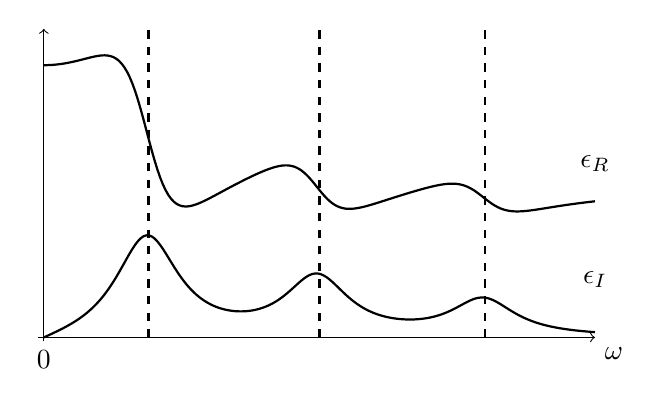
\begin{tikzpicture}[yscale=.7,scale=.7]
		\draw[->] (-.1,0) -- (10,0) node[anchor=north west] {$ \omega $};
		\draw[->] (0,-.1) node[below] {$ 0 $} -- (0,8);
		
		\draw[domain=0:10, samples=200, thick] plot (\x, {3 + 1 +  10 * (4 - (\x)^2) / ((4 - (\x)^2)^2 + 2 * (\x)^2) +  10 * (25  - (\x)^2) / ((25 - (\x)^2)^2 + 2 * (\x)^2) + 10 * (64 - (\x)^2) / ((64 - (\x)^2)^2 + 2 * (\x)^2});
		%1 +  10 * (4 - (\x)^2) / ((4 - (\x)^2)^2 + 2 * (\x)^2)
		%1 +  10 * (4 - (\x)^2) / ((4 - (\x)^2)^2 + 2 * (\x)^2) +  15 * ( 49  - (\x)^2) / ((49 - (\x)^2)^2 + 2 * (\x)^2) + 10 * (144 - (\x)^2) / ((144 - (\x)^2)^2 + 2 * (\x)^2)
		
		\draw[domain=0:10, samples=200, thick] plot (\x, {(10 * (\x)) / ((4 - (\x)^2)^2 + 2 * (\x)^2) +  (15 * (\x)) / ((25 - (\x)^2)^2 + 2 * (\x)^2) +  (15 * (\x)) / ((64 - (\x)^2)^2 + 2 * (\x)^2)});
		%(10 * (\x)) / ((4 - (\x)^2)^2 + 2 * (\x)^2) +  (15 * (\x)) / ((49 - (\x)^2)^2 + 2 * (\x)^2) + (10 * (\x)) / ((144 − (\x)^2)^2 + 2 * (x)^2)
		%\draw[domain=0:8, samples=500, thick] plot (\x, {0.5 + 1 +  10 * (  4 - (\x * 0.668)^2) / ((4 - (\x * 0.668)^2)^2+ 2 * (\x * 0.668)^2)});
		
		\foreach \x in {1.9,5,8}
		\draw[thick,dashed] (\x,0) -- ++(0,8);
		\node at (10,1.5) {$ \epsilon_{I} $};
		\node at (10,4.5) {$ \epsilon_{R} $};
	\end{tikzpicture}
	\vspace{10pt}
\end{minipage}%
\\
\begin{minipage}{.5\linewidth}
	Die Quantenmechanik erklärt diese\\
	Sprünge durch Energieniveaus:\\
\end{minipage}%
\begin{minipage}{.5\linewidth}
	%t8:
	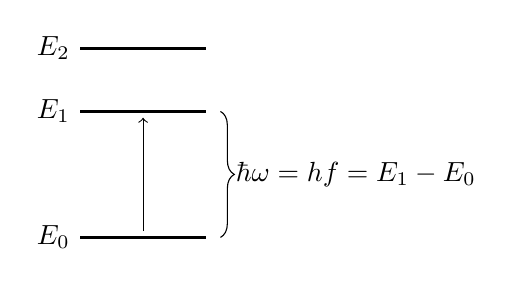
\begin{tikzpicture}[scale=.8]
		\foreach \y\l in {0/0, 2/1, 3/2}
		\draw[thick] (0,\y) node[left] {$ E_{\l} $} -- ++(2,0);
		\draw[->] (1,.1) -- ++(0,1.8);
		\draw[decorate, decoration={brace,amplitude=5pt,mirror,raise=2pt}, xshift=4pt,black] (2,0) -- node[right,xshift=4pt] {$ \hbar \omega = h f = E_1 - E_0 $} (2,2);
	\end{tikzpicture}
\end{minipage}

\subsection{Bedeutung der komplexen/frequenzabhängigen Dielektrizitäts- \texorpdfstring{\\}{zeilenumbruch} konstante}

Wellengleichung im Medium $ \quad \epsilon = \epsilon(\omega) \quad \mu \approx \mu_0 \quad \sigma = 0 $
\begin{equation*}
\Delta \vec{E} - \mu_0 \epsilon \prt{^2 \vec{E}}{t^2} = 0
\end{equation*}
\begin{equation*}
\qquad \qquad \qquad \qquad \qquad \qquad \vec{E} = \vec{E}_0 e^{i(kz - \omega t)} \begin{tikzpicture}[scale=.7]
\draw[thick, ->] (0,0) -- (1,0) -- (1,1);
\end{tikzpicture}\qquad \quad \Big| \quad - k^2 + \mu_0 \epsilon \omega^2 = 0 \ \
\end{equation*}
\begin{equation*}
\Rightarrow \quad k^2 = \mu_0 \epsilon \omega^2 = \mu_0 (\epsilon_R + i \epsilon_I) \omega^2
\end{equation*}
$ k = k_R + i k_I $
\begin{equation*}
k_R^2 - k_I^2 + 2 i k_R k_I = \mu_0 \epsilon_R \omega^2 + i \mu_0 \epsilon_I \omega^2
\end{equation*}
\begin{equation*}
k_{R/I} = \omega \sqrt{\frac{\mu_0 \epsilon_R}{2}} \left[\sqrt{1 + \left(\frac{\epsilon_I}{\epsilon_R}\right)^2} \pm 1\right]^{\frac{1}{2}}
\end{equation*}
\begin{equation*}
\epsilon_I \approx 0 \quad k_I \approx 0 \quad k_R \approx \omega \sqrt{\mu_0 \epsilon_R(\omega)}
\end{equation*}
\begin{minipage}{.5\linewidth}
	\begin{equation*}
	\Rightarrow \quad \vec{E}(\vec{r},t) = \vec{E}_0 e^{- k_I z} e^{i(k_R z - \omega t)}
	\end{equation*}
\end{minipage}%
\begin{minipage}{.5\linewidth}
	\flushright
	%t9:
	\begin{tikzpicture}[xscale=.75, scale=.8]
		\fill[gray!10!] (0,-1.5) rectangle (6.3,1.5);
		\fill[pattern=north east lines,pattern color = gray!50!] (0,-1.5) rectangle (6.3,1.5);
		\draw[thick] (0,-1.5) -- (0,1.5);
		\draw[domain=-4.725:0, samples=100, thick] plot (\x, {sin((\x * 4) r)});
		\draw[domain=0:6.3, samples=100, thick] plot (\x, {sin((\x * 4) r) * exp(-\x * 0.4)});
	\end{tikzpicture}
\end{minipage}%
\\
Ausbreitungsgeschwindigkeit:
$$ v = \frac{\omega}{k_R} = v(\omega) = \frac{c}{n(\omega)} $$

%Vorlesung 21.01. Vertretung von Prof Thoss

\section{Allgemeine Lösung der Maxwell-Gl. - Retardierte Potentiale}

Wir suchen Lösungen der Gleichungen:
\begin{align*}
\vabla \cdot \vec{B} &= 0 \qquad \qquad \quad \vabla \times \vec{E} + \prt{\vec{B}}{t} = 0\\
\vabla \cdot \vec{E} &= \frac{1}{\epsilon_0} \rho \qquad \qquad \vabla \times \vec{B} - \ub{\epsilon_0 \mu_0}_{\frac{1}{c^2}} \prt{\vec{E}}{t} = \mu_0 \vec{j}
\end{align*}
gegeben: $ f(\vec{r},t) , \vec{j}(\vec{r},t) $\\
gesucht: $ \vec{E}(\vec{r},t), \vec{B}(\vec{r},t) $\\[5pt]
zur formalen Lösung der Gleichungen verwenden wir die Potentiale $ \Phi , \vec{A} $ der Elektrodynamik
\begin{equation*}
\vec{B} = \vabla \times \vec{A} \qquad \qquad \vec{E} = - \vabla \Phi - \prt{\vec{A}}{t}
\end{equation*}
\textbf{Lorenzeichung:}
\begin{equation*}
\vabla \cdot \vec{A} + \frac{1}{c^2} \prt{\Phi}{t} = 0
\end{equation*}
Aus den inhomogenen Gleichungen erhalten wir die entkoppelten Wellengleichungen der Potentiale:
\begin{equation*}
\Delta \Phi - \frac{1}{c^2} \prt{^2 \Phi}{t^2} = - \frac{1}{\epsilon_0} \rho
\end{equation*}
\begin{equation*}
\Delta \vec{A} - \frac{1}{c^2} \prt{^2 \vec{A}}{t^2} = - \mu_0 \vec{j}
\end{equation*}
\emph{Nebenbemerkung:}
\begin{equation*}
\Delta \Psi (\vec{r},t) - \frac{1}{c^2} \prt{^2}{t^2} \Psi (\vec{r},t) \eqdef \square \Psi (\vec{r},t)
\end{equation*}
mit $ \square : $ \textbf{d'Alembert Operator}
\begin{equation*}
\square = \Delta - \frac{1}{c^2} \prt{^2}{t^2}
\end{equation*}
Aus der Elektro-/Magnetostatik ist bekannt:
\begin{equation*}
\prt{}{t} \Phi = 0 = \prt{}{t} \vec{A}
\end{equation*}
\begin{align*}
\Delta \Phi(\vec{r}) &= - \frac{1}{\epsilon_0} \rho \qquad \tx{ Poisson-Gleichung}\\
\Delta \vec{A}(\vec{r}) &= - \mu_0 \vec{j}
\end{align*}
Die Lösungen waren:
\begin{equation*}
\Phi(\vec{r}) = \Phi_{\tx{hom}}(\vec{r}) + \Phi_{\tx{inh}}(\vec{r})
\qquad \qquad
\tx{mit}
\qquad 
\Phi_{\tx{inh}}(\vec{r}) = \kq \int \dd^3 \vec{r}' \frac{\rho(\vec{r}')}{| \vec{r} - \vec{r}' |}
\end{equation*}
sowie für das Vektorpotential:
\begin{equation*}
\vec{A}(\vec{r}) = \vec{A}_{\tx{hom}} (\vec{r}) + \vec{A}_{\tx{inh}} (\vec{r})
\qquad \qquad 
\tx{mit}
\qquad
\vec{A}_{\tx{inh}} (\vec{r}) = \frac{\mu_0}{4 \pi} \int \dd ^3 \vec{r}' \frac{\vec{j}(\vec{r})}{| \vec{r} - \vec{r}' |}
\end{equation*}
und $ \Delta \vec{A}_{\tx{hom}}(\vec{r}) = 0 $\\[10pt]
Wir können die Diskussion auf das skalare Potential $ \Phi $ beschränken:
\begin{equation*}
\Delta \Phi - \frac{1}{c^2} \prt{^2}{t^2} \Phi = - \frac{1}{\epsilon_0} \rho
\end{equation*}
$ \Phi(\vec{r},t) = \Phi_{\tx{hom}} + \Phi_{\tx{inh}} $\\
wobei:\\
$ \Phi_{\tx{hom}} : $ allgemeine Lösung der homogenen DGL $ \Delta \Phi_{\tx{hom}} - \frac{1}{c^2} \prt{^2}{t^2} \Phi_{\tx{hom}} = 0 $ \\
$ \Phi_{\tx{inh}} : $ \ \, spezielle Lösung der inhomogenen DGL $ \Delta \Phi_{\tx{inh}} - \frac{1}{c^2} \prt{^2}{t^2} \Phi_{\tx{inh}} = - \frac{1}{\epsilon_0} \rho $\\[5pt]
Lösung der homogenen Wellengleichung liefert z.B. Kugelwellen oder ebene Wellen:
\begin{equation*}
\Phi_{\tx{hom}}(\vec{r},t) = \Re \left\{ a e^{i(\vec{k} \cdot \vec{r} - \omega t)} \right\}
\end{equation*}
mit $ \vec{k} \in \mathbb{R}^3 $, $ |\vec{k}| = \frac{\omega}{c} $ bzw.: $ \omega(\vec{k}) = |\vec{k}| c $\\[5pt]
Die allgemeine Lösung erhalten wir nun durch Linearkombination:
\begin{equation*}
\Phi_{\tx{hom}}(\vec{r},t) = \Re \left\{ \int \dd ^3 \vec{k} \ a (\vec{k}) e^{i (\vec{k} \cdot \vec{r} - \omega(\vec{k}) t)} \right\}
\end{equation*}
Bestimmung einer speziellen Lösung der inhomogenen Wellengleichung:
\begin{equation*}
\Delta \Phi - \frac{1}{c^2} \prt{^2}{t^2} \Phi = - \frac{1}{\epsilon_0} \rho
\end{equation*}
zur Lösung der DGL betrachten wir eine Fouriertransformation von $ \Phi (\vec{r},t) $ bezüglich der Variablen $ t $.
\begin{equation*}
\tilde{\Phi}(\vec{r},\omega) \defeq \frac{1}{\sqrt{2 \pi}} \int_{- \infty}^{\infty} \dd t \Phi (\vec{r},t) e^{i \omega t}
\end{equation*}
Man kann danach zurücktransformieren:
\begin{equation*}
\Phi (\vec{r},t) = \frac{1}{\sqrt{2 \pi}} \int_{-\infty}^{\infty} \dd \omega \tilde{\Phi} (\vec{r},t) e^{- i \omega t}
\end{equation*}
wir können dies nun ineinander einsetzen um zu sehen ob dasselbe wieder herauskommt oder ob wir bei der Berechnung etwas verloren haben.
\begin{align*}
\Phi(\vec{r},t) &= \frac{1}{\sqrt{2 \pi}} \int_{- \infty}^{\infty} \dd \omega \left\{ \frac{1}{\sqrt{2 \pi}} \int_{- \infty}^{\infty} \dd t' \Phi(\vec{r},t) e^{i \omega t}\right\} e^{- i \omega t} \\
&= \int_{- \infty}^{\infty} \dd t' \Phi(\vec{r},t) \ub{\frac{1}{2 \pi} \int_{-\infty}^{\infty} \dd \omega e^{i \omega (t - t')}}_{= \delta(t - t')}\\
&= \Phi (\vec{r},t)
\end{align*}
Somit haben wir keine Information gewonnen oder erzeugt. Wir haben den Ausdruck lediglich in eine andere Darstellung umgeformt.\\[5pt]
Wir setzen nun die Fourierdarstellung in die DGL ein:
\begin{align*}
\prt{^2}{t^2} \Phi(\vec{r},t) &= \frac{1}{\sqrt{2 \pi}} \int \dd \omega \ \tilde{\Phi} (\vec{r},t) \ub{\prt{^2}{t^2} e^{- i \omega t}}_{= - \omega^2 e^{- i \omega t}}\\
&= \frac{1}{\sqrt{2 \pi}} \int \dd \omega (- \omega ^2) \tilde{\Phi} (\vec{r},t) e^{- i \omega t}
\end{align*}
Damit gilt:
\begin{align*}
& \frac{1}{\sqrt{2 \pi}} \int \dd \omega e^{- i \omega t} \left(\Delta + \frac{\omega^2}{c^2}\right) \tilde{\Phi} (\vec{r},t) = - \frac{1}{\epsilon_0} \rho (\vec{r},t)\\
\overset{\substack{\tx{Fouriertrafo.} \\ \tx{von } \rho}}{=} & \frac{1}{\sqrt{2 \pi}} \int \dd \omega e^{- i \omega t} \left(- \frac{1}{\epsilon_0}\right) \tilde{\rho} (\vec{r},\omega)
\end{align*}
\frbox{Helmholtz-Gleichung}{
\begin{equation*}
\Rightarrow \quad \left(\Delta + \frac{\omega^2}{c^2}\right) \tilde{\Phi} (\vec{r},t) = - \frac{1}{\epsilon_0} \tilde{\rho} (\vec{r},\omega)
\tag{*}
\label{Helmholtz}
\end{equation*}
}

\noindent
Zur Bestimmung der Lösung von \eqref{Helmholtz} betrachten wir zunächst eine Analogie zur Elektrostatik: $ \omega \to 0 \quad (\widehat{=} \ \prt{}{t} = 0) $
\begin{equation*}
\Rightarrow \quad \Delta \tilde{\Phi} = - \frac{1}{\epsilon_0} \tilde{\rho} \qquad \tx{Poisson-Gleichung}
\end{equation*}
spezielle Lösung (ohne Randbedingungen)
\begin{equation*}
\tilde{\Phi} (\vec{r},\omega = 0) = \kq \int \dd^3 r' \frac{\rho(\vec{r}')}{| \vec{r} - \vec{r}' |} = \int \dd^3 r' \grr \rho(\vec{r}')
\end{equation*}
mit der Green'schen Funktion:
\begin{equation*}
\grr = \kq \frac{1}{| \vec{r} - \vec{r}' |}
\end{equation*}
Diese erfüllt die Laplace Gleichung:
\begin{equation*}
\Delta_{\vec{r}} \grr = - \frac{1}{\epsilon_0} \delta(\vec{r} - \vec{r}')
\end{equation*}
Wir benötigen eine Verallgemeinerung für $ \omega \neq 0 $:
\begin{equation*}
\left(\Delta_{\vec{r}} + \frac{\omega^2}{c^2}\right) \gre_{\omega} (\vec{r}, \vec{r}') = - \frac{1}{\epsilon_0} \delta(\vec{r} - \vec{r}')
\end{equation*}
Es zeigt sich, dass gilt:
\begin{equation*}
\left(\Delta_{\vec{r}} + \frac{\omega^2}{c^2}\right) \kq \frac{e^{\pm i k |\vec{r} - \vec{r}'|}}{|\vec{r} - \vec{r}'|} = - 4 \pi \delta(\vec{r} - \vec{r}') = \grr
\end{equation*}
%
%
%
% oben stand Grr = - 4 \pi \delta (shit) aber es sollte glaub ich sein Grr = - 1/\epsilon_0 \delta(shit)
%
%
%
Mit $ k = \frac{\omega}{c} $ folgt daraus:
\begin{equation*}
\left(\Delta_{\vec{r}} + \frac{\omega^2}{c^2}\right) \kq \frac{e^{\pm i \frac{\omega}{c} |\vec{r} - \vec{r}'|}}{|\vec{r} - \vec{r}'|} = - \frac{1}{\epsilon_0} \delta(\vec{r} - \vec{r}')
\end{equation*}
und somit:
\begin{equation*}
\tilde{\Phi} (\vec{r},\omega) = \kq \int \dd^3 r' \ub{\frac{e^{\pm i \frac{\omega}{c} |\vec{r} - \vec{r}'|}}{|\vec{r} - \vec{r}'|}}_{\gre_{\omega} (\vec{r},\vec{r}')} \tilde{\rho}(\vec{r}',\omega)
\end{equation*}
\lcom{Da die Lösung gleich der Green'schen Funktion ($ \gre_{\omega} $) mal der inhomogenität ($ \tilde{\rho} $) ist.}\\[5pt]
Für das Potential $ \Phi $ erhalten wir nun durch Rücktransformation:
\begin{align*}
\Phi (\vec{r},t) &= \frac{1}{\sqrt{2 \pi}} \int_{- \infty}^{\infty} \dd \omega \tilde{\Phi} (\vec{r},\omega) e^{- i \omega t}\\
&= \frac{1}{\sqrt{2 \pi}} \int \dd \omega \kq \int \dd^3 r' \frac{e^{\pm i \frac{\omega}{c} |\vec{r} - \vec{r}'|}}{|\vec{r} - \vec{r}'|} e^{- i \omega t} \tilde{\rho} (\vec{r}' , \omega)\\
&= \kq \int \dd^3 r' \frac{1}{|\vec{r} - \vec{r}'|} \ub{\frac{1}{\sqrt{2 \pi}} \int \dd \omega \ \tilde{\rho} (\vec{r}', \omega) e^{- i \omega (t - \frac{|\vec{r} - \vec{r}'|}{c} )}}_{= \rho(\vec{r}', t - \frac{|\vec{r} - \vec{r}'|}{c})}
\end{align*}
\begin{equation*}
\Rightarrow \quad \Phi(\vec{r},t) = \kq \int\dd^3 r' \frac{\rho(\vec{r}', t - \frac{|\vec{r} - \vec{r}'|}{c})}{|\vec{r} - \vec{r}'|}
\end{equation*}
wie in der Elektrostatik, aber:
\begin{equation*}
t \to \tilde{t} = t - \frac{|\vec{r} - \vec{r}'|}{c}
\label{tikzrho} \tag{*}
\end{equation*}
\lcom{Die neue Zeit ist also die alte Zeit minus der räumliche Abstand durch die Ausbreitungsgeschwindigkeit also die alte Zeit minus die Zeit in der die Änderung voranschreiten konnte.}\\[5pt]
\begin{minipage}{.5\linewidth}
	physikalische Bedeutung:\\[5pt]
	Betrachte Änderung der Ladungsverteilung $ \rho $ in $ \vec{r}' $ zur Zeit $ \tilde{t} $.
\end{minipage}%
\begin{minipage}{.5\linewidth}
	\flushright
	%t1:
	\begin{tikzpicture}
		\draw[fill=gray!10, scale=.7] plot [smooth cycle, tension=.8] coordinates { (.5,-1.5) (0,-1) (-.7,-.5) (-.7,.7) (.7,1) (.7,0) (1.2,-.7) };
		\coordinate (o) at (1,-1.5);
		\draw[thick,->] (o) -- node[anchor=south west] {$ \vec{r}' $} ($ (0,0) + (-45:.5) $);
		\coordinate (p) at (5,-.5);
		%\node[fill=black,circle,minimum size=1pt, inner sep=1pt] (p2) at (5,-.5) {};
		\draw[thick] (o) -- node[anchor=north west] {$ \vec{r} $} (p);
		\draw[thick] ($ (0,0) + (-45:.5) $) -- node[above] {$ | \vec{r} - \vec{r}' | $} (p) node[right] {$ \Phi(\vec{r},t) $};
		\draw[thick,->] ($ (p) + (-0.05,0) $) -- ++(10:.1);
		\draw (45:.5) to[out=70,in=-180] (30:1) node[right] {$ \rho(\vec{r},\tilde{t}) $};
		%\node[circle,minimum size=1cm, draw=black] (a) at (4,4){};
		%\draw[->] (0,0) -- (a);
	\end{tikzpicture}
	\vspace{10pt}
\end{minipage}%
\\
$ \Rightarrow $ Die Änderung des elektro-magnetischen Feldes (oder $ \Phi $) verbreitet sich mit Lichtgeschwindigkeit $ c $. In der Entfernung $ |\vec{r} - \vec{r}'| $ ändert sich das Feld erst zur späteren Zeit $ t = \tilde{t} + \frac{|\vec{r} - \vec{r}'|}{c} $. Wegen der verzögerten Änderung heißt die Potential-Lösung auch \textbf{retardierendes Potential}.
\vspace{5pt}
\frbox{Retardierendes Potential}{
\begin{equation*}
\Phi_{\tx{ret}} (\vec{r},t) = \kq \int \dd^3 r' \frac{\rho (\vec{r}', t - \frac{|\vec{r} - \vec{r}'|}{c})}{|\vec{r} - \vec{r}'|}
\end{equation*}
}
\noindent
Dies ist eine spezielle Lösung der inhomogenen Wellengleichung:
\begin{equation*}
\left(\Delta - \frac{1}{c^2} \prt{^2}{t^2}\right) \Phi = - \frac{1}{\epsilon_0} \rho(\vec{r},t)
\end{equation*}
Die entsprechende Lösung der Gleichung für das Vektorpotential $ \vec{A} $:
\begin{equation*}
\left(\Delta - \frac{1}{c^2} \prt{^2}{t^2}\right) \vec{A} = - \mu_0 \vec{j}(\vec{r},t)
\end{equation*}
ist:
\vspace{5pt}
\frbox{Retardierendes Vektorpotential}{
\begin{equation*}
\vec{A}_{\tx{ret}} (\vec{r},t) = \frac{\mu_0}{4 \pi} \int \dd^3 r' \frac{\vec{j}(\vec{r}', t - \frac{|\vec{r} - \vec{r}'|}{c})}{|\vec{r} - \vec{r}'|}
\end{equation*}
}
\noindent
Damit haben wir die spezielle oder auch partikuläre Lösung der inhomogene Wellengleichung gefunden.\\[10pt]
Die Felder erhalten wir gemäß:
\begin{equation*}
\vec{B} = \vabla \times \vec{A} \qquad \vec{E} = - \vabla \Phi - \prt{A}{t}
\end{equation*}
\vspace{10pt}

\noindent
\emph{Bemerkung:} Wir haben vorhin nur die Lösung mit $ e^{+ i \frac{\omega}{c} |\vec{r} - \vec{r}'|} $ betrachtet, die uns auf die retardierenden Potentiale geführt hat. Die andere Lösung mit $ e^{- i \frac{\omega}{c} |\vec{r} - \vec{r}'|} $ würde uns auf andere Potentiale führen: \textbf{avancierte Potentiale}
\begin{equation*}
\Phi_{\tx{av}} (\vec{r},t) = \kq \int \dd^3 r' \frac{\rho(\vec{r}', t + \frac{|\vec{r} - \vec{r}'|}{c})}{|\vec{r} - \vec{r}'|}
\end{equation*}
Diese Lösung der avancierten Potentiale führt uns darauf, dass die Änderung von $ \rho $ für $ \tilde{t} = t + \frac{|\vec{r} - \vec{r}'|}{c} > t $ die Felder zu einem früheren Zeitpunkt $ t $ beeinflusst. Dies \textbf{widerspricht dem Kausalitätsprinzip} und wurde deshalb vorhin von uns ignoriert. Die Lösung ist dennoch hilfreich falls man ein Problem nur mit der allgemeinen Lösung ($ \pm $) Lösen kann (Siehe: Feldtheorie, S-Matrix-Formalismus).\\

% Vorlesung 24.01

\bbb{Wiederholung}{ % make me nicer !!!
Maxwellgleichungen:
\begin{align*}
\vabla \cdot \vec{B} &= 0 \qquad \qquad \quad \vabla \times \vec{E} + \prt{\vec{B}}{t} = 0\\
\vabla \cdot \vec{E} &= \frac{1}{\epsilon_0} \rho \qquad \qquad \vabla \times \vec{B} - \ub{\epsilon_0 \mu_0}_{\frac{1}{c^2}} \prt{\vec{E}}{t} = \mu_0 \vec{j}
\end{align*}
Potentiale:
\begin{equation*}
\vec{B} = \vabla \times \vec{A} \qquad \qquad \vec{E} = - \vabla \Phi - \prt{\vec{A}}{t}
\end{equation*}
\textbf{Lorenzeichung:}
\begin{equation*}
\vabla \cdot \vec{A} + \frac{1}{c^2} \prt{\Phi}{t} = 0
\end{equation*}
Entkoppelte Wellengleichungen der Potentiale:
\begin{equation*}
\Delta \Phi - \frac{1}{c^2} \prt{^2 \Phi}{t^2} = - \frac{1}{\epsilon_0} \rho \qquad \qquad 
\Delta \vec{A} - \frac{1}{c^2} \prt{^2 \vec{A}}{t^2} = - \mu_0 \vec{j}
\end{equation*}
Retardierende Potentiale:
\begin{equation*}
\Phi_{\tx{ret}} (\vec{r},t) = \kq \int \dd^3 r' \frac{\rho (\vec{r}', t - \frac{|\vec{r} - \vec{r}'|}{c})}{|\vec{r} - \vec{r}'|}
\qquad \qquad
\vec{A}_{\tx{ret}} (\vec{r},t) = \frac{\mu_0}{4 \pi} \int \dd^3 r' \frac{\vec{j}(\vec{r}', t - \frac{|\vec{r} - \vec{r}'|}{c})}{|\vec{r} - \vec{r}'|}
\end{equation*}
%t1:
Zum Verständnis des Retardierenden Potentials Skizze (\ref{tikzrho}).
}

\section{Elektromagnetische Potentiale und Felder bewegter Punktladungen}

%
%
%
% t2:
\begin{tikzpicture}
	% coordinate system
	\coordinate (o) at (0,0);
	\draw[->] (o) -- ++(0,.5);
	\draw[->] (o) -- ++(.5,0);
	\draw[->] (o) -- ++(-.3,-.3);
	% vec R
	\coordinate (q) at (1.3,2);
	\draw[fill=black] (q) circle (.05cm) node[anchor=south west] {$ q $};
	\draw[thick,->] (o) -- node[anchor=north west] {$ \vec{R}(t) $} (q);
	% line
	\draw ($ (q) + (-2,.25) $) to[out=45,in=150] (q) to[out=-30,in=-135] ($ (q) + (2,-.25) $);
\end{tikzpicture}
%
%
%
\begin{equation*}
\rho(\vec{r},t) = q \delta (\vec{r} - \vec{R}(t)) \qquad \vec{j}(\vec{r},t) = q \vec{V}(t) \delta(\vec{r} - \vec{R}(t))
\end{equation*}
mit $ \vec{V}(t) = \dot{\vec{R}}(t) $\\
\begin{equation*}
\Phi(\vec{r},t) = \kq \int \dd^3 r' \frac{q \delta(\vec{r}' - \vec{R}(\tilde{t}))}{|\vec{r} - \vec{r}'|}
\end{equation*}
$ \tilde{t} = t - \frac{|\vec{r} - \vec{r}'|}{c} $\\
Wir wollen nun das folgende Integral lösen:
\begin{align*}
\int \dd^3 r' \frac{q \delta(\vec{r}' - \vec{R}(\tilde{t}))}{|\vec{r} - \vec{r}'|} &= \int \dd^3 r' \int_{-\infty}^{\infty} \dd t' \frac{q \delta(\vec{r}' - \vec{R}(\custoup{\leftrightarrow}{\tilde{t}}{t'}))}{|\vec{r} - \vec{r}'|} \delta(t' - \tilde{t})\\
&= \int \dd^3 r' \int \dd t' \frac{\delta(\vec{r}' - \vec{R}(t')) \delta(t' - t + \frac{|\vec{r} - \vec{r}'|}{c})}{|\vec{r} - \vec{r}'|}\\
&= \int \dd t' \int \dd^3 r' \frac{\delta(\vec{r}' - \vec{R}(t')) \delta(t' - t + \frac{|\vec{r} - \vec{r}'|}{c})}{|\vec{r} - \vec{r}'|}\\
&= \int \dd t' \frac{\delta(\ob{t' - t + \frac{|\vec{r} - \vec{R}(t')|}{c}}^{= f(t')})}{|\vec{r} - \vec{R}(t')|}\\
&= \int \dd t' \frac{\delta(f(t'))}{|\vec{r} - \vec{R}(t')|}
\end{align*}
Wir benutzen eine Eigenschaft der $ \delta $-Funktion:
\begin{equation*}
\delta (f(t')) = \sum_{j} \frac{\delta(t' - t_j)}{\left|\left(\frac{\dd f}{\dd t'}\right)_{t' = t_j}\right|}
\end{equation*}
$ t_j : $ Nullstellen von $ f(t') $\\
$ f(t') $ hat höchstens eine Nullstelle: $ t_j \eqdef t_{\tx{ret}} \qquad t_{\tx{ret}}: \ f(t_{\tx{ret}}) = 0$
\begin{equation*}
t_{\tx{ret}} = t - \frac{|\vec{r} - \vec{R}(t_{\tx{ret}}) |}{c}
\end{equation*}
gegeben: $ t , \vec{r} \rightarrow t_{\tx{ret}}(\vec{r},t) $\\[5pt]
Berechnen wir zuerst die Ableitung:
\begin{align*}
\prd{f}{t'} &= 1 + \frac{1}{c} \prd{}{t'} |\vec{r} - \vec{R}(t')|\\
&= 1 - \frac{1}{c} \frac{(\vec{r} - \vec{R}(t')) \cdot \ob{\dot{\vec{R}}(t')}^{=\vec{V}(t')}}{|\vec{r} - \vec{R}(t')|}\\
&= 1 - \ub{\vec{e}_{\vec{r} - \vec{R}(t')} \cdot \frac{\vec{V}(t')}{c}}_{\le\ |\vec{e} \cdot \frac{\vec{V}}{c}| \ \le \ |\frac{\vec{V}}{c}| \ < \ 1}
\end{align*}
%
%
%
% t3:
\begin{tikzpicture}
	% coordinate system
	\coordinate (o) at (-.5,-.5);
	\draw[->] (o) -- ++(0,.5);
	\draw[->] (o) -- ++(.5,0);
	\draw[->] (o) -- ++(-.3,-.3);
	% vec R
	\coordinate (q) at (1.3,2);
	\draw[fill=black] (q) circle (.05cm) node[below] {$ q $};
	\draw[thick,->] (o) -- (q) node[anchor=south west] {$ \vec{R}(t) $};
	% line
	\draw ($ (q) + (-2,.25) $) to[out=45,in=150] (q) to[out=-30,in=-135] ($ (q) + (2,-.25) $);
	% Rret
	\coordinate (ret) at ($ (q) + (-1,.5) $);
	\draw[fill=black] (ret) circle (0.05cm);
	\draw[thick,->] (o) -- (ret) node[anchor=south west] {$ \vec{R}(t_{\tx{ret}}) $};
	% vec r
	\coordinate (r) at (2,.25);
	\draw[thick,->] (o) -- node[below] {$ \vec{r} $} (r);
	% r - R ret
	\draw[thick,->] (ret) -- ($ (r) + (-0.02,.03) $);
	\draw ($ (ret)!.8!(r) $) to[out=20,in=150] ($ (r) + (1,.2) $) node[right] {$ | \vec{r} - \vec{R}(t_{\tx{ret}}) | $};
\end{tikzpicture}
%
%
%
\begin{align*}
\int \dd t' \frac{\delta(f(t'))}{|\vec{r} - \vec{R}(t')|} &= \int \dd t' \frac{\delta(t' - t_{\tx{ret}})}{\left|\left(\frac{\dd f}{\dd t'}\right)_{t' = t_{\tx{ret}}}\right|} \cdot \frac{1}{| \vec{r} - \vec{R}(t')|}\\
&= \int \dd t' \frac{\delta(t' - t_{\tx{ret}})}{|\vec{r} - \vec{R}(t_{\tx{ret}})| - \frac{1}{c} (\vec{r} - \vec{R}(t_{\tx{ret}})) \cdot \vec{V}(t_{\tx{ret}})}\\
&= \frac{1}{|\vec{r} - \vec{R}(t_{\tx{ret}})| - \frac{1}{c} (\vec{r} - \vec{R}(t_{\tx{ret}})) \cdot \vec{V}(t_{\tx{ret}})}
\end{align*}
Damit haben wir das integral gelöst und erhalten:
\frbox{Lienard-Wiechert-Potentiale}{
\begin{align*}
\Rightarrow \quad \Phi(\vec{r},t) &= \kq \frac{q}{|\vec{r} - \vec{R}(t_{\tx{ret}})| - \frac{1}{c} (\vec{r} - \vec{R}(t_{\tx{ret}})) \cdot \vec{V}(t_{\tx{ret}})}\\[5pt]
\Rightarrow \quad \vec{A}(\vec{r},t) &= \ \frac{\mu_0}{4 \pi} \ \ \frac{q \vec{V}(t_{\tx{ret}})}{|\vec{r} - \vec{R}(t_{\tx{ret}})| - \frac{1}{c} (\vec{r} - \vec{R}(t_{\tx{ret}})) \cdot \vec{V}(t_{\tx{ret}})}
\end{align*}
}
\noindent
\emph{Beispiele:}
\begin{enumerate}[i)]
	\item statischer Grenzfall: ruhende Punktladung:\\
	$ \vec{V} = 0 \quad \vec{R} = \vec{R}_0 \quad \vec{A}(\vec{r},t) = 0 $
	%
	%
	%
	% t4:
	\begin{tikzpicture}
		% coordinate system
		\coordinate (o) at (0,0);
		\draw[->] (o) -- ++(0,.5);
		\draw[->] (o) -- ++(.5,0);
		\draw[->] (o) -- ++(-.3,-.3);
		% vec R0
		\coordinate (q) at (1.3,2);
		%\draw[fill=black] (q) circle (.05cm) node[below] {$ q $};
		\draw[thick,->] (o) -- (q) node[anchor=south west] {$ \vec{R_0} $};
	\end{tikzpicture}
	%
	%
	%
	\begin{equation*}
	\Phi(\vec{r},t) = \kq \frac{q}{|\vec{r} - \vec{R}_0|}
	\end{equation*}
	\item gleichförmig bewegte Punktladung:\\
	$ \vec{V} = \vec{V}_0 = \const \quad \vec{R}(t) = \vec{R}_0 + \vec{V}_0 \cdot t $\\[5pt]
	Bestimmung von $ t_{\tx{ret}} $:
	\begin{equation*}
	t_{\tx{ret}} = t - \frac{|\vec{r} - \vec{R}(t_{\tx{ret}})|}{c}
	\end{equation*}
	\begin{align*}
	c(t - t_{\tx{ret}}) &= |\vec{r} - \vec{R}(t_{\tx{ret}})|\\
	&= |\ub{\vec{r} - \vec{R}(t)}_{\eqdef \vec{d}(\vec{r},t)} + \ub{\vec{R}(t) - \vec{R}(t_{\tx{ret}})}_{= \vec{V}_0 \cdot (t - t_{\tx{ret}})}|
	\end{align*}
	%
	%
	%
	% t5:
	\begin{tikzpicture}
		% coordinate system
		\coordinate (o) at (-.5,-.2);
		\draw[->] (o) -- ++(0,.5);
		\draw[->] (o) -- ++(.5,0);
		\draw[->] (o) -- ++(-.3,-.3);
		% vec R
		\coordinate (q) at (1.3,2);
		\draw[fill=black] (q) circle (.05cm) node[anchor=south east] {$ q $};
		\draw[thick,->] (o) -- node[left] {$ \vec{R}(t) $} (q);
		% vec r
		\coordinate (r) at (2,.25);
		\draw[thick,->] (o) -- node[below] {$ \vec{r} $} (r);
		% d
		\draw[thick,->] (q) -- node[right] {$ \vec{d} = \vec{r} - \vec{R}(t) $} (r);
		\draw[thick] ($ (q) + (-160:3cm) $) -- ($ (q) + (20:3cm) $);
		% Vec V
		\draw[ultra thick, ->] (q) -- node[above] {$ \vec{V}_0 $} ($ (q) + (20:1cm) $);
		% phi
		\node[anchor=north west] at (r) {$ \Phi(\vec{r},t) $};
	\end{tikzpicture}
	%
	%
	%
	\begin{align*}
	\Rightarrow \quad c^2(t - t_{\tx{ret}})^2 &= | \vec{d} - \vec{V}_0 \cdot (t - t_{\tx{ret}})|^2\\
	&= d^2 + 2 \cdot \ub{\vec{d} \cdot \vec{V}_0}_{d V_0 \cos \alpha} \cdot (t - t_{\tx{ret}}) + V_0^2 \cdot (t-t_{\tx{ret}})^2
	\end{align*}
	\begin{align*}
	\Rightarrow \quad t - t_{\tx{ret}} &= \frac{d V_0 \cos \alpha}{c^2 - V_0^2} + \frac{d}{c^2 - V_0^2} \sqrt{V_0^2 \cos^2 \alpha + c^2 - V_0^2} \\
	&= \frac{d V_0 \cos \alpha}{c^2 - V_0^2} + \frac{d}{c^2 - V_0^2} \sqrt{- V_0^2 \sin^2 \alpha + c^2}\\
	&= \frac{|\vec{d}(\vec{r},t)|}{c^2 - V_0^2} \left(V_0 \cos \alpha + \sqrt{c^2 - V_0^2 \sin^2 \alpha}\right)
	\end{align*}
	Im Nenner des Retardierenden Potentials steht:
	\begin{align*}
	& \ub{|\vec{r} - \vec{R}(t_{\tx{ret}})|}_{c \cdot ( t - t_{\tx{ret}})} - \frac{1}{c} (\ub{\vec{r} - \vec{R}(t_{\tx{ret}})}) \cdot \equaltoup{\vec{V}(t_{\tx{ret}})}{\vec{V}_0}\\
	% }_{\mathclap{\substack{\vec{r} - \vec{R}(t) + \vec{R}(t) - \vec{R}(t_{\tx{ret}}) \\ = \vec{d} + \vec{V}_0 (t - t_{\tx{ret}})}}}
	& \quad \qquad \qquad \qquad = \vec{r} - \vec{R}(t) + \vec{R}(t) - \vec{R}(t_{\tx{ret}}) \\
	& \quad \qquad \qquad \qquad = \vec{d} + \vec{V}_0 \cdot (t - t_{\tx{ret}})\\
	&= c \cdot (t - t_{\tx{ret}}) - \frac{1}{c} \vec{V}_0 \cdot (\vec{d} + \vec{V}_0 (t - t_{\tx{ret}}))\\
	&= \frac{1}{c} (c^2 - V_0^2) (t - t_{\tx{ret}}) - \frac{1}{c} V_0 d \cos \alpha\\
	&= \frac{1}{c} |\vec{d}| \left(\cancel{ V_0 \cos \alpha} + \sqrt{c^2 - V_0^2 \sin^2 \alpha} - \cancel{ V_0 \cos \alpha}\right)\\
	&= |\custo{\rightarrow}{\vec{d}}{\mathclap{\vec{r} - \vec{R}(t)}}(\vec{r},t)| \sqrt{1 - \frac{V_0^2}{c^2} \sin^2 \alpha}
	\end{align*}
	\begin{align*}
	\Rightarrow \quad \Phi(\vec{r},t) &= \kq \frac{q}{|\vec{r} - \vec{R}(t)| \sqrt{1 - \frac{V_0^2}{c^2} \sin^2 \alpha}}\\
	\Rightarrow \quad \vec{A}(\vec{r},t) &= \frac{\mu_0}{4 \pi} \ \ \ \frac{q \vec{V}_0}{|\vec{r} - \vec{R}(t)| \sqrt{1 - \frac{V_0^2}{c^2} \sin^2 \alpha}}
	\end{align*}
	für langsame Teilchen gilt: $ \frac{V_0}{c} \ll 1 $ (nichtrelativistisch):
	\begin{equation*}
	\rightarrow \quad \Phi(\vec{r},t) = \kq \frac{q}{|\vec{r} - \vec{R}(t)|}
	\end{equation*}
\end{enumerate}

\subsection{Felder einer gleichförmig-bewegten Punktladung}

\begin{equation*}
\vec{E} = - \vabla \Phi - \prt{\vec{A}}{t} \qquad \vec{B} = \vabla \times \vec{A}
\end{equation*}
Komplikationen $ \alpha = \alpha(\vec{r},t) $
%
%
%
% t6:
\begin{tikzpicture}
	% coordinate system
	\coordinate (o) at (-.5,-.2);
	\draw[->] (o) -- ++(0,.5);
	\draw[->] (o) -- ++(.5,0);
	\draw[->] (o) -- ++(-.3,-.3);
	% vec R
	\coordinate (q) at (1.3,2);
	\draw[fill=black] (q) circle (.05cm) node[anchor=south east] {$ q $};
	\draw[thick,->] (o) -- node[left] {$ \vec{R}(t) $} (q);
	% vec r
	\coordinate (r) at (2,.25);
	\draw[thick,->] (o) -- node[below] {$ \vec{r} $} (r);
	% d
	\draw[thick,->] (q) -- (r);
	\node[right] at ($ (q)!0.7!(r) $) {$ \vec{d} $};
	\draw[thick] ($ (q) + (-160:3cm) $) -- ($ (q) + (20:3cm) $);
	% Vec V
	\draw[ultra thick, ->] (q) -- node[above] {$ \vec{V}_0 $} ($ (q) + (20:1.5cm) $);
	% angle
	\centerarc[](q)(20:-69:1cm);
	\node[anchor=north west,xshift=8pt,yshift=-1pt] at (q) {$ \alpha $};
\end{tikzpicture}\\
%
%
%
\lcom{Dies wird z.B. im Griffitz genau hergeleitet, ist aber obwohl es nicht zu kompliziert ist, zu langwierig für de Vorlesung.}
\begin{align*}
\vec{E} &= \frac{q}{4 \pi \epsilon_0} \frac{1 - \frac{V_0^2}{c^2}}{\left(1 - \frac{V_0^2}{c^2} \sin^2 \alpha\right)^{\frac{3}{2}}} \frac{\vec{r} - \vec{R}(t)}{|\vec{r} - \vec{R}(t)|^3}\\
\vec{B} &= \frac{1}{c^2} \left(\vec{V}_0 \times \vec{E}\right)
\end{align*}
Bei kleinen Geschwindigkeiten gilt:\\
$ \frac{V_0}{c} \ll 1 : $
\begin{equation*}
\rightarrow \quad \vec{E} \approx \frac{q}{4 \pi \epsilon_0} \frac{\vec{r} - \vec{R}(t)}{|\vec{r} - \vec{R}(t)|^3} \qquad \vec{B} \approx 0
\end{equation*}
$ \frac{V_0}{c} : $ endlich
%
%
%
% t7:
\begin{tikzpicture}
	% coordinate system
	\coordinate (o) at (0,0);
	\draw[->] ($ (o) + (-1,0) $) -- (4,0) node[anchor=north west] {$ x $};
	\draw[->] ($ (o) + (0,-2.5) $) -- (0,2) node[anchor=south east] {$ y $};
	% vec R
	\coordinate (q) at (2,0);
	\draw[fill=black] (q) circle (.05cm) node[anchor=south west] {$ q $};
	\draw[thick,->] (o) -- node[above,yshift=5pt] {$ \vec{R}(t) $} (q);
	% vec r
	\coordinate (r) at (2,-2);
	\draw[thick,->] (o) -- node[below,yshift=-3pt] {$ \vec{r}_1 $} (r);
	% ver r 2
	\draw[thick,->] (o) -- node[above] {$ \vec{r}_2 $} ($ (o)!.5!(q) $);
	% d
	\draw[thick,->] (q) -- (r);
	\node[right] at ($ (q)!0.7!(r) $) {$ \vec{d} = \vec{r} - \vec{R}(t) $};
	% angle
	\centerarc[](q)(0:-90:1cm);
	\node[anchor=north west,xshift=8pt,yshift=-5pt] at (q) {$ \alpha $};
\end{tikzpicture}
%
%
%
\begin{enumerate}[1)]
	\item $ \vec{d} \perp \vec{R} \quad \alpha = \frac{\pi}{2} $
	\begin{equation*}
	\Rightarrow \quad \vec{E} = \frac{q}{4 \pi \epsilon_0} \frac{1}{\sqrt{1 - \frac{V_0^2}{c^2}}} \frac{\vec{r} - \vec{R}(t)}{|\vec{r} - \vec{R}(t)|^3} \ > \ \frac{q}{4 \pi \epsilon_0} \frac{\vec{r} - \vec{R}(t)}{|\vec{r} - \vec{R}(t)|^3}
	\end{equation*}
	\item $ \vec{d} \parallel \vec{R} \quad \alpha = 0 $
	\begin{equation*}
	\Rightarrow \quad \vec{E} = \frac{q}{4 \pi \epsilon_0} \left(1 - \frac{V_0^2}{c^2}\right) \frac{\vec{r} - \vec{R}(t)}{|\vec{r} - \vec{R}(t)|^3} \ < \ \frac{q}{4 \pi \epsilon_0} \frac{\vec{r} - \vec{R}(t)}{|\vec{r} - \vec{R}(t)|^3}
	\end{equation*}
\end{enumerate}
\folie{$ \vec{E} $- und $ \vec{B} $-Felder von Ladungen die sich mit nahezu Lichtgeschwindigkeit bewegen.}

\subsection{Felder einer (allgemein) bewegten Punktladung}

\begin{equation*}
\vec{E} = - \vabla \Phi - \prt{\vec{A}}{t} \qquad \vec{B} = \vabla \times \vec{A}
\end{equation*}
\lcom{Wird ebenfalls nicht in der Vorlesung berechnet da es zu langwierig ist.}\\[5pt]
%
%
%
% t8:
\begin{tikzpicture}
	% coordinate system
	\coordinate (o) at (-.5,-.5);
	\draw[->] (o) -- ++(0,.5);
	\draw[->] (o) -- ++(.5,0);
	\draw[->] (o) -- ++(-.3,-.3);
	% vec R
	\coordinate (q) at (1.3,2.5);
	\draw[fill=black] (q) circle (.05cm) node[below,yshift=-3pt] {$ q $};
	\draw[thick,->] (o) -- (q) node[anchor=south west] {$ \vec{R}(t) $};
	% line
	% \draw ($ (q) + (-2,.25) $) to[out=45,in=150] (q) to[out=-30,in=-135] ($ (q) + (2,-.25) $);
	% Rret
	\coordinate (ret) at ($ (q) + (-1,.3) $);
	\draw[fill=black] (ret) circle (0.05cm);
	\draw[thick,->] (o) -- (ret) node[anchor=south east] {$ \vec{R}(t_{\tx{ret}}) $};
	% vec r
	\coordinate (r) at (2,.25);
	\draw[thick,->] (o) -- node[below] {$ \vec{r} $} (r);
	% r - R ret
	\draw[thick,->] (ret) -- ($ (r) + (-0.02,.03) $);
	\draw ($ (ret)!.8!(r) $) to[out=20,in=120] ($ (r) + (1,0) $) node[below] {$ \vec{d}_{\tx{ret}} $};
	% arc
	\centerarc[]($ (q) + (-110:6cm) $)(90:30:6cm);
	% vec V
	\draw[ultra thick,->] (q) -- ++(-24:1.5cm) node[above] {$ \vec{V}(t) $};
\end{tikzpicture}
%
%
%
$ \vec{d}_{\tx{ret}} \defeq \vec{r} - \vec{R}(t_{\tx{ret}}) \qquad \vec{e}_{\tx{ret}} \defeq \frac{\vec{d}_{\tx{ret}}}{|\vec{d}_{\tx{ret}}|} \qquad \vec{\beta}(t) = \frac{\vec{V}(t)}{c} $
\begin{align*}
\vec{E}(\vec{r},t) &= \frac{q}{4 \pi \epsilon_0} \frac{(\vec{e}_{\tx{ret}} - \vec{\beta}(t_{\tx{ret}})) ( 1 - \beta^2 (t_{\tx{ret}}) )}{(1 - \vec{e}_{\tx{ret}} \cdot \vec{\beta}(t_{\tx{ret}}))^3 |\vec{d}_{\tx{ret}}(\vec{r},t)|^2}\\
&+ \frac{q}{4 \pi \epsilon_0} \frac{\vec{e}_{\tx{ret}} \times \left[\left(\vec{e}_{\tx{ret}} - \vec{\beta}(t_{\tx{ret}}) \times \dot{\vec{\beta}}(t_{\tx{ret}}\right)\right]}{c \ ( 1 - \vec{e}_{\tx{ret}} \cdot \vec{\beta}(t_{\tx{ret}}))^3 |\vec{d}_{\tx{ret}}(\vec{r},t)|}\\[5pt]
\vec{B}(\vec{r},t) &= \frac{1}{c} \vec{e}_{\tx{ret}} \times \vec{E}(\vec{r},t)
\end{align*}
\emph{Bemerkung:}
\begin{enumerate}[a)]
	\item Der erste Term des $ \vec{E} $-Feldes:\\
	$ \sim \frac{1}{d_{\tx{ret}}^2} \overset{r \to \infty}{\longrightarrow} \frac{1}{r^2} $ wie in der Elektrostatik\\
	unabhängig von der Beschleunigung $ \dot{\vec{\beta}} $
	\item Der zweite Term des $ \vec{E} $-Feldes:\\
	$ \sim \frac{1}{d_{\tx{ret}}} \overset{r \to \infty}{\longrightarrow} \frac{1}{r} $ dominiert für $ r \to \infty $\\[5pt]
	$ \sim \dot{\vec{\beta}} $ verschwindet für eine gleichförmig Bewegte Ladung
\end{enumerate}

%Vorlesung 28.01

\section{Elektromagnetische Felder oszillierender Quellen - \texorpdfstring{\\}{newline} EM-Strahlung}

oszillierende Ladungs-/Stromverteilung
\begin{align*}
\rho(\vec{r},t) &= \rho(\vec{r}) e^{- i \omega t}\\
\vec{j}(\vec{r},t) &= \vec{j}(\vec{r}) e^{- i \omega t}
\end{align*}
\lcom{Aus Einfachheitshalber in der Notation bekommen die Orts- und Zeitabhängigen Funktionen dieselben symbole wie die nur Ortsabhängigen.}\\
\emph{Beispiele:}
%
%
%
% T1
%
%
%

\noindent
Vektorpotential:
\begin{align*}
\vec{A}(\vec{r},t) &= \frac{\mu_0}{4 \pi} \int \dd^3 r' \frac{\vec{j}(\vec{r}', t - \frac{|\vec{r} - \vec{r}'|}{c})}{|\vec{r} - \vec{r}'|} = \frac{\mu_0}{4 \pi} \int \dd^3 r' \frac{\vec{j}(\vec{r}')}{|\vec{r} - \vec{r}'|} e^{-i\omega \left(t - \frac{|\vec{r} - \vec{r}'|}{c}\right)} \qquad \quad k = \frac{\omega}{c} \\
&= e^{-i\omega t} \ub{\frac{\mu_0}{4 \pi} \int \dd^3 r' \frac{\vec{j}(\vec{r}') e^{i k |\vec{r} - \vec{r}'|}}{|\vec{r} - \vec{r}'|}}_{\eqdef \vec{A}(\vec{r})} = e^{ - i \omega t} \vec{A}(\vec{r})
\end{align*}
Wir interessieren uns für zeitabhängige Felder in Raumbereichen außerhalb der Ladung-/Strom\-verteilung\\[5pt]
\textbf{Annahmen:}
\begin{enumerate}[i)]
	\item zeitabhängige Felder im großen Abstand zur Quelle
	%
	%
	%
	% T2
	%
	%
	%
	\begin{equation*}
	\vec{j} (\vec{r}') = \casess{0}{r' > R_0}{\tx{sonst}}{\tx{beliebig}}
	\end{equation*}
	$ \rightarrow $ Betrachtung von $ \vec{A} $ (von $ \vec{A} $ ist Ausreichend)
	\begin{equation*}
	\vec{B} = \vabla \times \vec{A} \quad \checkmark
	\end{equation*}
	$ \vec{E} = ? $
	\begin{align*}
	\vabla \times \vec{B}(\vec{r},t) - \frac{1}{c^2} \prt{\vec{E}(\vec{r},t)}{t} = \mu_0 \vec{j}(\vec{r},t) = 0 \quad \tx{für } |\vec{r}| > R_0
	\end{align*}
	\begin{align*}
	\prt{}{t} \vec{E}(\vec{r},t) &= c^2 \vabla \times \vec{B} = c^2 \vabla \times (\vabla \times \vec{A}(\vec{r},t))\\
	&= e^{-i\omega t} c^2 \vabla \times (\vabla \times \vec{A}(\vec{r}))
	\end{align*}
	\begin{equation*}
	\Rightarrow \quad \vec{E}(\vec{r},t) = \frac{i}{\omega} e^{-i\omega t} c^2 \vabla \times (\vabla \times \vec{A}(\vec{r})) + \vec{f}(\vec{r})
	\end{equation*}
	$ \omega \neq 0 \quad \vec{f} \equiv 0 $
	\item Wellenlänge $ \lambda \gg $ Ausdehnung $ R_0 $ (Langwellennäherung)
	\begin{equation*}
	\lambda = \frac{2 \pi}{k} = \frac{2 \pi c}{\omega} \gg R_0
	\end{equation*}
\end{enumerate}
i) \& ii) $ R_0 \ll \lambda , r $
Wir integrieren über
\begin{equation*}
\frac{e^{i k |\vec{r} - \vec{r}'|}}{|\vec{r} - \vec{r}'|}
\end{equation*}
\begin{align*}
|\vec{r} - \vec{r}'| &= \sqrt{r^2 - 2 \vec{r} \cdot \vec{r}' + r'^2}\\
&= r \sqrt{1 - e \vec{e}_{\vec{r}} \cdot \frac{\vec{r}'}{r} + \left(\frac{r'}{r}\right)^2}\\
&\approx r (1 - \vec{e}_{\vec{r}} \cdot \frac{\vec{r}'}{r}) \qquad \qquad \vec{r}' \ll r
\end{align*}
\begin{align*}
e^{i k |\vec{r} - \vec{r}'|} &\approx e^{i k r} \ub{ e ^{ - i k \vec{e}_{\vec{r}} \cdot \vec{r}'}}_{\approx 1 - i k \vec{e}_{\vec{r}} \cdot \vec{r}'}
\end{align*}
mit $ k r' = 2 \pi \frac{r'}{\lambda} \ll 1 $, da $ k R_0 \ll 2 \pi $
\begin{align*}
\frac{1}{|\vec{r} - \vec{r}'|} \approx \frac{1}{r} ( 1 + \vec{e}_{\vec{r} \cdot \frac{\vec{r}'}{r}})
\end{align*}
(aus der Multipolentwicklung)
\begin{align*}
\frac{e^{i k |\vec{r} - \vec{r}'|}}{|\vec{r} - \vec{r}'|} &\approx e^{i k r} (1 - i k \vec{e}_{\vec{r}} \cdot \frac{\vec{r}'}{r}) (1 + \vec{e}_{\vec{r}} \cdot \frac{\vec{r}'}{r})\\
&= e^{i k r} \Bigg[\frac{1}{r} - i k \vec{e}_{\vec{r}} \cdot \frac{\vec{r}'}{r} + \frac{1}{r} \vec{e}_{\vec{r}} \cdot \frac{\vec{r}'}{r} - i k \custo{\rightarrow}{\cancel{\left(\vec{e}_{\vec{r}} \cdot \frac{\vec{r}'}{r}\right)^2}}{\mathcal{O} \left(\left(\frac{\vec{r}'}{r}\right)^2\right)}\Bigg]\\
&\approx \frac{e^{i k r}}{r} \left[1 + \vec{e}_{\vec{r}} \cdot \vec{r}' \left(\frac{1}{r} - i k\right)\right]
\end{align*}
\begin{align*}
\vec{A}(\vec{r}) &= \frac{\mu_0}{4 \pi} \int \dd^3 r' \vec{j}(\vec{r}') \frac{e^{i k |\vec{r} - \vec{r}'|}}{|\vec{r} - \vec{r}'|}\\
&= \ub{\frac{\mu_0}{4 \pi} \frac{e^{i k r}}{r} \int \dd^3 r' \vec{j} (\vec{r}')}_{\mathclap{\substack{\tx{elektrischer Dipolanteil} \\ E1}}} + \ub{\frac{\mu_0}{4 \pi} \frac{e^{i k r}}{r} \left(\frac{1}{r} - ik\right) \int \dd^3 r' \vec{j}(\vec{r}') (\vec{e}_{\vec{r}} \cdot \vec{r}')}_{\mathclap{\substack{\tx{el. Quadrupolanteil und magnetischer} \\ \tx{Dipolanteil } (E2, M1)}}}
\end{align*}
\lcom{Wir betrachten nun den elektrischen Dipolterm, um zu erklären wie eine bewegte Ladung und die damit verbundene Stromdichte einen elektrischen Dipol Darstellen.}

\subsubsection{elektrischen Dipolterm:}

lokalisierte Stromverteilung $ \vec{j}_g $:
\begin{equation*}
\int \dd^3 r' \vec{j}(\vec{r}') = - \int \dd^3 r' \vec{r}' \vabla \cdot \vec{j}(\vec{r}')
\end{equation*}
\begin{equation*}
\vabla \cdot ( x \vec{j}(\vec{r}')) = x \vabla \vec{j} + \vec{j} \cdot \ub{\vabla x}_{\vec{e}_x} = x \vabla \vec{j} + j_x
\end{equation*}
\begin{equation*}
\Rightarrow \quad \int_{\mathbb{R}^3} \dd^3 r' \vec{j}_x(\vec{r}') = \ub{\int_{\mathbb{R}^3} \dd^3 r' \vabla \cdot \left(x' \vec{j}(\vec{r})\right)}_{= 0} - \int_{\mathbb{R}^3} \dd^3 r' x' \vabla \cdot \vec{j}
\end{equation*}
\textbf{Kontinuitätsgleichung:}
\begin{align*}
0 &= \prt{}{t} \rho(\vec{r},t) + \vabla \cdot \vec{j}(\vec{r},t)\\
&= \prt{}{t} e^{-i\omega t} \rho(\vec{r}) + \vabla e^{-i\omega t} \vec{j}(\vec{r})\\
&= - i \omega t \rho(\vec{r},t) + e^{- i \omega t} \vabla \cdot \vec{j}(\vec{r})\\
\vabla \vec{j}(\vec{r}) &= i \omega t e^{i \omega t} \rho(\vec{r},t) = i \omega \rho(\vec{r})
\end{align*}
\begin{align*}
\Rightarrow \quad \int \dd^3 r' \vec{j}(\vec{r}') &= - i \omega \ub{\int \dd^3 r' \vec{r}' \rho(\vec{r})}_{\mathclap{= \vec{p} \quad \tx{Dipolmoment}}} = - i \omega \vec{p}
\end{align*}
\begin{equation*}
\Rightarrow \quad \vec{A}_{E1} (\vec{r}) = - i \omega \frac{\mu_0}{4 \pi} \frac{e^{i k r}}{r} \vec{p}
\end{equation*}
\begin{equation*}
\vec{A}_{E1} (\vec{r},t) = e^{- i \omega t} \vec{A}_{E_1}(\vec{r}) = - i \omega \frac{\mu_0}{4 \pi} \frac{e^{i k r}}{r} \ub{e^{- i \omega t} \vec{p}}_{\int \dd^3 r' \vec{r}' \rho(\vec{r},t) = \vec{p}(t)}
\end{equation*}

\subsection{Elektrische Dipolstrahlung}

\begin{equation*}
\vec{A}(\vec{r},t) = e^{- i \omega t} \vec{A}(\vec{r})
\end{equation*}
\begin{equation*}
\vec{A}(\vec{r}) = - i \omega \frac{\mu_0}{4 \pi} \frac{e^{i k r}}{r} \vec{p}
\end{equation*}
\lcom{Wir wollen nun hieraus die elektrischen und magnetischen Felder berechnen.}
\begin{equation*}
\vec{B}(\vec{r},t) = \vabla \times \vec{A}(\vec{r},t) = e^{- i \omega t} \vabla \times \vec{A}(\vec{r})
\end{equation*}
\begin{align*}
\vabla \times \vec{A} &= - i \omega \frac{\mu_0}{4 \pi} \ub{\vabla \times \left(\frac{e^{ikr}}{r} \vec{p}\right)}_{ \displaystyle = - \vec{p} \times \ub{\vabla \frac{e^{ikr}}{r}}_{\mathclap{\qquad \quad \ \ \, \, \displaystyle = \vec{e}_{r} \prt{}{t} \frac{e^{ikr}}{r} = i k \frac{e^{ikr}}{r} \left(1 - \frac{1}{ikr}\right)}}}\\
&= i \omega \frac{\mu_0}{4 \pi} i k \frac{e^{ikr}}{r} \left(1 - \frac{1}{ikr}\right) (\vec{p} \times \vec{e}_{r})\\
&= \frac{\mu_0}{4 \pi} ck^2 \frac{e^{ikr}}{r} \left(1 - \frac{1}{ikr}\right) (\vec{e}_{r} \times \vec{p})
\end{align*}
\begin{equation*}
\Rightarrow \quad \vec{B}(\vec{r},t) = \frac{\mu_0}{4 \pi} ck^2 \frac{e^{i(kr - \omega t)}}{r} \left(1 - \frac{1}{ikr}\right) \vec{e}_r \times \vec{p} \qquad \qquad \qquad \vec{B} \perp \vec{e}_r , \vec{r}
\end{equation*}
%
%
%
% T3
%
%
%
\begin{equation*}
\vec{E}(\vec{r},t) = \frac{i}{\omega} e^{- i \omega t} c^2 \vabla \times (\vabla \times \vec{A}(\vec{r}))
\end{equation*}
\begin{equation*}
\Rightarrow \quad \vec{E}(\vec{r},t) = \kq \frac{e^{i (kr - \omega t)}}{r} \Bigg\{ \, k^2 \, \ub{(\vec{e}_r \times \vec{p}) \times \vec{e}_r}_{\mathclap{\substack{\tx{transversal Komponenten} \\ (\perp \tx{ zu } \vec{e}_r)}}} + \left(\frac{1}{r^2} - \frac{ik}{r}\right) \ub{\left[3 \vec{e}_r (\vec{e}_r \cdot \vec{p}) - \vec{p}\right]}_{\mathclap{\substack{\tx{auch Komponenten} \\ \tx{entlang } \vec{e}_r}}} \Bigg\}
\end{equation*}

\subsubsection{Grenzfall:}

statischer Dipol $ \quad \omega \to 0 \quad k \to 0 $
\begin{align*}
\vec{E}(\vec{r},t) &\rightarrow \kq \frac{3 \vec{e}_r (\vec{e}_r \cdot \vec{p}) - \vec{p}}{r^3}\\
\vec{B}(\vec{r},t) &\rightarrow 0
\end{align*}
\subsubsection{Fernbereich (Strahlungszone)}
$ kr \gg 1 \quad r \gg \lambda $
%
%
%
% T4
%
%
%
$ \frac{1}{kr} \ll 1 \qquad \frac{k^2}{r} = \frac{k^2 r^2}{r^3} \gg \frac{1}{r^3} \qquad \frac{k}{r^2} = \frac{k^2}{kr r} \ll \frac{k^2}{r} $
\begin{equation*}
\Rightarrow \quad \vec{E}(\vec{r},t) = \kq e^{i (kr - \omega t)} \Bigg\{ \frac{k^2}{r} (\vec{e}_r \times \vec{p}) \times \vec{e}_r + \left(\cancel{\frac{1}{r^3}} - \cancel{\frac{ik}{r^2}}\right) \left[3 \vec{e}_r (\vec{e}_r \cdot \vec{p}) - \vec{p}\right]\Bigg\}
\end{equation*}
da, wie oben gezeigt, diese Terme $ \frac{1}{r^3}, \ \frac{ik}{r^2} $ vernachlässigbar klein im Vergleich zu $ \frac{k^2}{r} $ sind.
\begin{align*}
\vec{B}(\vec{r},t) &\approx \frac{\mu_0}{4 \pi} c k^2 \frac{e^{i (kr - \omega t)}}{r} \vec{e}_r \times \vec{p} \\
\vec{E}(\vec{r},t) &\approx \kq k^2 \frac{e^{i(kr - \omega t)}}{r} (\vec{e}_r \times \vec{p}) \times \vec{e}_r\\
&= c \vec{B}(\vec{r},t) \times \vec{e}_r \qquad \qquad &\vec{E} \perp \vec{B}, \vec{e}_r
\end{align*}
%
%
%
% glaube oben muss ein k^2 bei E hin aber da stand keins
%
%
%
\lcom{wir erhalten also sich transversal ausbreitende Kugelwellen.}\\[10pt]
\emph{Bemerkungen:}
\begin{enumerate}[i)]
	\item $ \vec{E},\vec{B},\vec{e}_r $ orthogonal
	%
	%
	%
	% T5
	%
	%
	%
	\item $ |\vec{E}| \sim \frac{1}{r} \quad |\vec{B}| \sim \frac{1}{r} $\\
	\textbf{Strahlungsfelder}\\
	\folie{Strahlungsfelder}
\end{enumerate}

% Vorlesung 31.01

\bbb{Widerholung}{
%
%
%
% T1: T2 der letzten Vorlesung mit <-> R_0 aus T4
%
%
%
$ R_0 \ll \lambda \ll r $
\begin{align*}
\vec{B}(\vec{r},t) &\approx \frac{\mu_0}{4 \pi} c k^2 \frac{e^{i (kr - \omega t)}}{r} \vec{e}_r \times \vec{p} \\
\vec{E}(\vec{r},t) &\approx \kq k^2 \frac{e^{i(kr - \omega t)}}{r} (\vec{e}_r \times \vec{p}) \times \vec{e}_r\\
&= c \vec{B}(\vec{r},t) \times \vec{e}_r \qquad \qquad &\vec{E} \perp \vec{B}, \vec{e}_r
\end{align*}
mit $ \vec{p} = \int \dd^3 r' \vec{r}' \rho(\vec{r}') $
}

\subsection{Energiestromdichte}

\begin{align*}
\vec{S} &= \vec{E} \times \vec{H} = \frac{1}{\mu_0} \vec{E} \times \vec{B}\\
&= \frac{c}{\mu_0} \ub{(\vec{B} \times \vec{e}_r) \times \vec{B}}_{\vec{e}_r \vec{B}^2 + \vec{B} (\equalto{\vec{e}\cdot \vec{B}}{0})}\\
\Rightarrow \quad \vec{S} &= \frac{c}{\mu_0} \vec{B}^2 \vec{e}_r
\end{align*}
\begin{align*}
\vec{B} &= \Re \left\{ \frac{\mu_0}{4 \pi} c k^2 \frac{e^{i(kr-\omega t)}}{r} \vec{e}_r \times \vec{p} \right\}\\
&= \frac{\mu_0}{4 \pi} ck^2 \vec{e}_r \times \vec{p} \frac{\cos(kr - \omega t)}{r}
\end{align*}
\begin{align*}
\Rightarrow \quad \vec{S}(\vec{r},t) &= \frac{c}{\mu_0} \left(\frac{\mu_0}{4 \pi} ck^2\right)^2 (\equalto{\vec{e}_r \times \vec{p}}{p^2 \sin^2 \theta} )^2 \vec{e}_r \frac{\cos^2(kr - \omega t)}{r}
\end{align*}
\begin{equation*}
\Rightarrow \quad \vec{S} = \frac{c}{16 \pi^2 \epsilon_0} \frac{k^4 p^2}{r^2} \sin^2 \theta \cos^2(k t - \omega t) \vec{e}_r
\end{equation*}
gemittelt über Periode $ T = \frac{2 \pi}{\omega} $
\begin{align*}
\langle \vec{S} \rangle &= \frac{1}{T} \int_{0}^{T} \dd t \vec{S}(\vec{r},t)\\
&= \frac{c}{32 \pi^2 \epsilon_0} \frac{k^4 p^2}{r^2} \sin^2 \theta \vec{e}_r & k = \frac{\omega}{c}
\end{align*}
\begin{equation*}
\rmbox{\langle \vec{S} \rangle = \frac{1}{32 \pi^2 \epsilon_0} \frac{\omega^4 p^2}{c^3 r^2} \sin^2 \theta \vec{e}_r}
\end{equation*}
\begin{enumerate}[i)]
	\item Abstrahlung $ \propto \vec{e}_r $
	\item Energieflussdichte $ \propto \frac{1}{r^2} $
	\item in Raumwinkelelementen $ \dd \Omega $ abgestrahlte Leistung
	\begin{equation*}
	\dd P = \langle \vec{S} \rangle \cdot \dd \vec{f}
	\end{equation*}
 	mit $ \dd \vec{f} = \vec{e}_r r^2 \dd \Omega $
	%
	%
	%
	% T3
	%
	%
	%
	\begin{equation*}
	\Rightarrow \quad \dd P = \frac{\omega^4 p^2}{32 \pi^2 \epsilon_0 c^3 r^2} r^2 \sin^2 \theta \dd \Omega
	\end{equation*}
	\begin{equation*}
	\prd{P}{\Omega} = \frac{\omega^4 p^2}{32 \pi^2 \epsilon_0 c^3} \sin^2 \theta
	\end{equation*}
	\item Winkelabhängigkeit: $ \propto \sin^2 \theta $
	%
	%
	%
	% T4
	%
	%
	%
	\item \textbf{gesamte abgestrahlte Leistung}
	\begin{align*}
	P = \int_{4\pi} \dd \Omega \frac{\dd P}{\dd \Omega} \quad \overset{\mathclap{\substack{ \int \dd \Omega \sin^2 \theta \\ = \frac{8 \pi}{3} \\ \phantom{0} }}}{=} \quad \frac{1}{12 \pi \epsilon_0 c^3} \omega	^4 p^2
	\end{align*}
	\begin{equation*}
	\rmbox{P = \int_{4\pi} \dd \Omega \frac{\dd P}{\dd \Omega} = \frac{1}{12 \pi \epsilon_0 c^3} \omega^4 p^2}
	\end{equation*}
\end{enumerate}
\vspace{20pt}
\lcom{Der rest der Vorlesung ist nicht mehr Klausurrelevant.}